\documentclass[12pt]{book}
\usepackage[utf8]{inputenc}
\usepackage[margin=1.25in]{geometry}
\usepackage{graphicx}
\usepackage{amsmath , amssymb}
\usepackage{bm}
\usepackage{esvect}
\usepackage{centernot}

\begin{document}
    \chapter{Mouvement Ondulatoir}
        \section{Ondes Progressives}
            \subsection*{Definition}
                une onde proggresive est une perturbation qui se propage d' un endroit a un autre en transportant de lenergie sans transporte de la matier
            \subsection*{types d' ondes progressive}
                \begin{itemize}
                    \item pardimention (1D , 2D , 3D)
                    \item 
                        \begin{minipage}{0.49\linewidth}
                            transversal \\
                            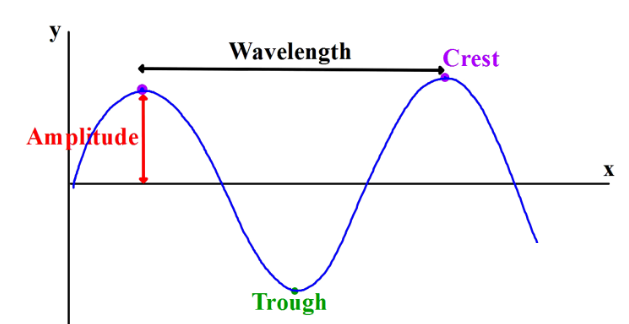
\includegraphics[width =\linewidth]{pic/transversale.png}
                        \end{minipage}
                        \begin{minipage}{0.49\linewidth}
                            longitudinal \\
                            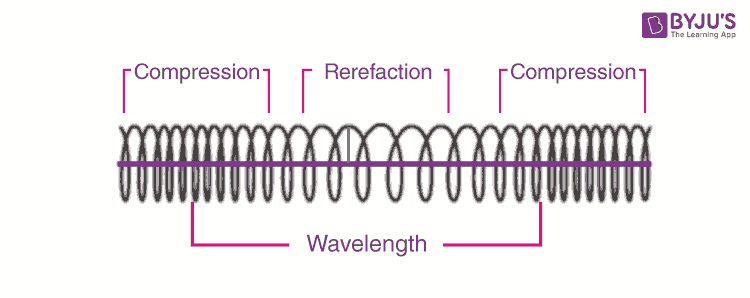
\includegraphics[width =\linewidth]{pic/longitudinal.png}
                        \end{minipage}
                    \item stationaires \\ 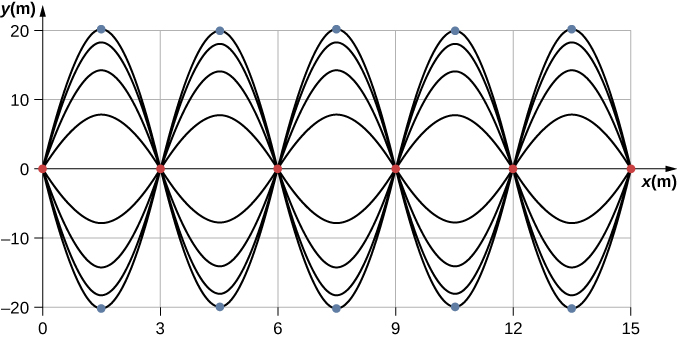
\includegraphics[width = 0.6\linewidth]{pic/stationair.jpg}
                \end{itemize}
        \section{Fonction d'onde}
            \begin{itemize}
                \item $f(x)$ : profil de londe (la form de la perturbation) 
                \item l onde qu' arrive au point(2) a temp $t$ est cell qui etait au point 1 a temp $ t- \frac{d}{c}$ tell que la distance entre 2 et 1 est $ d $
                \item $c$ est la celerite de l onde $ c= \frac{d}{\tau} $ avex $\tau $ est le temp necaissair pour la propagation entre 1 et 2 
                \item le term $ t - \frac{d}{c} $ est le temoindu caractere propagatif
                \item $\psi(x,t) $ : fonction d'onde tell que \\
                    $\psi(x,t) = f(t- \frac{x}{c}) $ (elle decri la propagation et le form)
                \item sense de propagation 
                    \begin{itemize}
                        \item si londe propage ver $x$ positive $\implies \psi(x,t) = f(x-\frac{x}{v})$
                        \item si londepropage ve x negative $\implies \psi(x,t) = f(t+ \frac{x}{v})$
                    \end{itemize}
                \item equation de propagation de l'onde \[\psi(x,t) = f(t-\frac{x}{v})=f[\frac{-1}{v}(x-vt)]=f(x-vt)\]
                \item On etude les ondes plan et harmonique car 
                    \begin{itemize}
                        \item tous ondes a trois dimension peut etre decompose on des ondes planes
                        \item tous onde periodique no harmonique peut etre decompose par la transformation de fourier sous form de superposition de plusieur ondes harmonique
                        \item tous ondes no periodique no harmonique on peut le transforme par integrale de fourier sous form des ondes harmonique
                    \end{itemize}
            \end{itemize}
        \section{Vitess de phase}
            c est la celerite de l onde monochromatique  (c est la vitesse d un point de phase donne)
            \[v_\varPhi = \frac{w}{k}\]
        \section{Vitess de group}
            C est la vitesse de propagation d un groupe d' onde 
        \section{Types des ondes}
            \begin{minipage}{0.49\linewidth}
                circulair \\
                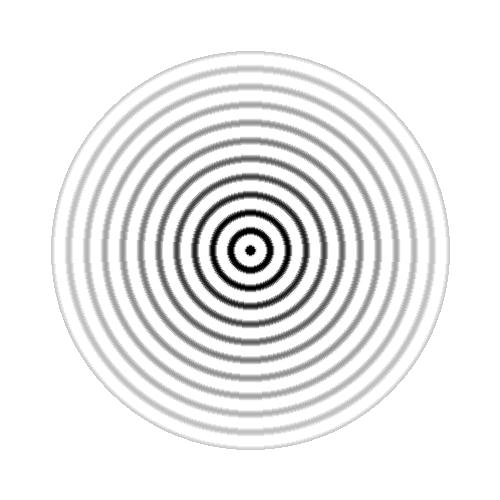
\includegraphics[width =\linewidth]{pic/circluair.jpg}
            \end{minipage}
            \begin{minipage}{0.49\linewidth}
                Planes \\
                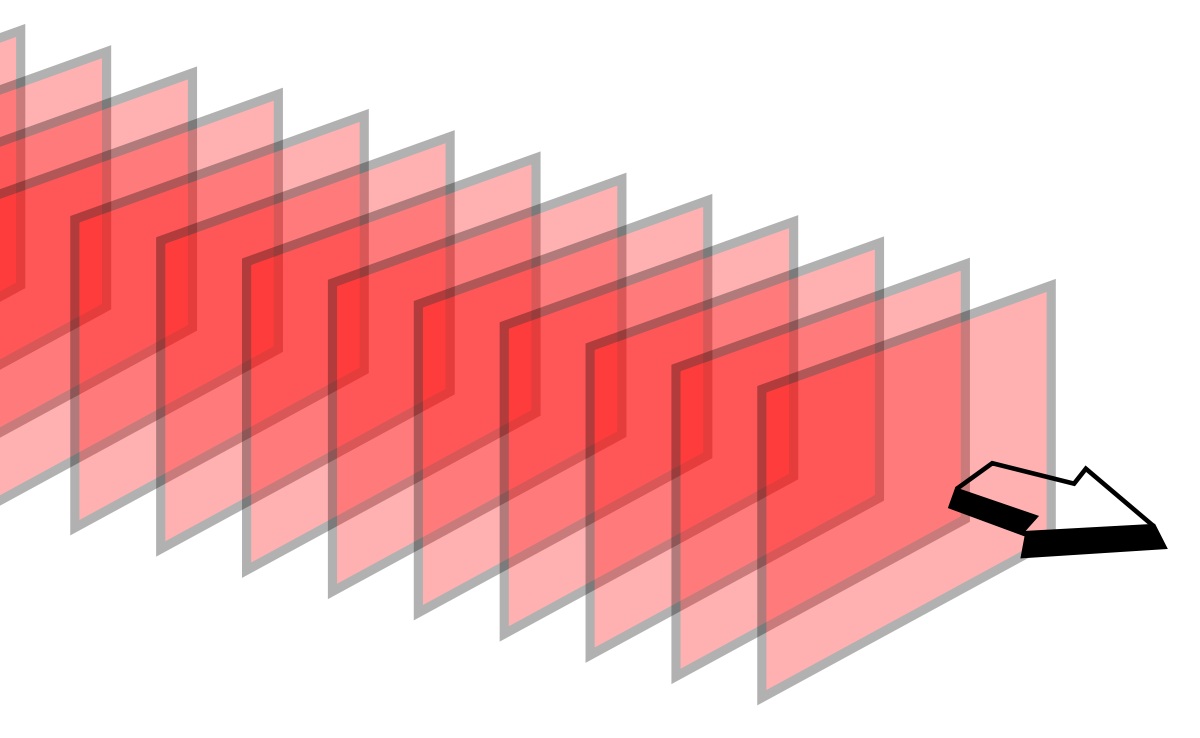
\includegraphics[width =\linewidth]{pic/Plane.png}
            \end{minipage}\\
            \begin{minipage}{0.49\linewidth}
                Cylindrique \\
                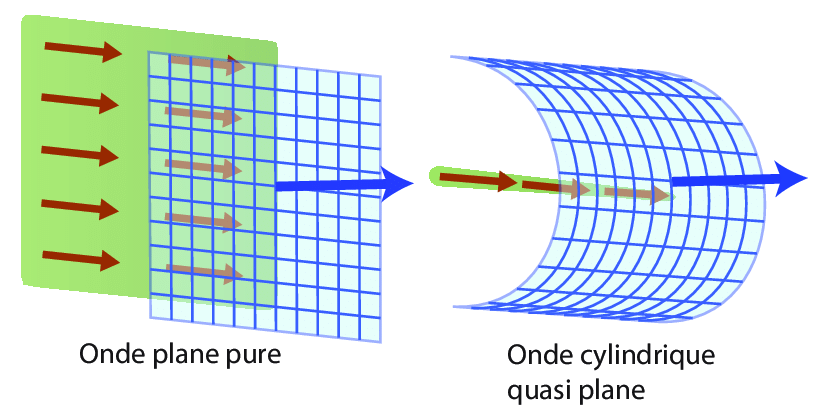
\includegraphics[width =\linewidth]{pic/cylindrique.png}
            \end{minipage}
            \begin{minipage}{0.49\linewidth}
                Spherique \\
                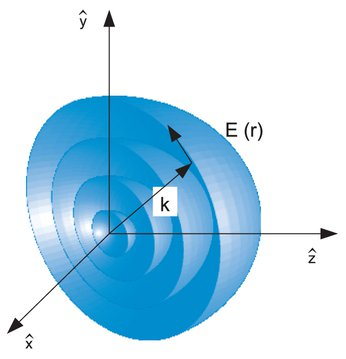
\includegraphics[width =\linewidth]{pic/spherique.jpg}
            \end{minipage}
            
            \underline{Note :} 
                \begin{itemize}
                    \item $\vec{k}$ toujour perpendiculaire au plan du fron onde ($\vec{k}$ est radial pour les ondes spherique et cylindrique $\implies \vec{k}.\vec{r}=kr$) 
                    \item les fonction des ondes sont les solution de l equation $\Delta \psi - \frac{\partial \psi^2}{v^2 \partial t^2} =0$ 
                \end{itemize}
            \underline{Front onde :} est l ensemble des point qui vibre en phase ( perpendiculair a la direction du propagation)

    \chapter{Theorie electromagnetique et propagation de la lumiere}
        \section{Equation de propagation de $\vec{E}$ et $\vec{B}$ }
            \subsection{Equation de maxwell}
                \begin{itemize}
                    \item $\vec{\Delta}.\vec{E} = \frac{\rho}{\varepsilon}$
                    \item $\vec{\nabla}.\vec{E} = \frac{-\partial \vec{B}}{\partial t}$
                    \item $\vec{\nabla}.\vec{B} = 0 $
                    \item $\vec{\nabla}\wedge\vec{B} = \mu \vec{J} + \mu \varepsilon \frac{\partial\vec{E}}{\partial t} $
                \end{itemize}
                \underline{Note :} dans l air ( milieux dielctrique) $\vec{J} =0 $ pas des charge libre $ \rho =0 $ 
                    \[ \vec{\Delta}.\vec{E} =0\]
                    \[ \vec{\nabla}\wedge\vec{B} =0\]
            \subsection{Equation de propagation de $\vec{E}$}
                \begin{itemize}
                    \item $\vec{\nabla}\wedge(\vec{\nabla}\wedge\vec{E}) =\vec{\nabla}.(\vec{\nabla.\vec{E}}) - \Delta\vec{E} = -\Delta\vec{E}$
                    \item $\vec{\nabla}\wedge(\vec{\nabla}\wedge\vec{E}) = \vec{\nabla}\wedge(\frac{-\partial\vec{B}}{\partial t})= - \frac{\partial}{-\partial t} \vec{\nabla}\wedge\vec{B} =\mu\varepsilon\frac{\partial^2\vec{E}}{\partial t^2}$
                    \item alors $-\Delta\vec{E} = -\mu\varepsilon\frac{\partial^2\vec{E}}{\partial t^2} \implies \Delta\vec{E} -\mu\varepsilon\frac{\partial^2\vec{E}}{\partial t^2} =\vec{0}$
                    \item \begin{center}
                        \boxed{  \Delta \vec{E} - \frac{1}{v^2}\frac{\partial^2\vec{E}}{\partial t^2} =0} 
                        avec $ v= \frac{1}{\sqrt{\mu\varepsilon}}$
                        \end{center}
                \end{itemize}
            \subsection{Equation de propagation de $\vec{B}$}
                \begin{itemize}
                    \item $\vec{\nabla}\wedge(\vec{\nabla}\wedge\vec{B}) =\vec{\nabla}.(\vec{\nabla.\vec{B}}) - \Delta\vec{B} = -\Delta\vec{B}$
                    \item $\vec{\nabla}\wedge(\vec{\nabla}\wedge\vec{B}) = \vec{\nabla}\wedge(\mu\varepsilon\frac{\partial\vec{E}}{\partial t} )= \mu \varepsilon \frac{\partial}{\partial t}(-\frac{\partial \vec{B}}{\partial t}) = -\mu\varepsilon\frac{\partial^2\vec{B}}{\partial t^2}$
                    \item alors $\Delta \vec{B} - \mu \varepsilon \frac{\partial^2\vec{B}}{\partial t^2} = \vec{0}$
                    \item \begin{center}
                        \boxed{ \Delta\vec{B} -\frac{1}{v^2}\frac{\partial^2\vec{B}}{\partial t^2} = \vec{0}  } avec $ v= \frac{1}{\sqrt{\mu\varepsilon}}$
                    \end{center}


                \end{itemize}
        \section{Caractere transversal de l onde electromagnetique}
            Une onde electromagnetique est dite transversal si $\vec{E}$ et $\vec{B}$ sont $\perp $ a $\vec{k}$ .
            \\ soit une onde electromagnetique plane se propagent selon les x positive dans ce plan la phase $\vec{E}$ et $\vec{B}$ no varie pas $\forall$ y et z 
            \begin{itemize}
                \item $\vec{E}$ et $\vec{B}$ sont independant de y et z
                \item $\vec{E}$ et $\vec{B}$ dependent seulment de x et de t
            \end{itemize}
            ona $ \vec{\nabla}.\vec{E} =0 \implies \frac{\partial E_x}{\partial x} + \frac{\partial E_y}{\partial y} + \frac{\partial E_z}{\partial z} =0 $ \\
            $ \frac{\partial E_y}{\partial y} =0 $ et $  \frac{\partial E_z}{\partial z} =0 $ donc $ \frac{\partial E_x}{\partial x} =0 \implies E_x =0  , E_x \not = 0$ est impossible (propagation) \\
            $\vec{E} $ n a pas de composant selon x $ \implies \vec{E} \perp \vec(x)$ \\
            meme calcule pour $\vec{B} $ on utilize $\vec{\nabla}\vec{B}=0 \ldots $ \\
            \underline{Alors :}
                \begin{itemize}
                    \item $\vec{E}$ perpendiculair a la direction de propagation
                    \item $\vec{B}$ perpendiculair a la direction de propagation
                    \item $\vec{E}$ et $\vec{B}$ dependent de x
                    \item $\vec{E} \perp \vec{B}$ ( $\vec{\nabla}\wedge\vec{E} = -\frac{\partial \vec{B}}{\partial t}$) 
                    \item \boxed{E = Bv} ou $v = \frac{1}{\sqrt{\mu\varepsilon}}$ $v$ est la vitess de propagation
                    \item $\vec{E}$ et $\vec{B}$ son en phase \\ 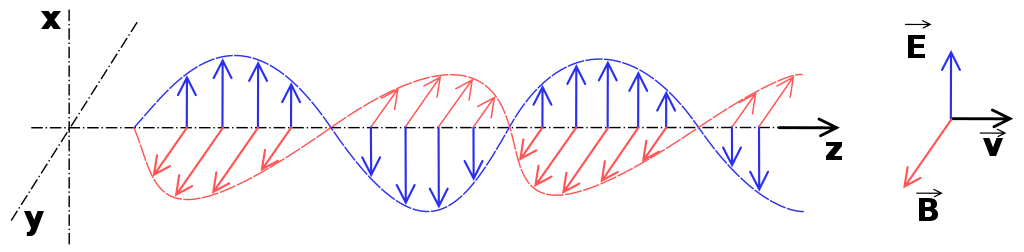
\includegraphics[width = 0.6\linewidth]{pic/Onde_electromagnetique.png}
                \end{itemize}
        \section{Energie transporte par l onde electromagnetique}
            \begin{itemize}
                \item Toute onde se propage transport avec ell de l' Energiele 
                \item Puissance electromagnetique est le quantite de l energie par unite de temps qui travers une section $s$
                    \[ P = \frac{dw}{dt} = \iint \vec{S}.d\vec{s}\] avec $\vec{S}$ est la densite de puissance ( vecteur de poynting)
                \item Vecteur de poynting $\vec{S}$ \[ \vec{S} = \frac{1}{\mu}\vec{E}\wedge\vec{B} = \vec{E}\wedge\vec{H} \]
                \item Puissance moyene \[ \langle P \rangle  =\iint \langle \vec{S}\rangle .d\vec{s}\]
                \item densite moyene de puissance \[ \langle \vec{S} \rangle  = \langle \frac{1}{\mu}\vec{E}\wedge\vec{B} \rangle = \langle \vec{E}\wedge\vec{H} \rangle \]
                \item eclairement $I$ \[ I = | \langle \vec{S} \rangle| \]
                \item Debit $D$ \[ D = |\vec{S}| = |\frac{1}{\mu}\vec{E}\wedge\vec{B}| =\frac{EB}{\mu} = \varepsilon E v\] 
                    \[D =uv\] ($u$ : densite d denergie electromagnetique)
                \item Densite d' energie electromagnetique \\
                    la densite d energie electromagnetique est lasomme de densite d'energie magnetique $(u_B)$ et celle d'electrique $(u_E)$
                    \[ u_e = \frac{1}{2}\vec{D}.\vec{E}=\frac{1}{2}\varepsilon E^2  \]
                    \[ u_b = \frac{1}{2}\vec{B}.\vec{H}=\frac{1}{2}\frac{E^2}{\mu v^2} = \frac{1}{2}\varepsilon E^2 \]
                    alors $(u_B = u_E)$ \\
                    $u = 2u_E=2u_B=\frac{1}{\mu}B^2 = \varepsilon E^2$

            \end{itemize}
        \section{Relation entre les champ electrique (incident , reflechi et transmie)}
            \underline{Propriete mathematique :} 
            \begin{itemize}
                \item Si $\vec{k}$ est perpendiculaire au plan contenant $M(x,y,z) \implies \vec{k}.\vec{r} = cte$ avec $\vec{r}=\vv{OM}$
                \item Si $vv{k}.\vv{r} =cte \implies \vv{k} $ perpendiculair au plan contenant $M$ 
                \begin{center}
                    \boxed{\vv{k}.\vv{r} = cte \Leftrightarrow \vv{k}\wedge\vv{n}=\vv{0} } \\
                    avec $\vv{n}$ perpendiculair au plan
                \end{center}
            \end{itemize}
            \underline{La relation :} 
            \begin{center}
                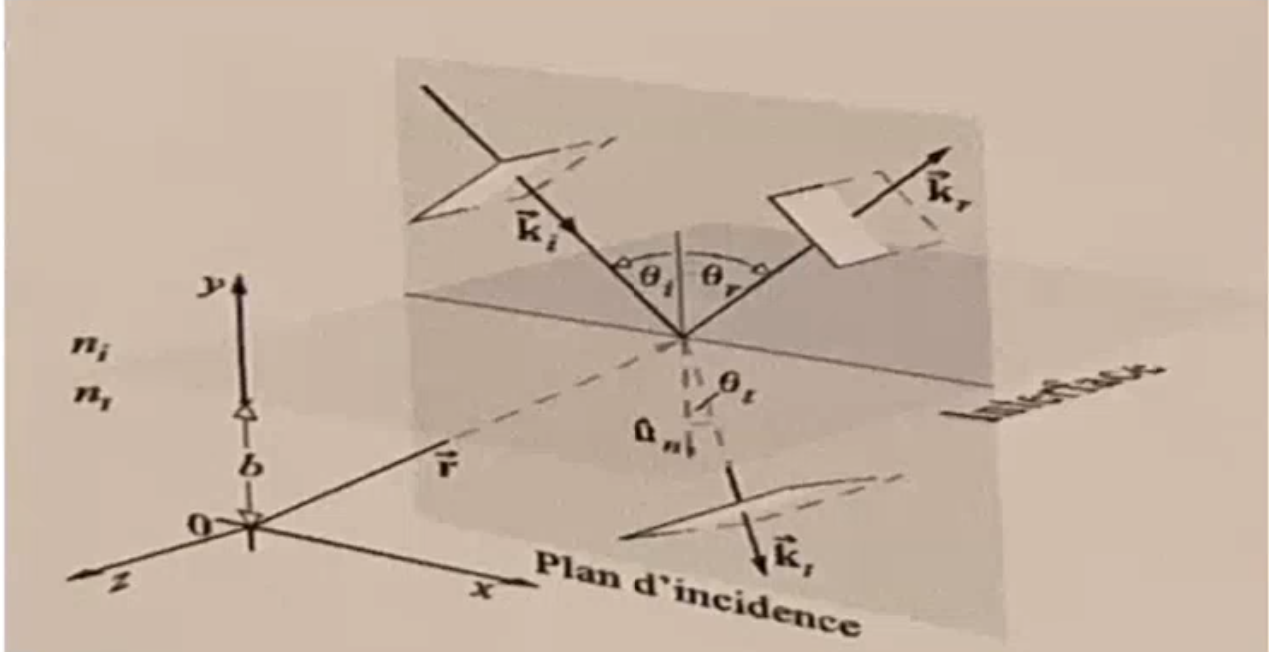
\includegraphics[width = 0.6\linewidth]{pic/incident_reflechie_transmims.png}
            \end{center}
            \underline{on a :} \\
                $ \vv{E_i} = \vv{E_{0i}}\cos(\vv{k_i}.\vv{r}-w_it) $ \\
                $ \vv{E_r} = \vv{E_{0r}}\cos(\vv{k_i}.\vv{r}-w_it + \varphi_{0r}) $ \\
                $ \vv{E_t} = \vv{E_{0t}}\cos(\vv{k_i}.\vv{r}-w_it + \varphi_{0t}) $ \\
                
                \begin{center}
                    dapres la continuite de composant tangentielle du champ electrique on a \\
                    $ \vv{n_{12}}\wedge(\vv{E_1}) = \vv{n_{12}}\wedge(\vv{E_2}) $ avec \\ $\vv{E_1} $ est le vecteur champ electrique dans le milieu 1 \\ et $\vv{E_2} $ est le vecteur champ electrique dans le milieu 2
                \end{center}
                    $ \vv{n_{12}}\wedge(\vv{E_{0i}}\cos(\vv{k_i}.\vv{r}-w_it) +  \vv{E_{0r}}\cos(\vv{k_i}.\vv{r}-w_it + \varphi_{0r})) = \vv{n_{12}}\wedge( \vv{E_{0t}}\cos(\vv{k_i}.\vv{r}-w_it + \varphi_{0t})) $
                    \\ $\implies \vv{k_i}\vv{r}-w_it =\vv{k_r}-w_rt + \varphi_{0r} = \vv{k_t} -w_t + \varphi_{ot}$
                    \begin{center}
                        Alors  \boxed{w_i = w_r = w_t} \\ 
                        (la lumiere incident , transmis et reflechie a la meme frequence)
                    \end{center}
                $\vv{k_i}.\vv{r}=\vv{k_r}\vv{r}+ \varphi_{0r}$ \\
                $\implies(\vv{k_i}-\vv{k_r})\vv{r} = \varphi_{0r}= cte \implies \vv{n_{12}} \wedge(\vv{k_i}-\vv{k_r}) = \vv{0}$ \\
                $\implies \vv{n_{12}} \wedge(\vv{k_i}) = \vv{n_{12}}\wedge(\vv{k_r})$ \\
                $\implies k_i\sin(\theta_i) = k_r\sin(\theta_r)$ \\
                \begin{center}
                    mais $k_i$ et $k_r$ sont egaux (meme milieu) \\
                    \boxed{\theta_i = \theta_r}
                \end{center}
                $ \vv{k_i}\vv{r} = k_t\vv{r} + \varphi_{0t} $\\ 
                $\implies(\vv{k_i}-\vv{k_t}).\vv{r} = \varphi_{0t} = cte \implies \vv{n_{12}} (\vv{k_i}-\vv{k_t}) = \vv{0}$
                $\implies \vv{n_{12}} \wedge(\vv{k_i}) = \vv{n_{12}}\wedge(\vv{k_t})$ \\
                \begin{center}
                    \boxed{k_i\sin(\theta_i) = k_r\sin(\theta_t)} \\
                    avec $k_i = \frac{w_i}{v_i} =\frac{w_i}{\frac{c}{n_i}}=n_i\frac{w}{c} $ et $k_t=n_t \frac{w}{c}$
                \end{center} 
        \section{Polarisation perpendiculaire et parallele}
                \begin{center}
                    \begin{minipage}{0.49\linewidth}
                        \underline{Polarisation parallel} \\
                        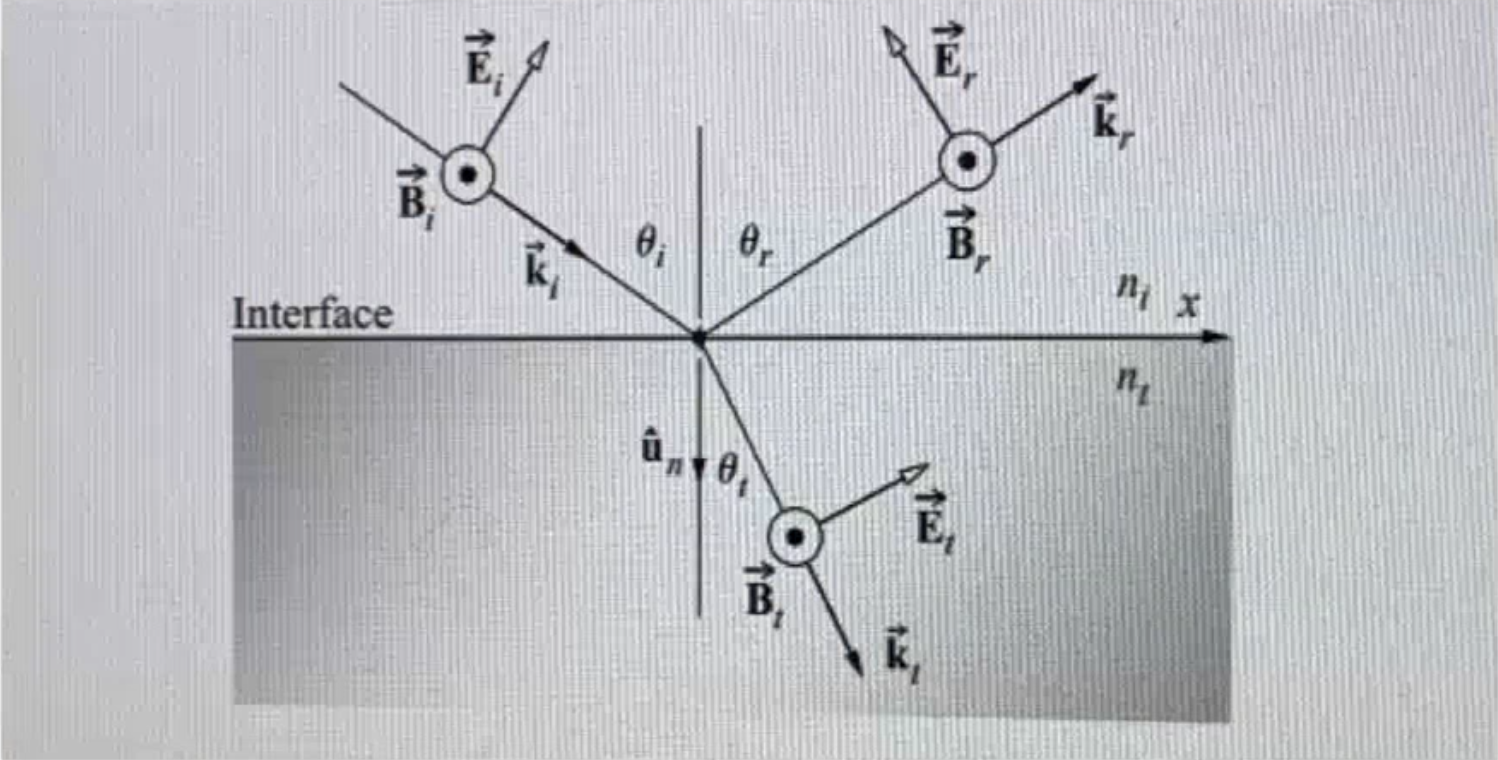
\includegraphics[width =\linewidth]{pic/polarisationpar.png}
                    \end{minipage}
                    \begin{minipage}{0.49\linewidth}
                        \underline{Polarisation perpendiculair} \\
                        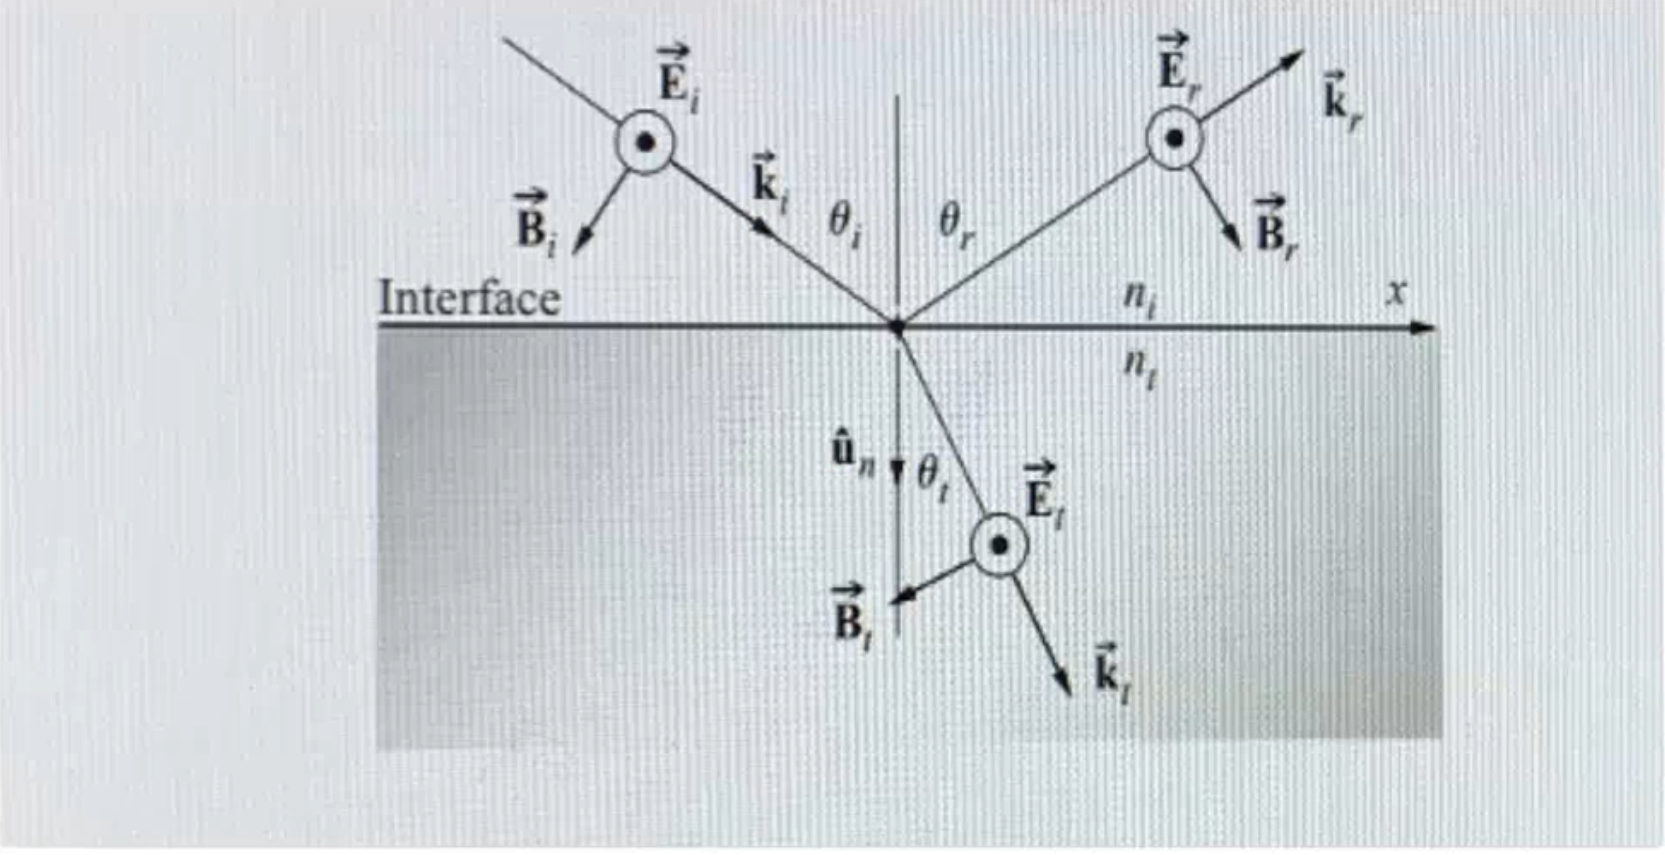
\includegraphics[width = \linewidth]{pic/polarisationperp.png}
                    \end{minipage}
                \end{center}
        \section{coefficient de reflexion et de transmission }
            \subsection{polarisation perpendiculair}
                $\vv{u}$
                \begin{itemize}
                    \item $\vv{u_i} = -\cos(\theta_i\vv){u_y} + \sin(\theta_i)\vv{u_x}$
                    \item $\vv{u_r} = \cos(\theta_r\vv){u_y} + \sin(\theta_r)\vv{u_x}$
                    \item $\vv{u_i} = -\cos(\theta_t\vv){u_y} + \sin(\theta_t)\vv{u_x}$
                \end{itemize}
                $\vv{k}$
                \begin{itemize}
                    \item $\vv{k_i} = k_i\vv{u_i}$
                    \item $\vv{k_r} = k_r\vv{u_r}$
                    \item $\vv{k_t} = k_t\vv{u_t}$
                \end{itemize}
                $\vv{k_r}$
                \begin{itemize}
                    \item $\vv{k_i}\vv{r} = k(-\cos(\theta_i)y+\sin(\theta_i)x)$
                    \item $\vv{k_r}\vv{r} = k(-\cos(\theta_r)y+\sin(\theta_i)x)$
                    \item $\vv{k_t}\vv{r} = k(-\cos(\theta_t)y+\sin(\theta_i)x)$
                \end{itemize}
                Champ electrique
                \begin{itemize}
                    \item $ \vv{E_i} = \vv{u_z}A_ie^{i(wt-\vv{k_i}\vv{r})} =\vv{u_z}A_ie^{i(wt-k_i(-\cos(\theta_i)y +\sin(\theta_i)x))}$
                    \item $ \vv{E_r} = \vv{u_z}A_re^{r(wt-\vv{k_i}\vv{r})} =\vv{u_z}A_re^{r(wt-k_i(\cos(\theta_r)y +\sin(\theta_r)x))}$
                    \item $ \vv{E_r} = \vv{u_z}A_te^{r(wt-\vv{k_t}\vv{r})} =\vv{u_z}A_te^{r(wt-k_t(-\cos(\theta_t)y +\sin(\theta_t)x))}$
                \end{itemize}
                Champ magnetique
                \begin{itemize}
                    \item $\vv{B_i} = \frac{\vv{u_i}}{v_i}\wedge\vv{E_i} =\frac{1}{v_i}(-\cos(\theta_i)\vv{u_x}-\sin(\theta_i)\vv{u_y})A_ie^{i(wt-k_i(-\cos(\theta_i)y +\sin(\theta_i)x))}$
                    \item $\vv{B_r} = \frac{\vv{u_r}}{v_r}\wedge\vv{E_r} =\frac{1}{v_r}(\cos(\theta_r)\vv{u_x}-\sin(\theta_r)\vv{u_y})A_re^{r(wt-k_i(\cos(\theta_r)y +\sin(\theta_r)x))}$
                    \item $\vv{B_t} = \frac{\vv{u_i}}{v_t}\wedge\vv{E_t} =\frac{1}{v_t}(-\cos(\theta_t)\vv{u_x}-\sin(\theta_t)\vv{u_y})A_te^{r(wt-k_t(-\cos(\theta_t)y +\sin(\theta_t)x))}$
                \end{itemize}
                \begin{center}
                    $k_i =k_r =k_1 , k_t =k_2$ \\
                    $A_i = E_{0i}e^{i\vartheta_{0i}} , A_r = E_{0r}e^{i\vartheta_{0r}} , A_t = E_{0t}e^{i\vartheta_{0t}}$
                \end{center}
                \pagebreak
                Soit :
                \begin{itemize}
                    \item $\vv{E_1}$ le champ electrique resultant dans le milieu (1)
                    \item $\vv{E_2}$ le champ electrique resultant dans le milieu (2)
                    \item $\vv{B_1}$ le champ magnetique resultant dans le milieu (1)
                    \item $\vv{B_2}$ le champ magnetique resultant dans le milieu (2)
                \end{itemize}
                \begin{center}
                    \boxed{\vv{E_1} = \vv{E_r} +\vv{E_i} , \vv{E_2} = \vv{E_t}} \\
                    \boxed{\vv{B_1} = \vv{B_r} +\vv{B_i} , \vv{B_2} = \vv{B_t}}
                \end{center}
                \underline{Continuuite de compossant tangentielle de champ electrique $\vv{E} (\vv{E_{1tg}}=\vv{E_{2tg}})$}
                    \\ pour $y=0 , \vv{E_{1tg}}=\vv{E_{2tg}} $
                    \[\vv{u_z}A_ie^{i(wt-k_i(\sin(\theta_i)x))} + \vv{u_z}A_re^{r(wt-k_i(+\sin(\theta_r)x))}  =\vv{u_z}A_te^{r(wt-k_t(+\sin(\theta_t)x))} \]
                    puisque \boxed{k_i\sin(\theta_i) = k_r\sin(\theta_t)} et \boxed{\theta_i = \theta_r} Alors
                \begin{center}
                    \boxed{A_i + A_r =A_t} (equation 1)
                \end{center}
                \underline{continuite de composant tangentielle de $\vv{H}$} \\
                    $\vv{n_{12}}\wedge(H_2 - H_1) = \vv{J} = \vv{0}$ (milieu no condicteur) \\
                    $\vv{H_{1tg}}=\vv{H_{2tg}}$ avec $B= \mu H$ \\
                    $\vv{B_i} = \mu_1 \vv{H_i} , \vv{B_r} = \mu_1 \vv{H_r} , \vv{B_t} = \mu_2 \vv{H_t}$
                    mais $\mu_1 =\mu_2$ ( milieu conc magnetique)\\
                    alors $\vv{B_{1tg}}=\vv{B_{2tg}}$\\
                    \[ \frac{1}{v_i}(-\cos(\theta_i)\vv{u_x})A_ie^{i(wt-k_i(\sin(\theta_i)x))} +  \frac{1}{v_r}(\cos(\theta_r)\vv{u_x})A_re^{r(wt-k_i(\sin(\theta_r)x))}  =  \frac{1}{v_t}(-\cos(\theta_t)\vv{u_x}A_te^{r(wt-k_t(\sin(\theta_t)x))}\]
                    puisque \boxed{k_i\sin(\theta_i) = k_r\sin(\theta_t)} et \boxed{\theta_i = \theta_r} Alors \\
                \begin{center}
                    \boxed{\frac{1}{v_i}(-\cos(\theta_i)A_i )+ \frac{1}{v_r}\cos(\theta_r)A_r=  \frac{1}{v_t}(-\cos(\theta_t))A_t } (equation 2)
                \end{center}
                \underline{La solution de system d'equation (1) et (2)} 
                    \[ A_r = \frac{n_i\cos(\theta_i) -n_t\cos(\theta_t)}{n_i\cos(\theta_i) +n_t\cos(\theta_t)}A_i \]
                    \[ A_t = \frac{2n_i\cos(\theta_i)}{n_i\cos(\theta_i) +n_t\cos(\theta_t)}A_i \]
                \begin{center}
                    avec $v_1 = \frac{c}{n_i}$ et $v_2 = \frac{c}{n_t}$
                \end{center}
                \underline{Coefficient de reflexin $r_\perp$}
                \begin{center}
                    \boxed{r_\perp = \frac{A_{r_\perp} }{A_{i_\perp}} = \frac{n_i\cos(\theta_i) -n_t\cos(\theta_t)}{n_i\cos(\theta_i) +n_t\cos(\theta_t)}}
                \end{center}
                \underline{Coefficient de transmision $t_\perp$}
                \begin{center}
                    \boxed{t_\perp = \frac{A_{t_\perp} }{A_{i_\perp}} = \frac{2n_i\cos(\theta_i)}{n_i\cos(\theta_i) +n_t\cos(\theta_t)}}
                \end{center}
            \subsection{polarisation parallel}
                la method est tres proche de celle dans la polarisation perpendiculair \\
                \underline{Coefficient de reflexin $r_\parallel$}
                \begin{center}
                    \boxed{r_\parallel = \frac{A_{r_\parallel} }{A_{i_\parallel}} = \frac{n_t\cos(\theta_i) -n_i\cos(\theta_t)}{n_t\cos(\theta_i) +n_i\cos(\theta_t)}}
                \end{center}
                \underline{Coefficient de transmision $t_\parallel$}
                \begin{center}
                    \boxed{t_\parallel = \frac{A_{t_\parallel} }{A_{i_\parallel}} = \frac{2n_i\cos(\theta_i)}{n_t\cos(\theta_i) +n_i\cos(\theta_t)}}
                \end{center}
                \underline{Note :} \\
                \begin{center}
                    \boxed{1+r_\perp = t_\perp }
                    \boxed{(1-r_\parallel) = \frac{\cos(\theta_t)}{\cos(\theta_i)}t_\parallel}
                \end{center}
                \pagebreak
        \section{Angle critique de reflexion total}
            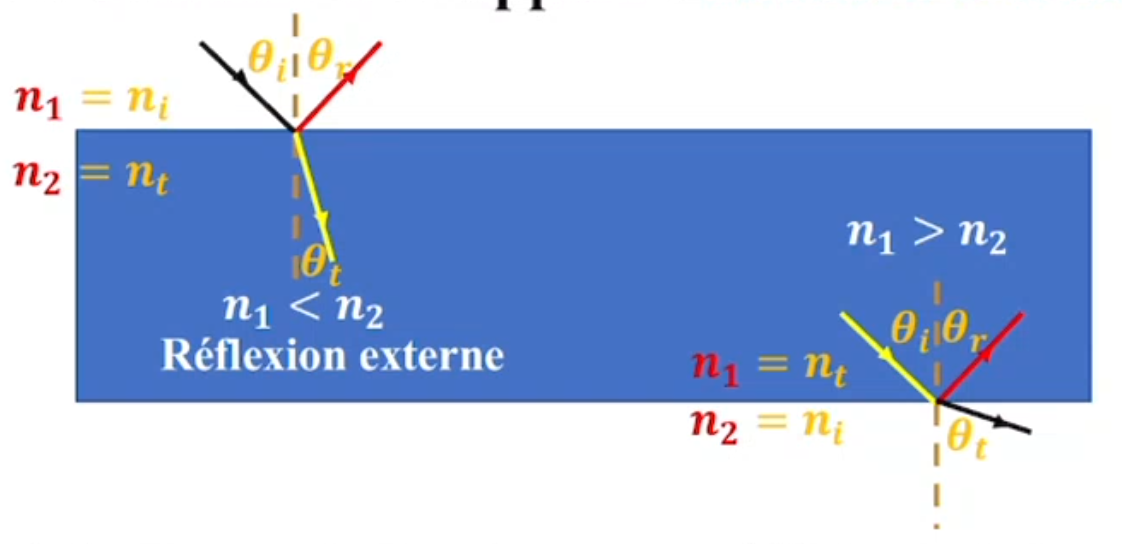
\includegraphics[]{pic/anglecritique.png}
            \begin{itemize}
                \item Si $n_1 < n_2$ , $\theta_t < \theta_i \implies $ reflexion partielle ( reflexion externe)
                \item Si $n_1 > n_2$ , $\theta_t > \theta_i \implies $ reflexion interne et possibilite d une reflexion total si $\theta_i > \theta_c$
            \end{itemize}
            \underline{avex $\theta_c$ est l angle critique}
        \section{Angle critique du reflexion totale en polarisation parallele et perpendiculair}
            \subsection{Chercher $\cos(\theta_t)$ dans une reflexion complete}
                \underline{on a :} \\
                $n_1\sin(\theta_i) = n_2\sin(\theta_t)$ \\
                pour obtien l angle critique $\theta_c $ , $\theta_t $ doit etre egal a $\frac{\pi}{2}$ \\
                alors $\sin(\theta_c) = \frac{n_t}{n_i} =n_{ti}$\\
                \underline{dans le cas ou $\theta_i > \theta_c$ ona :}\\
                $ \sin(\theta_i) > \sin(\theta_c) \implies \sin(\theta_i) > n_{ti} \implies \sin(\theta_i)^2 > n_{ti}^2 \implies n_{ti}^2 - \sin(\theta_i)^2 < 0 $\\
                $n_{ti}^2 - \sin(\theta_i)^2 = -(\sin(\theta_i)^2-n_{ti}^2) = i^2(\sin(\theta_i)^2 -n_{ti})^2$ \\
                Alors  \\
                \begin{center}
                    \boxed{\sqrt{n_{ti}^2 -\sin(\theta_i)^2 } = \pm i\sqrt{\sin(\theta_i)^2 -n_{ti}^2} } \\
                    equation (1)
                \end{center}
                \begin{itemize}
                    \item ona : $ \cos(\theta_t) = \sqrt{1-\sin(\theta_t)} $ et $ n_i\sin(\theta_i) = n_t\sin(\theta_t) \implies \sin(\theta_t) = \frac{\sin(\theta_i)}{n_{ti}} $
                    \item remplacon $\sin(\theta_t)$ par sa valeur $\cos(\theta_t) = \sqrt{1-\frac{\sin(\theta_i)}{n_{ti}}} = \frac{1}{n_{ti}}\sqrt{n_{ti}^2 - \sin(\theta_i)^2} $
                    \item utilisent l equation (1) : \\
                        \begin{center}
                            $\cos(\theta_t) = \pm \frac{i}{n_{ti}}\sqrt{\sin(\theta_i)^2 - n_{ti}^2} $ (2)\\
                            mais la solution acceptable physiquement est le (-)
                        \end{center}
                    \item \underline{Preuve de la sign (-) de l equation (2)} \\
                        prenons $\vv{E_t}$ en polarisation perpendiculair $\vv{E_t} = \vv{u_z}A_te^{i(wt-\vv{k_t}\vv{r})}$\\
                        $\vv{E_t} = \vv{u_z}A_te^{iwt}e^{ik_2\cos(\theta_t)y}e^{-ik_2\sin(\theta_t)x}$ \\
                        avec $y < 0$ et $\cos(\theta_t) = - \frac{i}{n_{ti}}\sqrt{\sin(\theta_i)^2 - n_{ti}^2} < 0$
                        \begin{center}
                            alors $e^{ik_2\cos(\theta_t)y}\to 0$ , car $ik_2\cos(\theta_t)y \to -\infty$ en progresson avec y \\
                            qui est \underline{Physiquement vrai} ($E_t \to 0$ dans une reflexion complete)
                        \end{center}
                        mais si on prendre $+ \frac{i}{n_{ti}}\sqrt{\sin(\theta_i)^2 - n_{ti}^2} \implies$ $e^{ik_2\cos(\theta_t)y}\to +\infty$ , car $ik_2\cos(\theta_t)y \to +\infty$ en progresson avec y \\
                        qui est \underline{Physiquement impossible} ($E_t \to 0$ dans une reflexion complete)
                    \item \underline{Note :} dans une reflexion totale $\vv{E_t} \not = 0$ mais il derige vers $0$ exponentiellment
                    \item \begin{center}
                        \boxed{\cos(\theta_t) = - \frac{i}{n_{ti}}\sqrt{\sin(\theta_i)^2 - n_{ti}^2} }
                    \end{center}
                \end{itemize}
            \subsection{Coefficient de reflexoin}
                On a exprime $\cos(\theta_t)$ en form complex et en fonction de $\theta_i$ . \\
                maintenant en peut exprimer $r_\perp^\parallel$ sans $\theta_t$ en remplacent $\cos(\theta_t)$ par ca valeur \\
                \[ r_\parallel = \frac{E_{0r_\parallel}}{E_{0i_\parallel}} e^{i\Delta\Phi_\parallel} = - \frac{ n_{ti}^2\cos(\theta_i)+i\sqrt{\sin(\theta_i)^2 - n_{ti}^2 }}{-n_{ti}^2\cos(\theta_i)+\sqrt{\sin(\theta_i)^2 - n_{ti}^2 }} = e^{i\pi}\frac{\rho_{r_\parallel} e^{i\Phi_{r_\parallel}} }{\rho_{i_\parallel} e^{i\Phi_{i_\parallel}}}  \]
                \begin{center}
                    \boxed{r_\parallel = e^{i\pi}e^{i\Delta\Phi_\parallel}}
                \end{center}
                \[ r_\perp = \frac{E_{0r_\perp}}{E_{0i_\perp}} e^{i\Delta\Phi_\perp} = - \frac{ \cos(\theta_i)+i\sqrt{\sin(\theta_i)^2 - n_{ti}^2 }}{\cos(\theta_i)+i\sqrt{\sin(\theta_i)^2 - n_{ti}^2 }} = e^{i\pi}\frac{\rho_{r_\perp} e^{i\Phi_{r_\perp}} }{\rho_{i_\perp} e^{i\Phi_{i_\perp}}}  \]
                \begin{center}
                    \boxed{r_\perp = e^{i\pi}e^{i\Delta\Phi_\perp}}
                \end{center}
                \underline{Note :} ($\rho$) la module de coefficient de reflexion est egal a 1 , en peut verifier ca utilisent
                    \begin{center}
                        $| r |^2 = r.r^*$
                    \end{center}
            \subsection{$\Delta\Phi_\perp$ et $\Delta\Phi_\parallel$}
                    Puisque $r_\perp$ et $r_\parallel$ sont des nombres complex alors en peut chercher $\Delta\Phi_\perp$ et $\Delta\Phi_\parallel$ en cherchent l argument des $r_\perp$ et $r_\parallel$ 
                    \begin{center}
                        \boxed{\Delta\Phi_\parallel = \pi + 2\arctan(\frac{ \sqrt{\sin(\theta_i)^2 - n_{ti}^2} }{ n_{ti}^2\cos(\theta_i) } ) }
                        \boxed{\Delta\Phi_\perp = \pi + 2\arctan(\frac{ \sqrt{\sin(\theta_i)^2 - n_{ti}^2} }{\cos(\theta_i) } ) }
                    \end{center}
        \section{Coefficient de reflexion et transmission en fonction des impedance intrinseques $\eta$}
            \[\eta = \frac{\mu c}{n}\]
            \[ r_\parallel = \frac{\eta_i \cos(\theta_i)-\eta_t\cos(\theta_t)}{\eta_i \cos(\theta_i)+\eta_t\cos(\theta_t)}\]
            \[ t_\parallel = \frac{2\eta_i \cos(\theta_i)}{\eta_i \cos(\theta_i)+\eta_t\cos(\theta_t)}\]
            \[ r_\perp = \frac{\eta_t \cos(\theta_i)-\eta_i\cos(\theta_t)}{\eta_t \cos(\theta_i)+\eta_i\cos(\theta_t)}\]
            \[ t_\perp = \frac{2\eta_t \cos(\theta_i)}{\eta_t \cos(\theta_i)+\eta_i\cos(\theta_t)}\]
        \section{Angle de Brewster }
            \begin{center}
                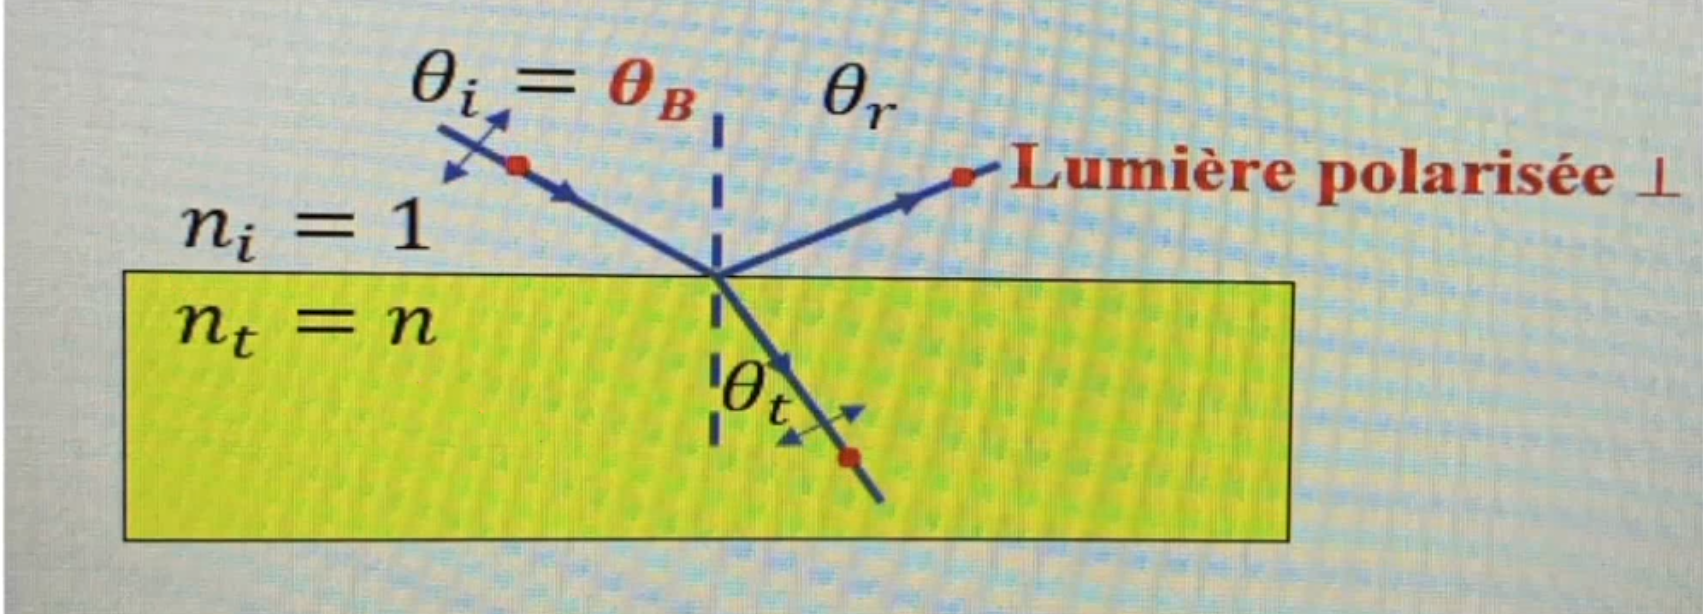
\includegraphics[width = 0.6\linewidth]{pic/brewster.png}
            \end{center}
            On appelle angle de Brewster $\theta_B$ l angle d incidence pour lequel il y a transmission total \\
            pour obtenir $\theta_B$ il faut anuler alors les coefficients de reflexion \\
            \begin{center}
                \boxed{r_\parallel = 0 \implies \eta_i\cos(\theta_i) = \eta_t\cos(\theta_t)}
                \boxed{r_\perp = 0 \implies \eta_t\cos(\theta_i) = \eta_i\cos(\theta_t)}
            \end{center}
            \begin{center}
                \underline{Note:} en peut obtenir $\theta_B$ par anuler les coefficients des reflexions car ces coefficient peut etre annuler , tandis que les coefficient de transmission en peut pas les anuler (equations des coefficient des transmision)
            \end{center}
            \subsection{$\theta_B$ pour les milieux magnetique (polarisation parallele) }
                $r_\parallel =0 \implies \eta_i\cos(\theta_i)=\eta_t\cos(\theta_t)$ \\
                $\implies \eta_i\sqrt{1-\sin(\theta_i)^2} = \eta_t\sqrt{1-\sin(\theta_t)^2}$ \\
                $\implies 1-\sin(\theta_i)^2 = (\frac{\eta_t}{\eta_i})^2(1-\sin(\theta_t)^2)$ \\
                on a $\eta = \mu\frac{c}{n}$ et $n_i \sin(\theta_i) = n_t\sin(\theta_t) \implies \sin(\theta_t) =\frac{\eta_t\mu_i}{\eta_i\mu_i}\sin(\theta_i)$\\
                remplacon la valeur de $\sin(\theta_t)$ : \\
                \[ (1-\sin(\theta_i))^2 = (\frac{\eta_t}{\eta_i})^2 \left[ 1-(\frac{\eta_t\mu_i}{\eta_t\mu_t}\sin(\theta_i))^2 \right] \]
                \[ (1-\sin(\theta_i))^2 = (\frac{\eta_t}{\eta_i})^2 - (\frac{\eta_t}{\eta_i})^4(\frac{\mu_i}{\mu_t})^2\sin(\theta_i)^2 \]
                \[ \sin(\theta_i)^2 = \frac{ 1- (\frac{\eta_t}{\eta_i})^2 }{ 1- (\frac{\eta_t}{\eta_i})^4(\frac{\mu_i}{\mu_t})^2 } \]
                Sachant que $\eta = \sqrt{\frac{\mu}{\varepsilon}} \implies \frac{\eta_t}{\eta_i}=\sqrt{\frac{\varepsilon_i\mu_t}{\varepsilon_t\mu_i}} $ \\
                \begin{center}
                    \boxed{\sin(\theta_i) = \sin(\theta_B) = \sqrt{\frac{ 1-\frac{\varepsilon_i\mu_t}{\varepsilon_t\mu_i} }{ 1-(\frac{\varepsilon_i}{\varepsilon_t})^2 }}}
                \end{center}
            \subsection{$\theta_B$ pour les milieux non magnetique $\mu_i = \mu_t$ (polarisation parallele) }
                \begin{center}
                    \boxed{\sin(\theta_B) = \sqrt{\frac{1}{1+\frac{\varepsilon_i}{\varepsilon_t}}} }
                \end{center}
            \underline{Note}\\
            en peut prouver que $r_\parallel = \frac{\tan(\theta_i - \theta_t)}{\tan(\theta_i + \theta_t)}$\\
            alors pour $r_\parallel =0 \implies \tan(\theta_i + \theta_t) = \infty \implies$ \boxed{\theta_i+\theta_t =\frac{\pi}{2}}
            \subsection{$\theta_B$ pour le milieu magnetique (polarisation perpendiculair)}
            meme methode que celle de polarisation parallel
            \begin{center}
                \boxed{\sin(\theta_i) = \sin(\theta_B) = \sqrt{\frac{ 1-\frac{\varepsilon_i\mu_t}{\varepsilon_t\mu_i} }{ 1-(\frac{\mu_i}{\mu_t})^2 }}}
            \end{center}
            \subsection{$\theta_B$ pour le milieu non magnetique $\mu_i = \mu_t$ (polarisation perpendiculair)}
            $\mu_i = \mu_t \implies \sin(\theta_B) = \infty$ qui est impossible \\
            alors $\theta_B$ pour les milieux non magnetique \underline{n exsite pas}
        \section{A quoi sert l'angle de Brewster}
        \begin{itemize}
            \item Cree une lumiere polarise a partire d une lumiere non polarise 
                \begin{center}
                    \begin{itemize}
                        \item la lumiere non polarise est un combination de lumiere polarise et non polarise 
                        \item alors lorsque $\theta_i = \theta_B$ le composant parallel se transmit completment sans reflexion et le composant perpendiculaire transmisse et reflechi , en fin on avoir un lumiere reflechi polarise perpendiculair
                    \end{itemize}
                \end{center}
            \item Determiner l indice de refraction d un milieu transparent 
                \begin{center}
                    on a $\theta_i = \theta_B \implies r_\parallel = 0 $ avec $\theta_i + \theta_t = \frac{\pi}{2}$ \\
                    $\eta_t\cos(\theta_i) =\eta_i\cos(\theta_t) \implies \eta_t = \eta_i\cos(\frac{\pi}{2} - \theta_i) = \eta_i\sin(\theta_i)$ \\
                    \boxed{\eta_t = \eta_i\tan(\theta_B)}
                \end{center}
            \item  Annuler la reflexion (polarisation parallel)\\
                    (ce qui permet d avoir une image nette)
        \end{itemize}
        \pagebreak
        \section{Representatoin graphique}
            \underline{$n_i < n_t$} 
                \begin{center}
                    \begin{minipage}{0.24\linewidth}
                        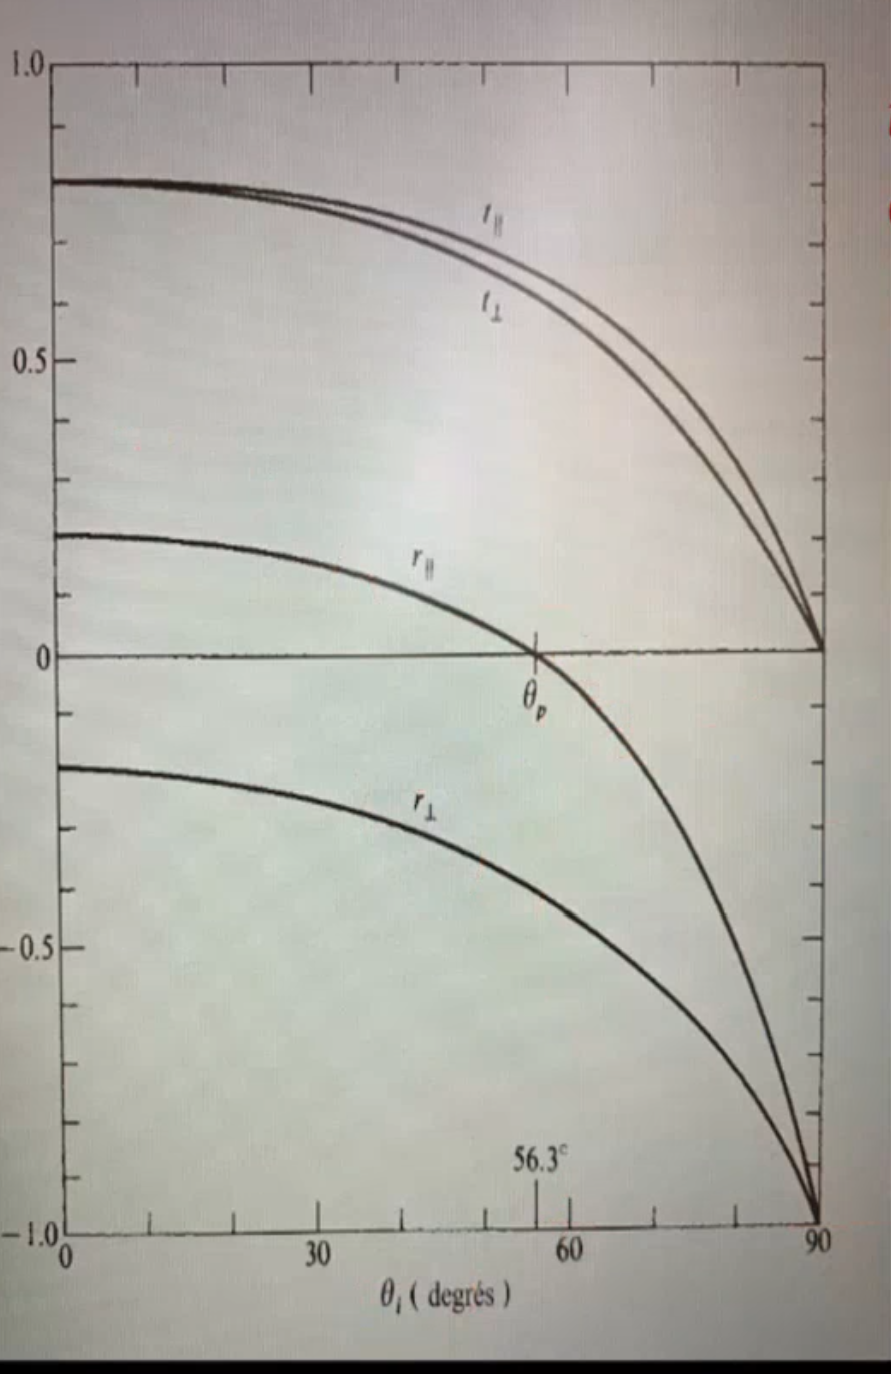
\includegraphics[width =\linewidth]{pic/graphe1.png}
                    \end{minipage}
                    \begin{minipage}{0.49\linewidth}
                        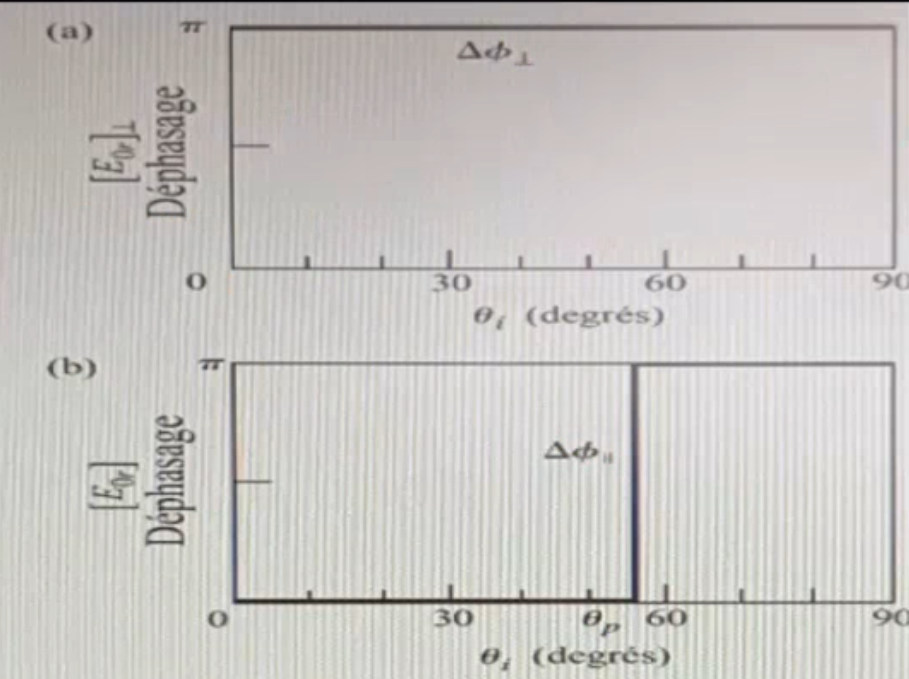
\includegraphics[width = \linewidth]{pic/graphe2.png}
                    \end{minipage}
                \end{center}
            \underline{$n_t < n_i$} 
                \begin{center}
                    \begin{minipage}{0.3\linewidth}
                        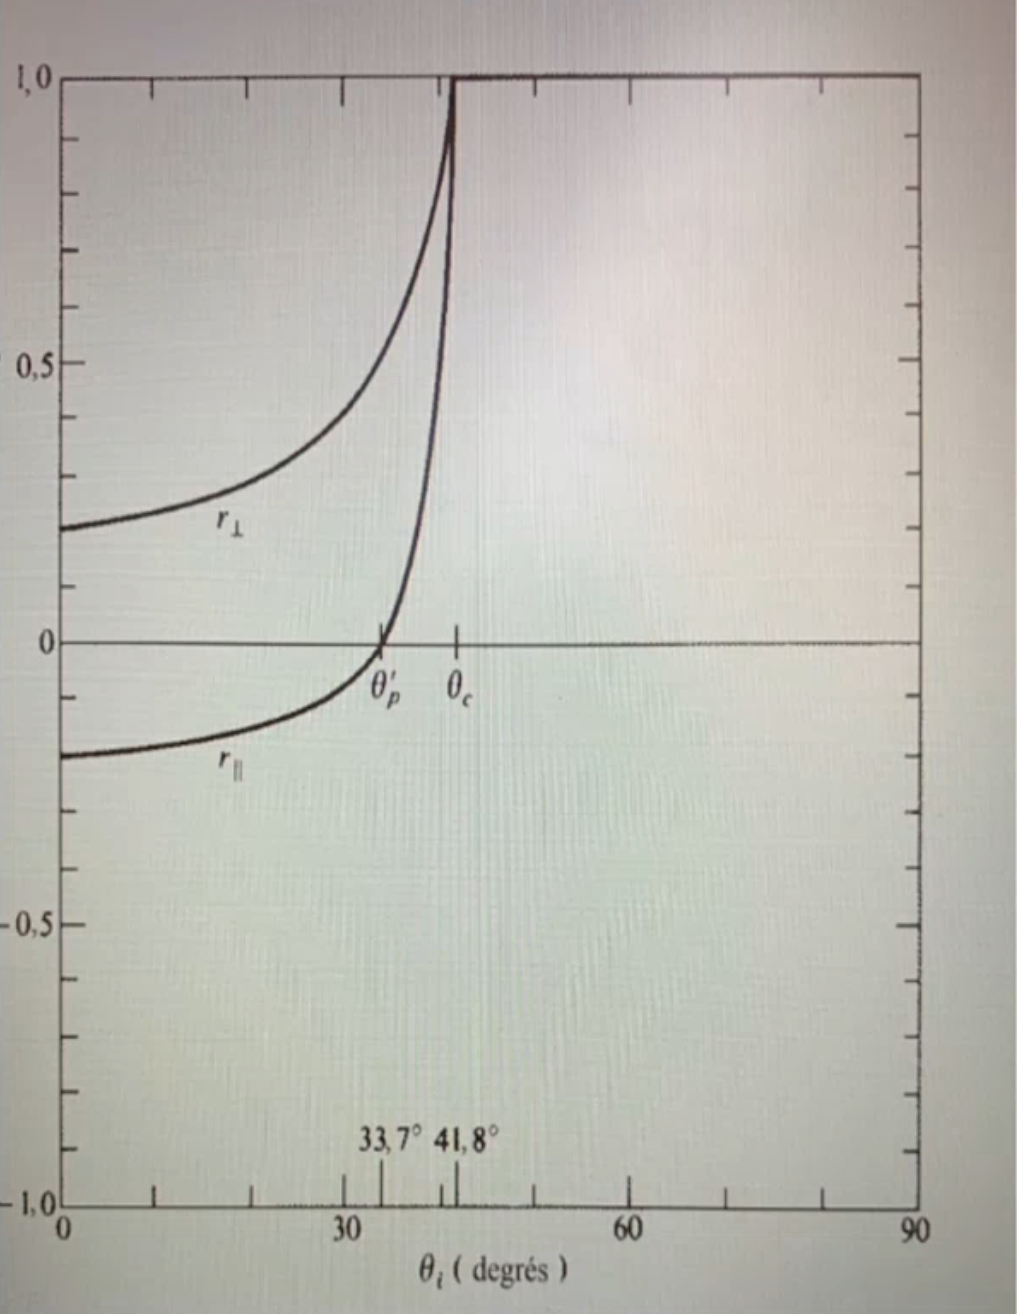
\includegraphics[width =\linewidth]{pic/graphe3.png}
                    \end{minipage}
                    \begin{minipage}{0.49\linewidth}
                        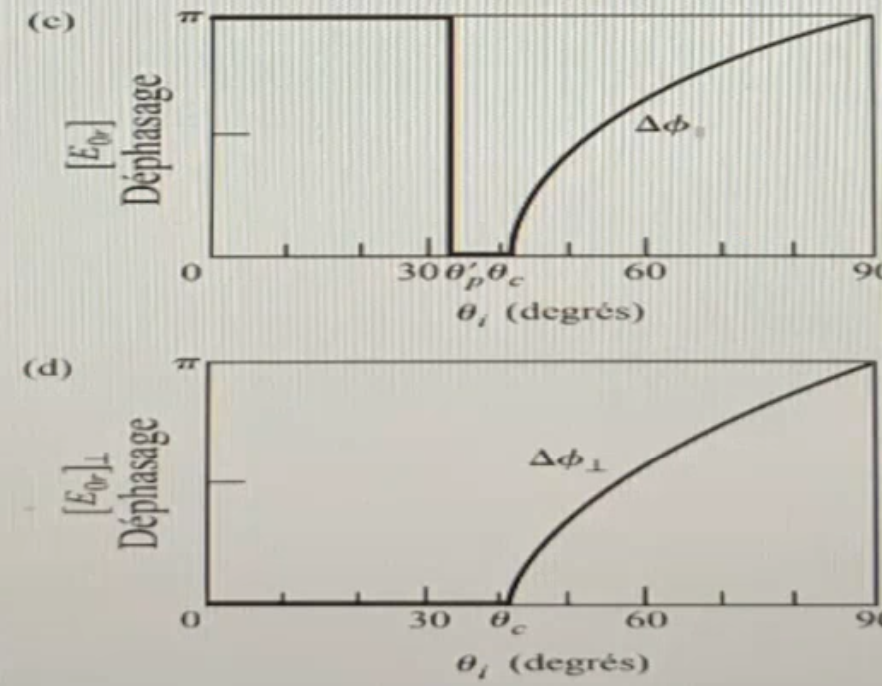
\includegraphics[width = \linewidth]{pic/graphe4.png}
                    \end{minipage}
                \end{center}
        \section{Coefficient de reflexion et transmission relatif aux intensite}
            On definit les facteur de reflexion ($R$) et de Transmission ($T$) relatif aux pussiance ( ou intensite) 
            \begin{center}
                $R = \frac{\langle P_r \rangle}{\langle P_i \rangle}$ , 
                $T = \frac{\langle P_t \rangle}{\langle P_i \rangle}$
            \end{center}
            avec $\langle P \rangle = \iint \vec{S}.d\vec{s} =\langle \vec{S} \rangle .\vv{s} $ ou $\langle \vec{S} \rangle = \langle \frac{1}{\mu}\vec{E}\wedge\vec{B} \rangle $ \\
            Champ electrique
            \begin{itemize}
                \item $\vv{E_i} = \vv{u_z}A_i\cos(wt-\vv{k_i}\vv{i})$
                \item $\vv{E_r} = \vv{u_z}A_r\cos(wt-\vv{k_r}\vv{r})$
                \item $\vv{E_t} = \vv{u_z}A_t\cos(wt-\vv{k_t}\vv{t})$
            \end{itemize}
            Champ magnetique
            \begin{itemize}
                \item $\vv{B_i} = (-\cos(\theta_i)\vv{u_x} - \sin(\theta_i)\vv{u_y})\frac{A_i}{v_1}\cos(wt - \vv{k_i}\vv{r})$
                \item $\vv{B_r} = (\cos(\theta_i)\vv{u_x} - \sin(\theta_i)\vv{u_y})\frac{A_r}{v_1}\cos(wt - \vv{k_r}\vv{r})$
                \item $\vv{B_t} = (-\cos(\theta_i)\vv{u_x} - \sin(\theta_i)\vv{u_y})\frac{A_t}{v_2}\cos(wt - \vv{k_t}\vv{r})$
            \end{itemize}
            Densite moyen du puissance
            \begin{itemize}
                \item $\langle \vv{S_i} \rangle = \langle \frac{1}{\mu_1}\frac{A_i^2}{v_1} \cos(k_i\vv{r} - wt) \rangle\vv{u_i} = \frac{1}{2\mu_1}\frac{A_i^2}{v_1}\vv{u_i} $
                \item $\langle \vv{S_r} \rangle = \langle \frac{1}{\mu_1}\frac{A_r^2}{v_1} \cos(k_r\vv{r} - wt) \rangle\vv{u_r} = \frac{1}{2\mu_1}\frac{A_r^2}{v_1}\vv{u_r} $
                \item $\langle \vv{S_t} \rangle = \langle \frac{1}{\mu_2}\frac{A_t^2}{v_2} \cos(k_t\vv{r} - wt) \rangle\vv{u_t} = \frac{1}{2\mu_2}\frac{A_t^2}{v_2}\vv{u_t} $
            \end{itemize}
            Puissance moyen
            \begin{itemize}
                \item $\langle P_i \rangle = \frac{1}{2\mu_1}\frac{A_i^2}{v_1}\cos(\theta_i)s= I_i\cos(\theta_i)s $
                \item $\langle P_r \rangle = \frac{1}{2\mu_1}\frac{A_r^2}{v_1}\cos(\theta_i)s= I_r\cos(\theta_i)s $
                \item $\langle P_t \rangle = \frac{1}{2\mu_2}\frac{A_t^2}{v_2}\cos(\theta_i)s= I_t\cos(\theta_i)s $
            \end{itemize}
                \begin{center}
                    Coefficient de Reflexion
                \end{center}
                \begin{itemize}
                    \item 
                        \begin{center}
                            \boxed{R_\perp = \frac{\langle P_{r_\perp} \rangle}{\langle P_{i_\perp} \rangle} = \left( \frac{A_{r_\perp}}{A_{i_\perp}}\right)^2 = r_\perp^2 }
                        \end{center}
                    \item 
                    \begin{center}
                        \boxed{R_\parallel = \frac{\langle P_{r_\parallel} \rangle}{\langle P_{i_\parallel} \rangle} = \left( \frac{A_{r_\parallel}}{A_{i_\parallel}}\right)^2 = r_\parallel^2 }
                    \end{center}
                \end{itemize}
                \begin{center}
                    Coefficient de Transmission
                \end{center}
                \begin{itemize}
                    \item 
                        \begin{center}
                            \boxed{T_\perp = \frac{\langle P_{t_\perp} \rangle}{\langle P_{i_\perp} \rangle} = \frac{\cos(\theta_t)}{\cos(\theta_i)} \left( \frac{A_{r_\perp}}{A_{i_\perp}}\right)^2 \frac{v_1}{v_2} = \frac{\cos(\theta_t)}{\cos(\theta_i)} \frac{n_t}{n_i}t_\perp^2 }
                        \end{center}
                    \item 
                        \begin{center}
                            \boxed{T_\parallel = \frac{\langle P_{t_\parallel} \rangle}{\langle P_{i_\parallel} \rangle} = \frac{\cos(\theta_t)}{\cos(\theta_i)} \left( \frac{A_{r_\parallel}}{A_{i_\parallel}}\right)^2 \frac{v_1}{v_2} = \frac{\cos(\theta_t)}{\cos(\theta_i)} \frac{n_t}{n_i}t_\parallel^2 }
                        \end{center}
                
                \end{itemize}
                \underline{Relation :} \boxed{R_\perp^\parallel+T_\perp^\parallel =1}
    \chapter{Method matricielle de Propagation }
        \subsection{Introduction}
            \begin{itemize}
                \item La method optique matricielle permet determiner travers des matrices $2 \times 2$ , tous les caracterisiques liees a la propagatin de la lumiere entre l objet e l image
                \item le principe de cette methode consist a associer a chaque partie optique du traget lumineux entre l objet et l image une matrice specifique ($2 \times 2$) caractersant cette partie optique par simple multiplication de tous les matrices qui represent ces partie , on peut determiner les caracteristique liees a la propagation depuis l objet jusqu'a l image 
                \item tout rayon est caracterise par sa hauteur y et par son angle d inclinaison $\theta$ 
                  
            \end{itemize}
        \subsection{Condition de Gaus}
            \begin{itemize}
                \item  System optique center
                \item $\theta \cong \sin(\theta) \cong \tan(\theta)$ (car $\theta $ est faible)
                \item Grandissement transversal $G_+ = \frac{\overline{A_2B_2}}{\overline{A_1B_1}}$
                \item Grandissement angulair $G_a = \frac{\alpha_2}{\alpha_1}$ (par raport a laxe optique)\\
                    \begin{center}
                        \boxed{\frac{n_2}{n_1}G_tG_a =1}
                    \end{center}
                \item  les point H et S sont presque confondu \\ \begin{center}
                    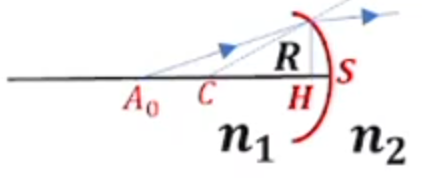
\includegraphics[width = 0.2\linewidth]{pic/HetSconfoundu.png}
                \end{center}
                \item la vergence d' un dioptre spherique \boxed{v= \frac{n_2 - n_1}{R}} avec $R < 0 $ ou $ R >0$ 
                \begin{center}
                    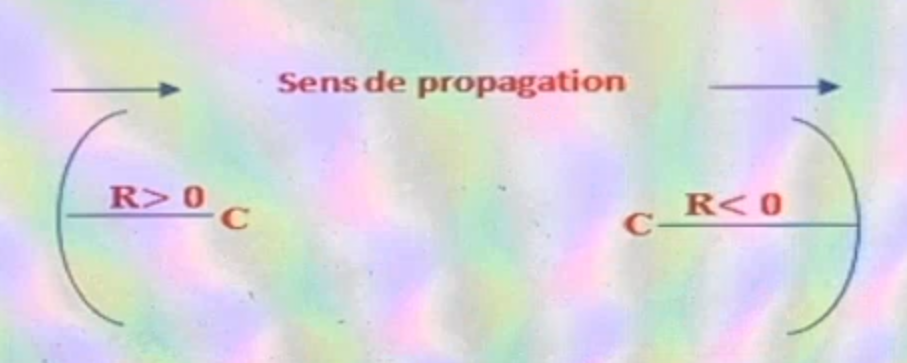
\includegraphics[width = 0.4\linewidth]{pic/Rposnega.png}
                \end{center}
            \end{itemize}
        \subsection{La method matricielle}
            \begin{center}
                \boxed{
                    \begin{pmatrix}
                        h_2\\
                        n_2\theta_2
                    \end{pmatrix}
                    = \begin{pmatrix}
                        A & B \\
                        C & D 
                    \end{pmatrix}
                    \begin{pmatrix}
                        h_1\\
                        n_1\theta_1
                    \end{pmatrix}
                } \\
                Matrice image = Matrice transfert $\times$ Matrice objet \\ 
                $ \implies$\boxed{ h_2 = Ah_1 + Bn_1\theta_1 } et \boxed{n_2\theta_2 = Ch_1 + Dn_1\theta_1} \\
                A , B < C et D sont fonctions des partie optique qu'ils represent

            \end{center}
        \subsection{Propagation libre dans un milieu d indicec $n$}
            \begin{center}
                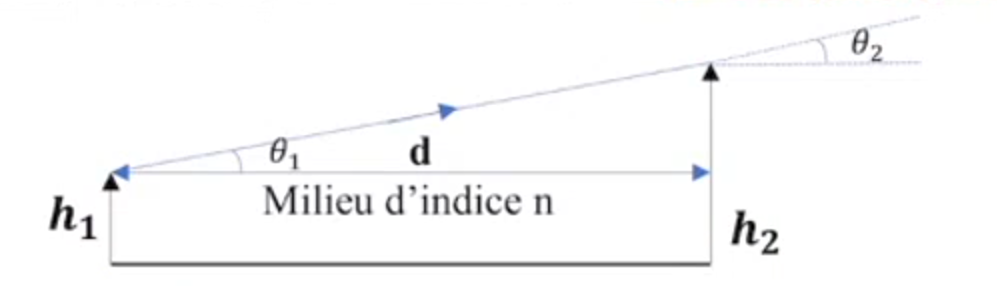
\includegraphics[width = 0.5\linewidth]{pic/proplibre.png}
            \end{center}
            ona dans ce cas:
            \begin{itemize}
                \item $n_1 = n_2$(la lumiere propage dans lameme milieu)
                \item $\theta_1 = \theta_2$ ( la lumiere na pas subit une deviation par obstacle)
                \item $\theta_1 \cong \tan(\theta_1) = \frac{h_2 - h_1}{d} \implies h_2 - h_1 = \theta_1d \implies h_2 =h_1 + d\theta_1$ 
            \end{itemize}
            ona toujour :
            \begin{itemize}
                \item $ h_2 = Ah_1 + Bn_1\theta_1$
                \item $ n_2\theta_2 = Ch_1 + Dn_1\theta_1$
            \end{itemize}
            alors : $ A = 1 , B = \frac{d}{n} ,C = 0 , D = 1$ \\ 
            matrice de transfert : 
            \begin{center}
                \boxed{
                    T_{propagation \; libre}= \begin{pmatrix}
                        1 & \frac{d}{n} \\
                        0 & 1 
                    \end{pmatrix}
                } \\
            \end{center}
        \subsection{Refraction sur un dioptre plan}
            \begin{center}
                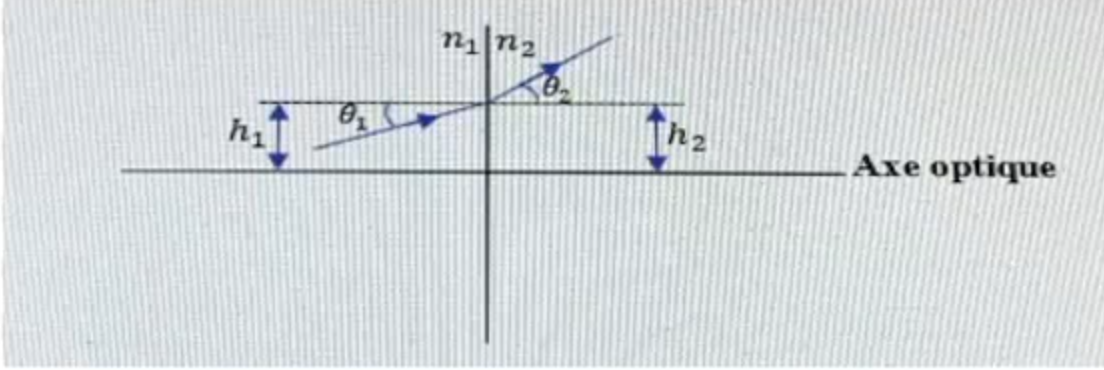
\includegraphics[width = 0.5\linewidth]{pic/dioptreplan.png}
            \end{center}
            \begin{center}
                \begin{minipage}{0.49\linewidth}
                    ona dans ce cas:
                    \begin{itemize}
                        \item $n_1\theta_1 = n_2\theta_2$
                        \item $h_1 = h_2$
                    \end{itemize}
                    
                \end{minipage}
                \begin{minipage}{0.49\linewidth}
                    ona toujour :
                    \begin{itemize}
                        \item $ h_2 = Ah_1 + Bn_1\theta_1$
                        \item $ n_2\theta_2 = Ch_1 + Dn_1\theta_1$
                    \end{itemize}
                    
                \end{minipage}
            \end{center}
            alors : $ A = 1 , B = 0 ,C = 0 , D = 1$ \\ 
            matrice de transfert : 
            \begin{center}
                \boxed{
                    T_{dioptre \; plan}= \begin{pmatrix}
                        1 & 0 \\
                        0 & 1 
                    \end{pmatrix}
                } 
            \end{center}
            
        \subsection{Refraction sur un dioptre spherique}
            \begin{center}
                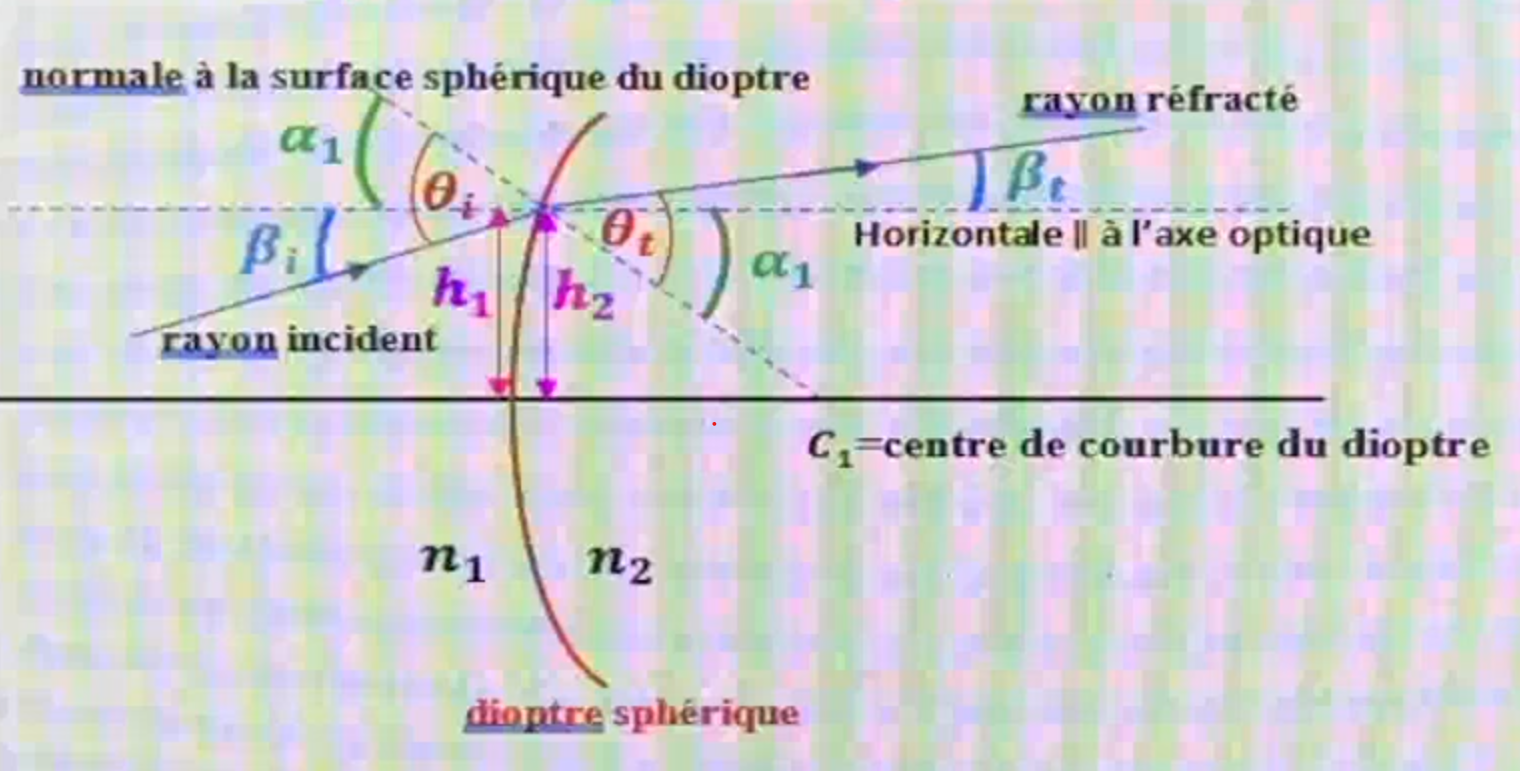
\includegraphics[width = 0.6\linewidth]{pic/dioptrespherique.png}
            \end{center}
            ona dans ce cas:
            \begin{itemize}
                \item $n_1\theta_1 = n_2\theta_2$
                \item $h_1 = h_2$
                \item $\theta_i =\beta_i + \alpha_1$ et $\theta_t =\beta_t + \alpha_1 \implies n_1(\beta_i + \alpha_1) = n_2(\beta_t + \alpha_1)  $ \\ 
                      $\implies n_2\beta_t = n_1\beta_i +n_1\alpha_1 - n_2\alpha_1$ \\
                      $\tan(\alpha_1) = \alpha_1 = \frac{h_1}{R_1} \implies n_2\beta_t = n_1\beta_i +n_1\frac{h_1}{R_1} - n_2\frac{h_1}{R_1} \implies \ldots \implies $ \\
                      \boxed{n_2\beta_t = n_1\beta_i - h_1V_1} avec $V_1 = (\frac{n_2-n_1}{R_1}) = \frac{1}{f_1}$ (Vergence du dioptre)
            \end{itemize}
            \pagebreak
            ona toujour :
            \begin{itemize}
                \item $ h_2 = Ah_1 + Bn_1\theta_1$
                \item $ n_2\theta_2 = Ch_1 + Dn_1\theta_1$
            \end{itemize}
            alors : $ A = 1 , B = 0 ,C = 1 , D = -V_1$ \\ 
            matrice de transfert : 
            \begin{center}
                \boxed{
                    T_{dioptre \; spherique}= \begin{pmatrix}
                        1 & 0 \\
                        -V_1& 1
                    \end{pmatrix}
                } \\
            \end{center}
        
        \subsection{Traverse d 'une lentille epaisse}
            \begin{center}
                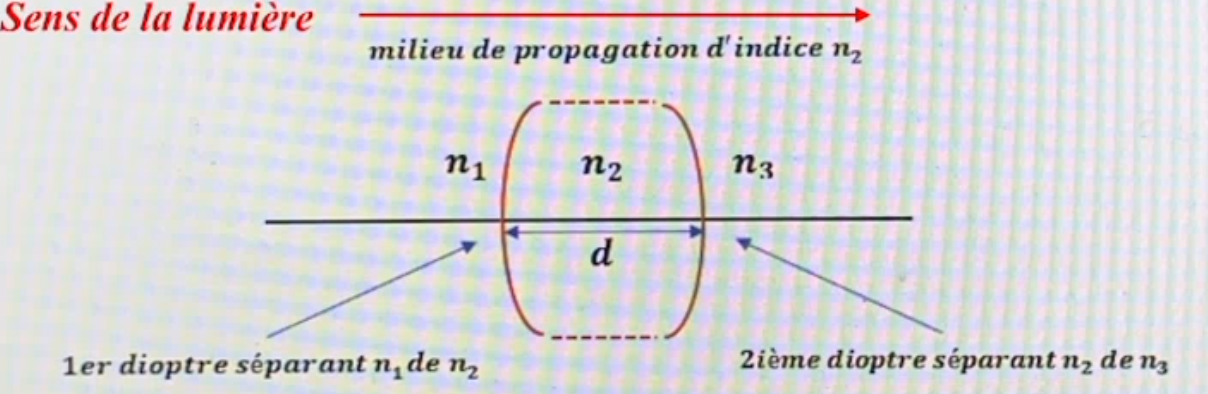
\includegraphics[width = 0.6\linewidth]{pic/lentilleepaisse.png}
            \end{center}
            Une lentille epaisse est une association de deux dioptre spherique et d'une propagation libre  \\
            alor le matrice de transfert est la  multiplication des matrices (2em dioptre , propagation libre , 1er dioptre)
            \\
            matrice de transfert : 
            $
            T_{lentille \; epaisse}= 
            \begin{pmatrix}
                1 & 0 \\
                -V_2& -0
            \end{pmatrix} \times
            \begin{pmatrix}
                1 & \frac{d}{n_2}\\
                0 & 1
            \end{pmatrix} \times
            \begin{pmatrix}
                1 & 0 \\
                -V_1& -0
            \end{pmatrix}
            $          
            \begin{center}
                \boxed{
                    T_{lentille \; epaisse}= 
                    \begin{pmatrix}
                        1-V_1\frac{d}{n_2} & \frac{d}{n_2} \\
                        -V_1-V_2 + V_1V_2\frac{d}{n_2} & 1-V_1\frac{d}{n_2}
                    \end{pmatrix}
                } \\ avec $V_1 = (\frac{n_2 - n_1}{R_1})$ et $V_2 = (\frac{n_3 - n_2}{R_2})$
            \end{center} 
        \subsection{Traverse d'une lentille mince}
            la lentille mince est un cas particuliair du lentille epaisse ou $d=0$
            \\ matrice de transfer :
            \begin{center}
                \boxed{
                    T_{lentille \; mince}= 
                    \begin{pmatrix}
                        1 & 0\\
                        -V_1-V_2 & 1
                    \end{pmatrix}
                } \\ avec $V_1 = (\frac{n_2 - n_1}{R_1})$ et $V_2 = (\frac{n_3 - n_2}{R_2})$
            \end{center} 
        \subsection{Reflexion sur un miroir}
            matrice de transfer :
            \begin{center}
                \boxed{
                    T_{miroir}= 
                    \begin{pmatrix}
                        1 & 0\\
                    \frac{-2}{R}n & -1
                    \end{pmatrix}
                } \\ dans le cas d 'une miroire plan $R \to \infty$
            \end{center} 
    \section{Cavite optique}
        \begin{itemize}
            \item Une cavite est un montage constitue generalement de miroirs , lentilles et de propagation libre , dans laquelle le tayon lumineux se trouve confine dans le montage et ne sort plusieur
            \item Si le rayon retrouve son etat de depart (hauteur et inclinaison) apres un certaine combre de aller-retour dans se cas la cavite est periodique \\
                  Cette periodicite s'exprime par la relation :
                  \begin{center}
                    \boxed{y_n = y_{max}\sin(m_\phi + \phi_0)} \\
                    $\phi = \frac{\pi}{n}$ ou $n\pi$ ( $n$ est un nombre entier)
                  \end{center}
                  avec : 
                  \begin{itemize}
                    \item $y_n$ : hauteur de rayon par rapport a l'axe optique apres $(m)$ allers-retours
                    \item $y_max$ : hauteur maximale atteinte suite a ces $(m)$ allers-retours 
                    \item $\cos(\phi) = \frac{A+D}{2}$
                    \item $\tan(\phi_0) = \frac{y_0\sqrt{1+(\frac{A+D}{2})^2}}{y_0 \sqrt{(\frac{A-D}{2})+B\theta_0}}$
                    \item $\theta_0 $ : inclinaison initiale (a $(0)$ aller-retour ) 
                    \item $y_0 = y_{max}\sin(\phi_0) $ : hauteur initiale (a $(0)$ aller-retour ) 
                  \end{itemize}
            \item quand le rayon reste dans la cavite et ne diverge pas vers l'exterieur , la cavite est stable
             \\   ceci arrive si : $-1 \leq \frac{A+D}{2}\leq 1 $ ou bien $0 \leq \frac{A+D+2}{4}\leq 1 $ \\
             avec $A$ et $D$ sont les termes de la matrice 
             $\begin{pmatrix}
                A & B\\
                C & D
            \end{pmatrix}$
            qui represente la cavite 
        \end{itemize}
        \pagebreak
        \subsection{Cellue unite de la cavite optique}
        Chaque cavite optique a une cellule unite qui se repet pendant le trajet lumineux .\\
        Pour la determiner il faut trouver le montage optique equivalent a notre cavite en remplacent les miroire en reflexin par leurs equivalent en transmission
        \begin{itemize}
            \item Pour replacer un miroir \underline{plan} en mode transmission il suffit de deplier le trajet lumineux
               \\ 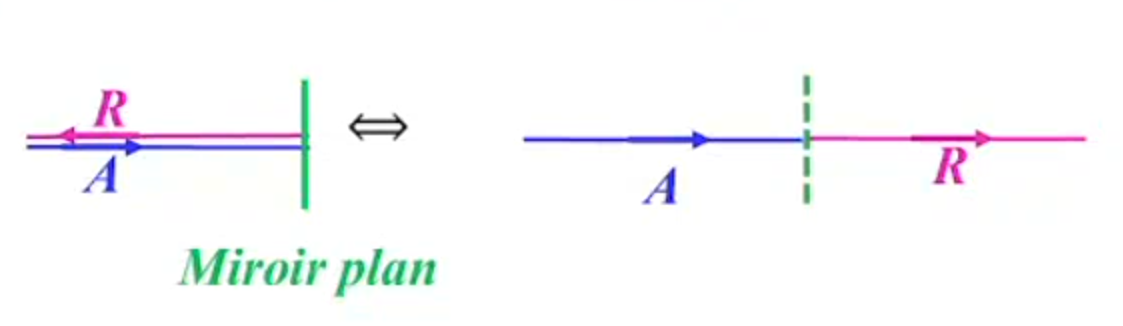
\includegraphics[width = 0.6\linewidth]{pic/celluleplan.png}
            \item Pour replacer un miroir \underline{spherique concave } en mode transmission il de remplacer par une \underline{lentille mince convergent}
              \\  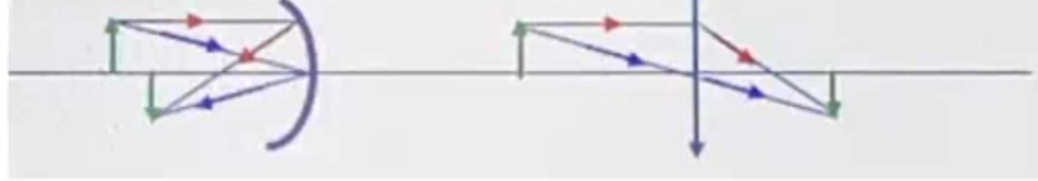
\includegraphics[width = 0.6\linewidth]{pic/celluleconcave.png}
            \item Pour replacer un miroir \underline{spherique convexe } en mode transmission il de remplacer par une \underline{lentille mince divergente}
               \\ 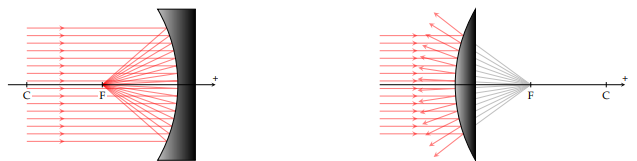
\includegraphics[width = 0.6\linewidth]{pic/celluleconvexe.png}
        \end{itemize}
    \chapter{Les phenomenes d interference}
        \section{definition}
            \begin{itemize}
                \item le phenomen d interfernce result de la superposition entre deux ou plusieur onde lumineuses
                \item pour ce phenomen soit possible il faut que les ondes qui se superposent soient
                    \begin{itemize}
                        \item coherentes spatialement
                            si les phases des ondes qui se superposent sont les mem a tout instant \\
                            \\ \underline{Note :} le coherence spatiale est n est pas posible si les sources des ondes sont independantes
                        \item coherantes temporellement
                            si les ondes que se superposent on exactement le meme frequence
                \end{itemize}
            \end{itemize}
        \section{Expression mathematique de phenomen d interference entre deux ondes}
            \begin{itemize}
                \item Soi deux ondes planes coherentes temporellement (meme $w$) et spatialement (meme phase) qui se superposent en un point $M$ de l'espace. Ce point $M$ est situe a une postion $ \vv{r_1}$ de $S_1$ et $\vv{r_2}$ de $S2$ \\
                    les champs electriques deces ondes s'ecrivent : $\begin{cases}
                        \vv{E_1} = \vv{E_{01}}\cos(\vv{k_1}\vv{r_1}-wt)\\
                        \vv{E_2} = \vv{E_{02}}\cos(\vv{k_2}\vv{r_2}-wt)
                    \end{cases}$  \\
                \item En interference on s'interesse a l'intensite lumineuse $I = | \langle \vv{S}\rangle |$ avec :
                    $\vv{S} =\vv{\boldsymbol{S}}=\frac{1}{\mu} \vv{\boldsymbol{E}} \wedge \vv{\boldsymbol{B}}=\frac{1}{\mu} \boldsymbol{E} B \sin \frac{\pi}{2} \vv{\boldsymbol{u}}=\frac{1}{\mu v} E^{2} \vv{\boldsymbol{u}}=\frac{\varepsilon v^{2}}{v} E^{2} \vec{u}=\varepsilon v E^{2} \vv{\boldsymbol{u}}\langle\vv{\boldsymbol{S}}\rangle=\varepsilon v\left\langle E^{2}\right\rangle \vv{\boldsymbol{u}} \implies$
                    \begin{center}
                        \boxed{I=|\langle\vec{S}\rangle|=\varepsilon v\left\langle E^{2}\right\rangle \implies I \equiv \langle E^2 \rangle}\\
                        $ I \equiv \langle E^2 \rangle$ car l intensite depend de champ electrique et $\varepsilon v$ sont des constant \\ (l identite et les caracteristique de l intensite est dans la valeur de $E$)  
                    \end{center} 
                \item On a $\vv{E} =\vv{E_1} + \vv{E_2} \implies \vv{E^2}=(\vv{E_1}+\vv{E_2})(\vv{E_1}+\vv{E_2})=\vv{E_1^2}+\vv{E_2^2}+2\vv{E_1}\vv{E_2}$\\
                    et $ I \equiv \langle E^2 \rangle$ $\implies $ \boxed{I=I_1+I_2+2\underbrace{I_{12}}}($I_{12}$ est le terme d'interferance)
                \item $I_{12} = \langle \vv{E_1}\vv{E_2} \rangle $ et $ \vv{E_1}\vv{E_2} =\vv{E_{01}}\vv{E_{02}}\cos(\vv{k_1}\vv{r_1}-wt)\cos(\vv{k_2}\vv{r_2}-wt)$\\
                    avec $\begin{cases}
                        \cos(\vv{k_1}\vv{r_1}-wt) = \cos(\vv{k_1}\vv{r_1})\cos(wt)+\sin(\vv{k_1}\vv{r_1})\sin(wt)          \\                        
                        \cos(\vv{k_2}\vv{r_2}-wt) = \cos(\vv{k_2}\vv{r_2})\cos(wt)+\sin(\vv{k_2}\vv{r_2})\sin(wt)                                  
                        \end{cases}$ \\
                    $\implies \vv{E}_{1}  \vv{E}_{2}=\vv{E}_{01}  \vv{E}_{02}\left[\cos \left(\vv{k}_{1}  \vv{r}_{1}\right) \cos \left(\vv{k}_{2}  \vv{r}_{2}\right) \cos ^{2} w t \right. \\ \left. +  \sin \left(\vv{k}_{1}  \vv{r}_{1}\right) \sin \left(\vv{k}_{2}  \vv{r}_{2}\right) \sin 2 w t  +\cos \left(\vv{k}_{1}  \vv{r}_{1}\right) \sin \left(\vv{k}_{2}  \vv{r}_{2}\right) \cos w t \sin w t+ \right. \\ \left.\cos \left(\vv{k}_{2}  \vv{r}_{2}\right) \sin \left(\vv{k}_{1}  \vv{r}_{2}\right) \cos w t \sin w t\right]$
                    \\ $\implies \left\langle\vv{E}_{1}  \vv{E}_{2}\right\rangle=\vv{E}_{01}  \vv{E}_{02}\left[\left\langle\cos \left(\vv{k}_{1}  \vv{r}_{1}\right) \cos \left(\vv{k}_{2}  \vv{r}_{2}\right) \cos ^{2} w t\right\rangle \right. \\ \left. +\left\langle\sin \left(\vv{k}_{1}  \vv{r}_{1}\right) \sin \left(\vv{k}_{2}  \vv{r}_{2}\right) \sin 2 w t\right\rangle+\left\langle\cos \left(\vv{k}_{1}  \vv{r}_{1}\right) \sin \left(\vv{k}_{2}  \vv{r}_{2}\right) \cos w t \sin w t\right\rangle \right. \\ \left.+\left\langle\cos \left(\vv{k}_{2}  \vv{r}_{2}\right) \sin \left(\vv{k}_{1}  \vv{r}_{1}\right) \cos w t \sin w t\right\rangle\right]$
                    \\ $\implies \langle \vv{E_1}\vv{E_2} \rangle =\vv{E_{01}}\vv{E_{02}}\left[ \frac{1}{2}\cos(\vv{k_1}\vv{r_1})\cos(\vv{k_2}\vv{r_2})+\frac{1}{2}\sin(\vv{k_1}\vv{r_1})\sin(\vv{k_2}\vv{r_2})+0 +0 \right] $\\
                    $\implies \langle \vv{E_1}\vv{E_2} \rangle = \vv{E_{01}}\vv{E_{02}}\frac{1}{2}\cos\left[ (\vv{k_1}\vv{r_1}) - (\vv{k_2}\vv{r_2}) \right]$ \\
                    Soit $\vv{k_1}\vv{r_1} - \vv{k_2}\vv{r_2} = \Delta\phi$ Alors \boxed{I_{12} =  \langle \vv{E_1}\vv{E_2} \rangle = \vv{E_{01}}\vv{E_{02}}\frac{1}{2}\cos(\Delta\phi)}\\ 
                    \underline{Note :} le moyen de cosinus et le moyen de sinus est $0$ , le moyen de sinus caree et cosinus caree est $\frac{1}{2}$
                \item $\begin{cases}
                    I_1 = \langle \vv{E_1^2 }\rangle = \langle \vv{E_{01}}\cos(\vv{k_1}\vv{r_1} -wt)\vv{E_{01}}\cos(\vv{k_1}\vv{r_1}-wt) \rangle =\frac{1}{2}\vv{E_{01}^2}\\
                    I_2  = \langle \vv{E_2^2 }\rangle = \langle \vv{E_{02}}\cos(\vv{k_2}\vv{r_2} -wt)\vv{E_{02}}\cos(\vv{k_2}\vv{r_2}-wt) \rangle =\frac{1}{2}\vv{E_{02}^2}
                    \end{cases}$\\
                    Alors \boxed{E_{01} = \sqrt{2I_1}} et \boxed{E_{02} = \sqrt{2I_2}}
                \item  $I_{12}=\frac{1}{2}\vv{E_{01}}\vv{E_{02}}\cos(\Delta\phi) \implies $\boxed{I_{12} = \sqrt{I_1I_2}\cos(\Delta\phi) }
                \item  En fin : \begin{center}
                    \boxed{I=I_1+I_2+2\sqrt{I_1I_2}\cos(\Delta\phi)} avec $\Delta\phi = \vv{k_1}\vv{r_1} - \vv{k_2}\vv{r_2} $
                \end{center}
            \end{itemize}
            \subsection*{Interference constructive}
                $I_{max} \implies \cos(\Delta\phi) = 1 = \cos(2m\pi)\implies$\boxed{\Delta\phi=2m\pi}$\implies$\boxed{I_{max}=(\sqrt{I_1}+\sqrt{I_2})^2}\\
            \subsection*{Interference destructive}
                $I_{max} \implies \cos(\Delta\phi) = -1 = \cos((2m+1)\pi)\implies$\boxed{\Delta\phi=(2m+1)\pi}$\implies$\boxed{I_{max}=(\sqrt{I_1}-\sqrt{I_2})^2}\\
            \subsection*{Si $E_{01} = E_{02}$}
                \begin{center}
                    \begin{minipage}{0.49\linewidth}
                        $ I_1=I_2=I_0 \implies 2I_0(2\cos^2(\frac{\Delta\phi}{2})) \\ \implies$ 
                        \boxed{I=4I_0\cos^2(\frac{\Delta\phi}{2})}$\begin{cases}
                            I_{max}=4I_0\\
                            I_{min}=0\\
                        \end{cases}$
                    \end{minipage}
                    \begin{minipage}{0.49\linewidth}
                        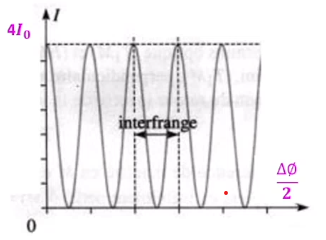
\includegraphics[width=\linewidth]{pic/interference.png}                      
                    \end{minipage}
                \end{center}
        \section{Dispositifs d'Young}
            \begin{center}
                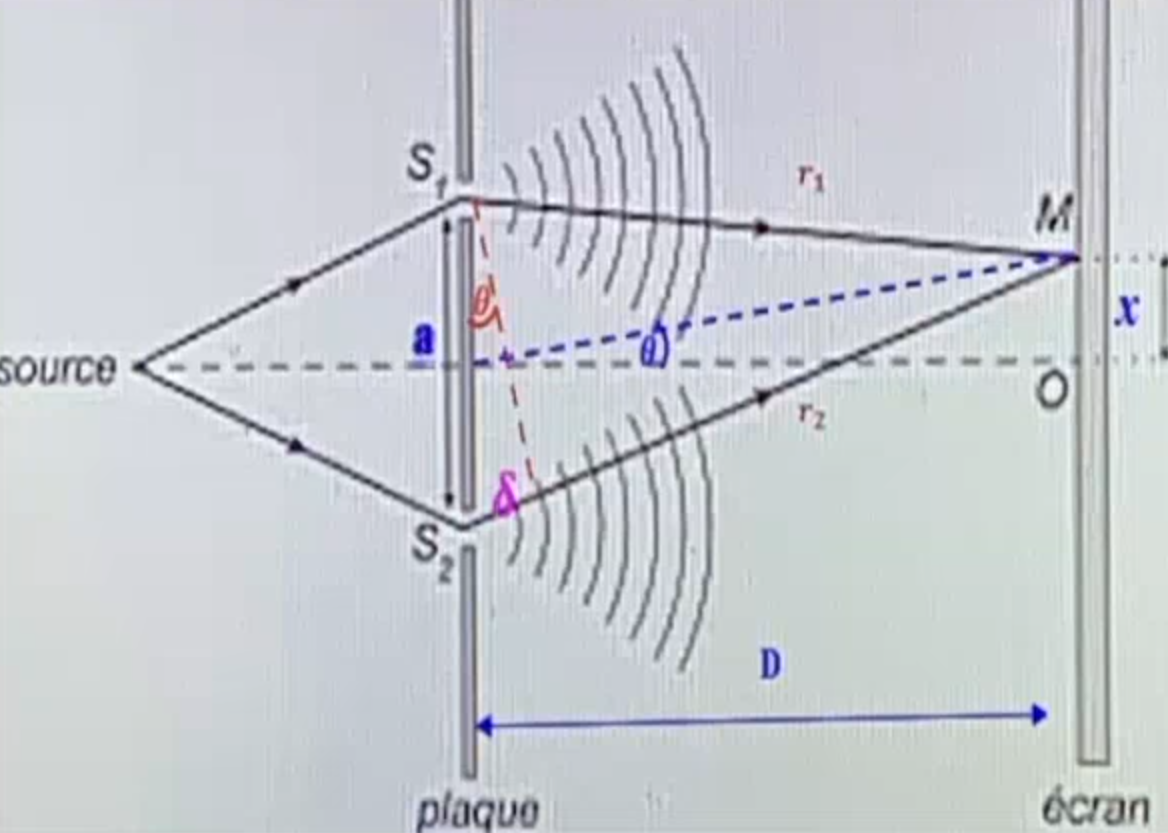
\includegraphics[width=0.3\linewidth]{pic/young.png}
            \end{center}
            \begin{itemize}
               \item Description \\
                    \begin{itemize}
                        \item Une source $(S)$ de lumieure monochromatique eclaire un ecran muni de deux fentes identiques $(S_1)$ et $(S_2)$ distantes de $a$
                        \item la lumiere est diffractee par $(S_1)$ et $(S_2)$ pour subir un phenomene d'interfernece en un point $M$ sur un ecran situe a une distance $D$ du plan de $(S_1)$ et $(S_2)$ 
                        \item $(S_1)$ et $(S_2)$ sont deux sources secondaires \underline{coherents} car issues d'une meme source monochromatique (Laser)
                        \item $M$ se trouve a une distance $r_1$ de $(S_1)$ et $r_2$ de $(S_2)$
                        \item Le Dispositifs d'Young est un interferometre a division du front d'onde car le fron d'onde de $(S)$ est divise en deux fronts d'onde a partir $(S_1)$ et $(S_2)$
                        \item les deux sources sont identique $(S_1)$ et $(S_2) \\
                         \implies  E_{01}=E_{02} \implies$\boxed{ I = 4I_0\cos^2(\frac{\Delta\phi}{2})
                         \begin{cases}
                             I_{max} \implies \Delta\phi =2m\pi \\
                             I_{min} \implies \Delta\phi =(2m +1)\pi
                         \end{cases}}
                        \item $(S_1)$ et $(S_2)$ emettent deux ondes spheriques secondaires identiques \\ $\implies $ \boxed{\vv{k_1}\vv{r_1}=k_1r_1} et \boxed{\vv{k_2}\vv{r_2}=k_2r_2} 
                    \end{itemize}
                \item Si les ondes se propagent dans le meme milieu alors $k_1 = k_2=\frac{2\pi}{\lambda} \\ \implies $\boxed{\Delta\phi = k(r_2-r_1) = \frac{2\pi}{\lambda}\delta = \frac{2\pi}{\lambda_0}n\delta=\frac{2\pi}{\lambda_0}\delta^{'}}
                    \begin{itemize}
                        \item \boxed{\delta = (r_2 - r_1)}$ = $ difference de marche $=$ parcours supplementaire de (2) relativement a (1) 
                        \item \boxed{\delta^{'} = n\delta} = difference de marche optique 
                        \item $\lambda_0 =$ longeur d onde dan l'air 
                        \item $\lambda = $longueur d'onde dans le milieu d'indice $n$
                    \end{itemize}
                \item interference constructive \\
                    $\implies I_{max}\implies\Delta\phi=2m\pi=k\delta=\frac{2\pi}{\lambda}\alpha\implies$\boxed{\delta=m\lambda}
                \item interference destuctive \\
                     $\implies I_{min}\implies\Delta\phi=(2m+1)\pi=k\delta=\frac{2\pi}{\lambda}\alpha\implies$\boxed{\delta=(2m+1)\frac{\lambda}{2}}
                \item Un dephasage $\Delta\phi\text{ de }\pi$ correspond donc a une differnce de marche $\delta$ de $\frac{\lambda}{2}$
                \item Si $\delta = m\lambda \implies $ les deux ondes sont en phase \\
                    $m=0 \implies$ Frange Centrale Brilliante (frange d'ordre 0) \\
                    $m = \pm 1 , \pm 2 , \ldots \implies $ Franges Brilliantees d 'ordre 1,2,\ldots
                \item Si $\delta = (2m+1)\frac{\lambda}{2} \implies $ les deux ondes sont en opposition de phase \\
                    $m = 0 ,\pm1 ,\pm2 \ldots \implies$ Franges sombres d'ordre 0,1,2,\ldots 
                \item on a $\delta = r_2 -r_1 = a\sin(\theta)$ \\
                    $x=D\tan(\theta)$ et $D >> x \implies \sin(\theta) =\tan(\theta) = \frac{x}{D}$ \\
                    Frange Brilliants $\implies \delta = a\sin(\theta) = m\lambda = \frac{ax}{D}\implies$\boxed{x=\frac{m\lambda D}{a}}\\
                    Franges Sombres $\implies \delta=a\sin(\theta)=(2m+1)\frac{\lambda}{2}=\frac{ax}{D}\implies $\boxed{x=(m+\frac{1}{2})\frac{\lambda D}{a}}                    

                
            \end{itemize}
            \subsection{Spectre d'une lampe blanche}
                \begin{minipage}{0.49\linewidth}
                    Le spectre d'une lampe blanche est compose d'une superposition de differentes $\lambda$ , chacune donnant une serie de franges differentes \\
                    la figure d'interferences resulte de la superposition incoherente de ces franges colorees $\to $irisations (sauf au centre : blanche)
                \end{minipage}
                \begin{minipage}{0.49\linewidth}
                    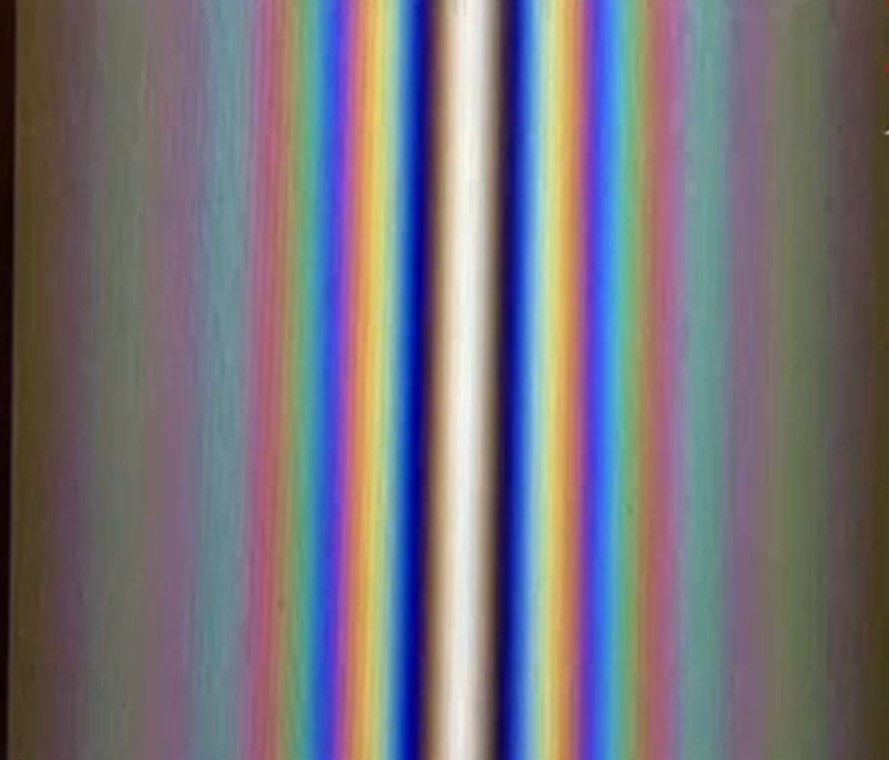
\includegraphics[width=\linewidth]{pic/spectreblanch.png}
                \end{minipage}
            \subsection{les Franges}
                \begin{minipage}{0.8\linewidth}
                    La distance entre deux FB ou deux FS est l'interfrange \boxed{i=\frac{\lambda D}{a}} \\
                    La distance entre FB et un FS est \boxed{\frac{i}{2}=\frac{\lambda D}{2a}} \\
                    comme dans lequation les position des franges depende de $\lambda $ sauf au centre 
                \end{minipage}
                \begin{minipage}{0.2\linewidth}
                    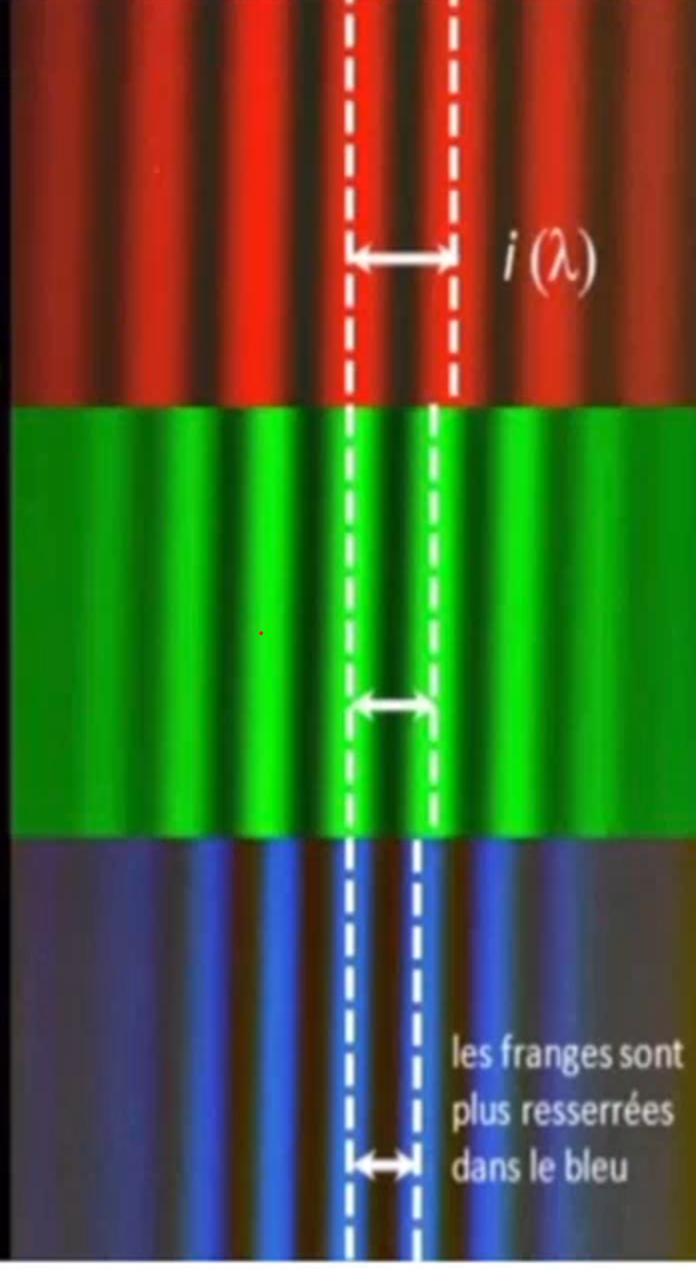
\includegraphics[width=\linewidth]{pic/frangepos.png}
                \end{minipage}
            \subsection{Position et grandeur de source}
                \begin{minipage}{0.6\linewidth}
                   Si la source est translatee lateralement , les franges d'interferences sont translatee on sense oppose
                \end{minipage}
                \begin{minipage}{0.4\linewidth}
                    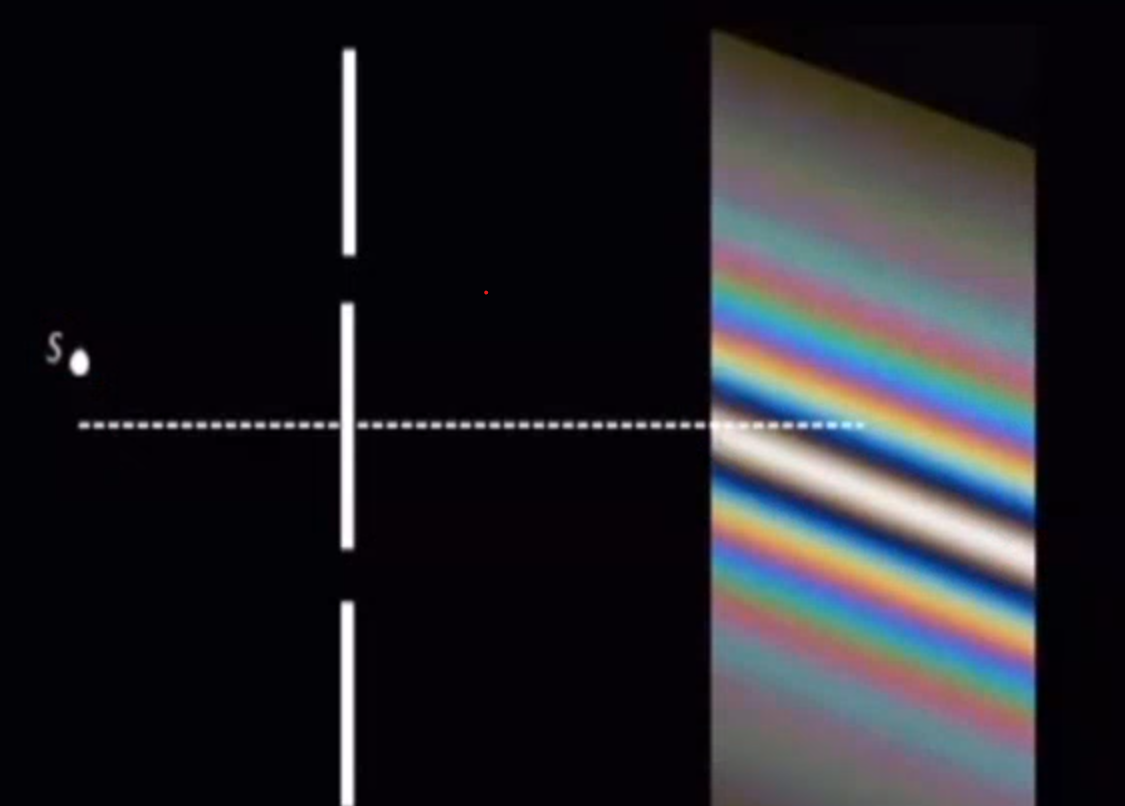
\includegraphics[width=\linewidth]{pic/sposition.png}
                \end{minipage} 
                \pagebreak
                Un bon contraste necessite une source peu etendue lateralement \\
                    \begin{minipage}{0.45\linewidth}
                        Large source\\
                        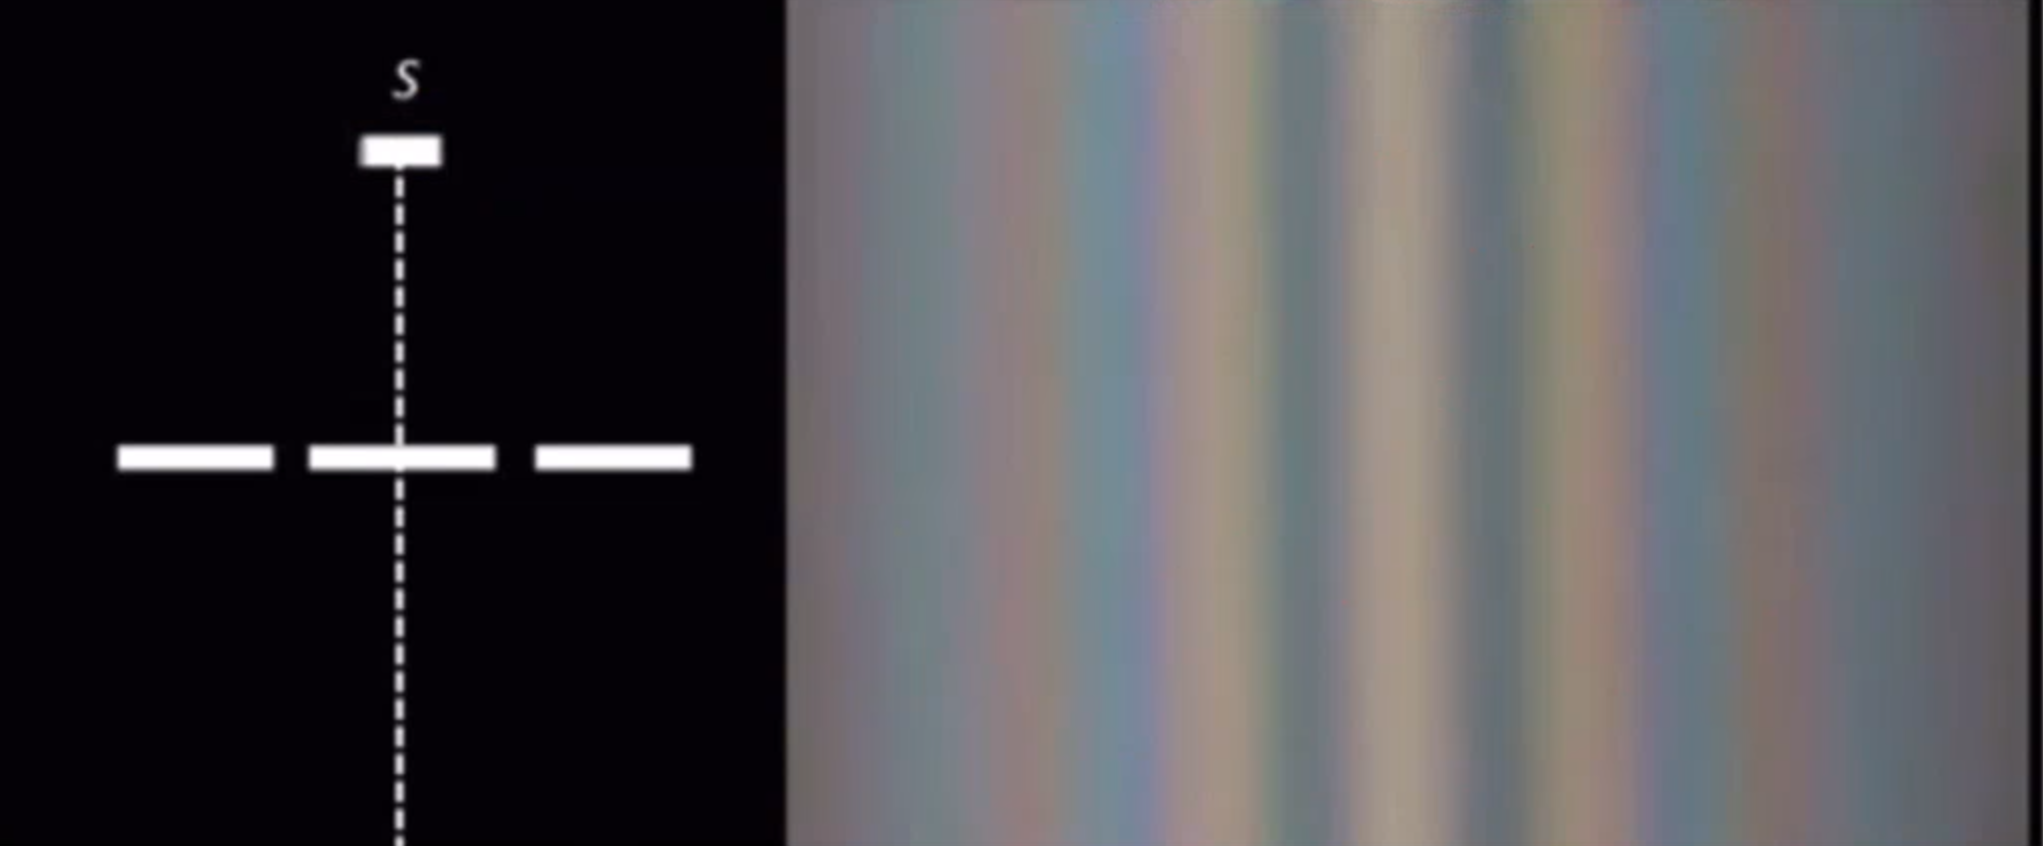
\includegraphics[width=\linewidth]{pic/ssize1.png}
                    \end{minipage}
                    \begin{minipage}{0.54\linewidth}
                        small source\\
                        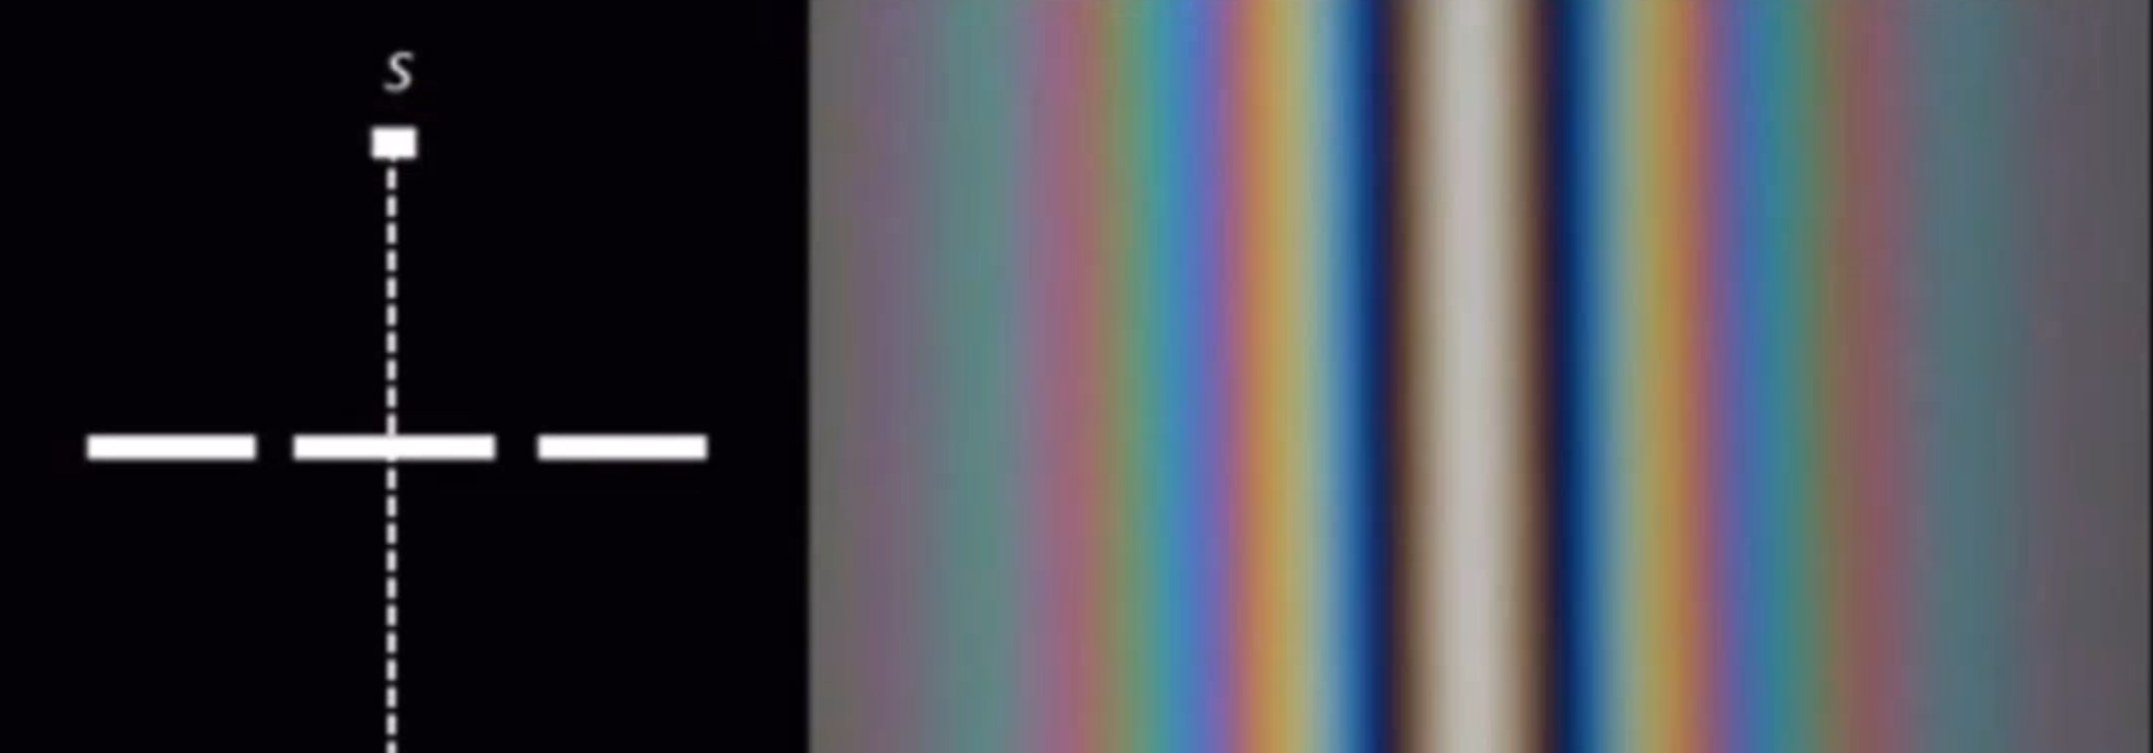
\includegraphics[width=\linewidth]{pic/ssize2.png}
                    \end{minipage}
            \subsection{Forme des franges d 'interference du dispositif d'Young}
                \begin{itemize}
                    \item les franges d'interference sont alors observees a l'endroit ou $\phi$ et $\delta$ sont constant 
                    \item 
                        \begin{minipage}{0.49\linewidth}
                            l endroit ou $\delta=r_2-r_1=cte$ definie une famille d'hyperboloides de revolution d'axe $S_1 S_2$ , Selon la direction d'observation et la taille du champ d'observation ,
                        les  franges pourront etre quasi-rectilignes, circularit \ldots
                        \end{minipage}
                        \begin{minipage}{0.49\linewidth}
                            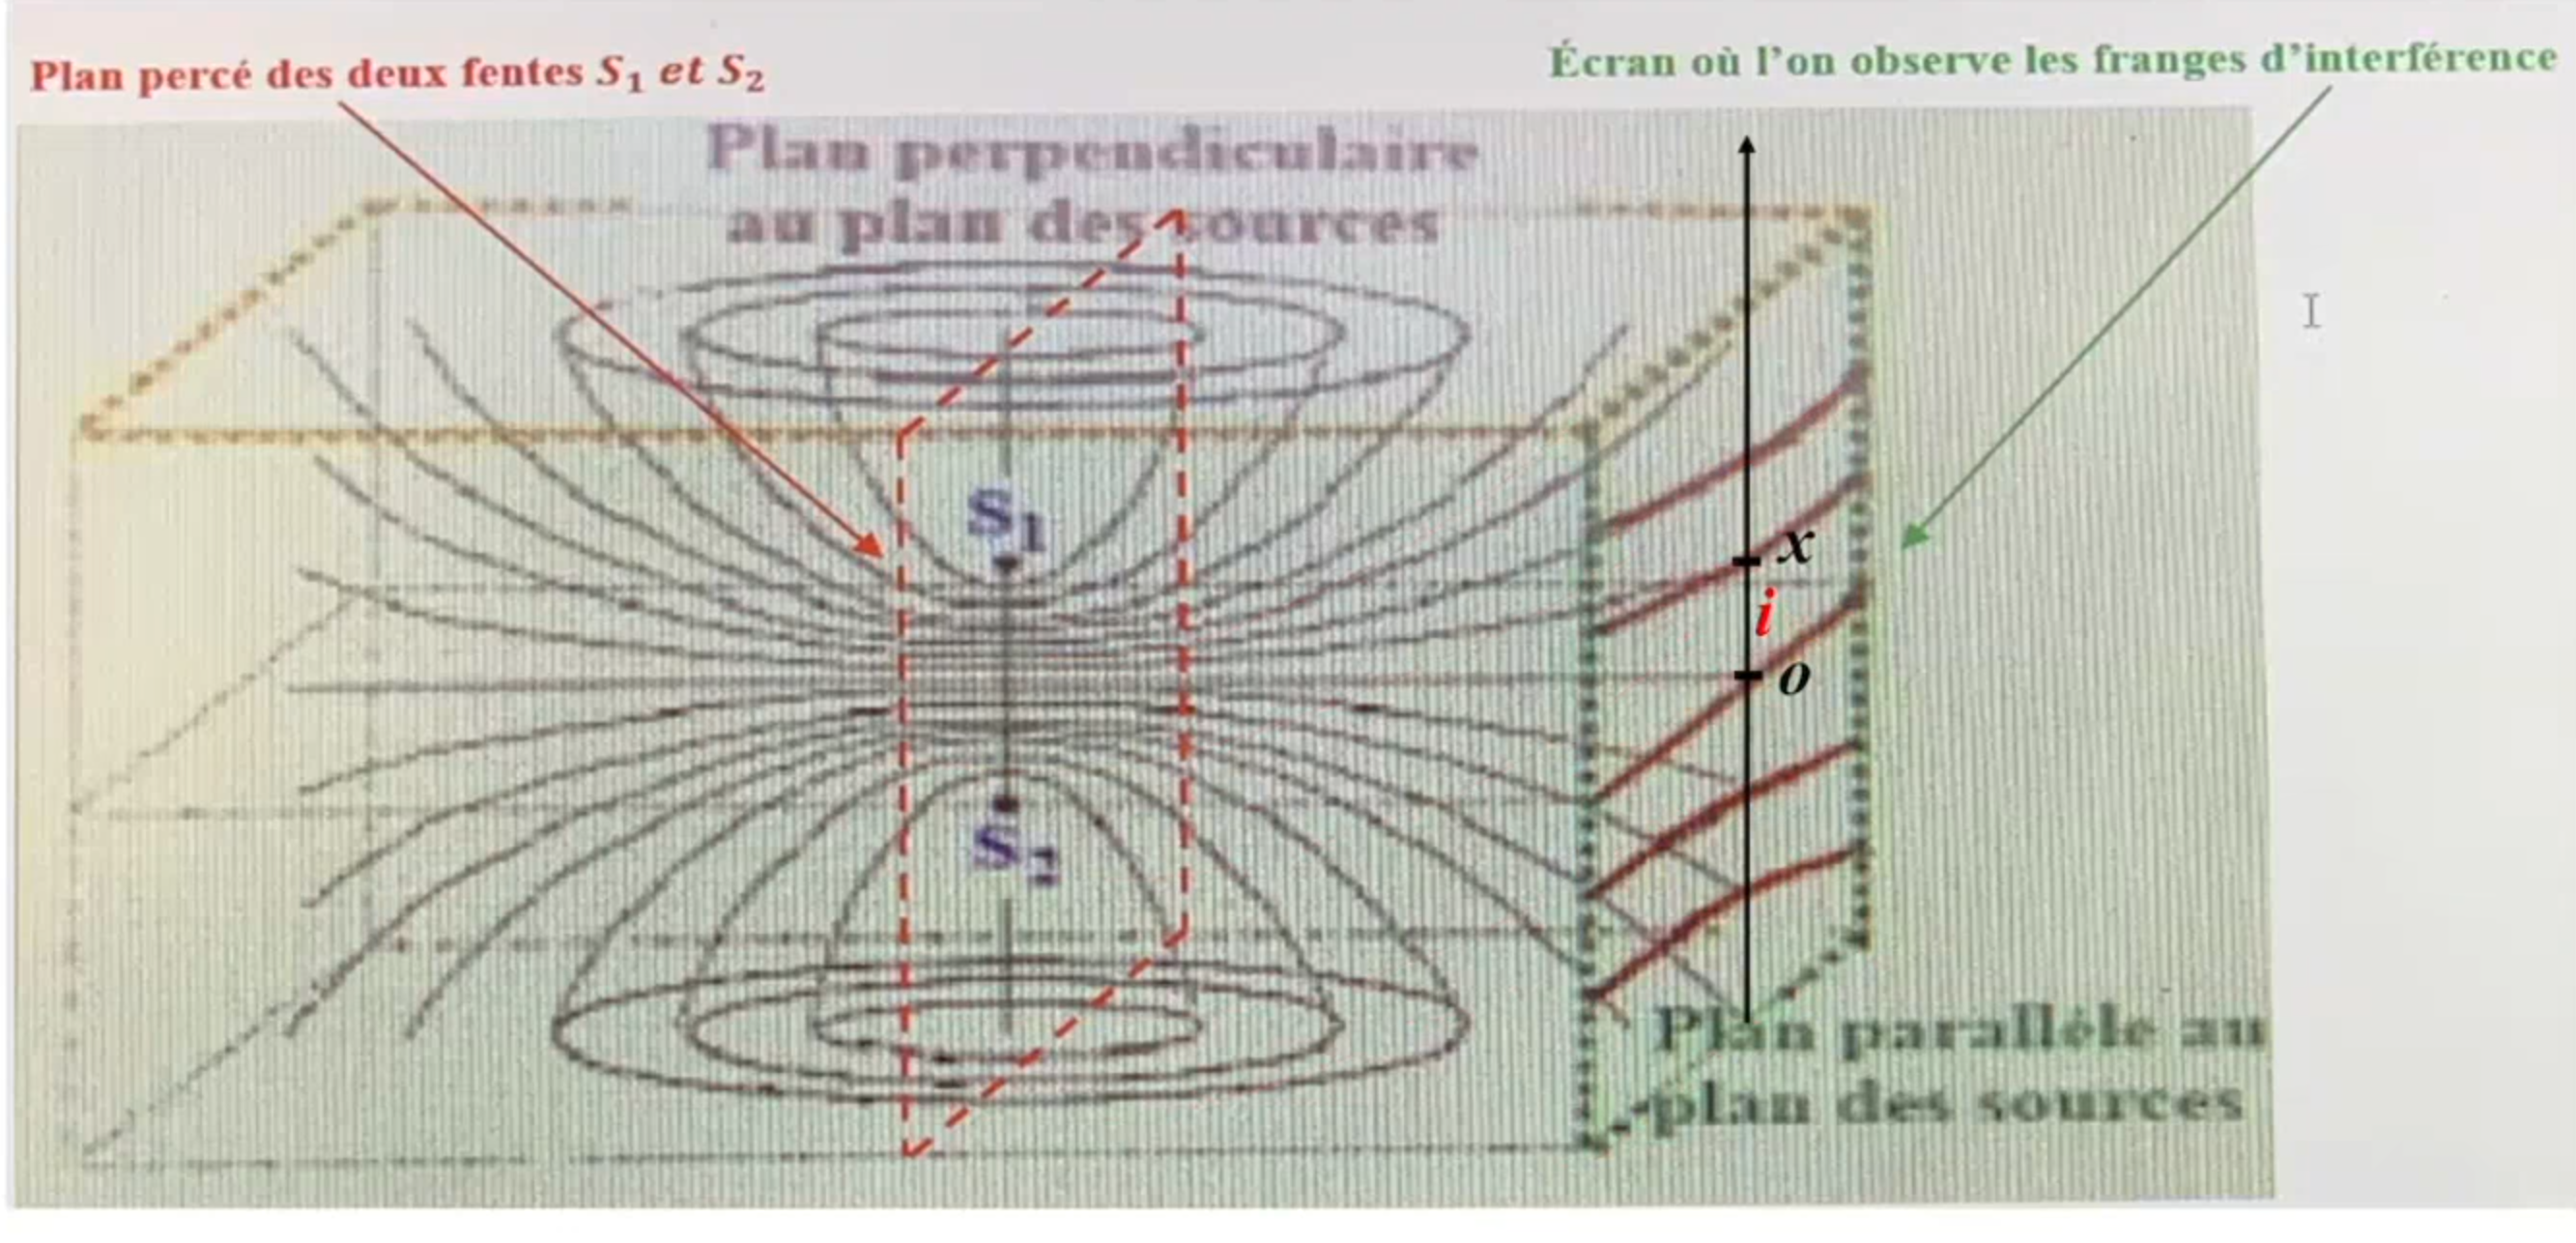
\includegraphics[width=\linewidth]{pic/hyperyoung1.png}
                        \end{minipage}
                    \item le dispositif d'young est donc interferometre a \underline{franges non localisee} , car en principe , on peut observer les franges d'nterference a n'import quel endroit du champ d'interference
                \end{itemize}
                \pagebreak
        \section{Pellicule mince}
            
            \begin{center}
                \begin{minipage}{0.59\linewidth}
                    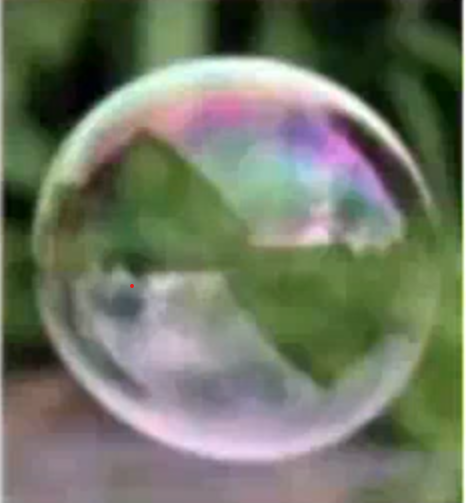
\includegraphics[width=0.2\linewidth]{pic/buble.png}
                    Un pellicule mince est une membrane transparente de faible epaisseur e et d'indic $n_p$ \\
                    Si on considere un angle d'incidence quasi normal , donc puisque $e$ est faible alors les s rayon 1 et 2 sont quasi-confondus\\
                    il s'agei d'une \underline{interference a division d'amplitude} . \\
                    On s'interesse donc au phenomene d'interference entre ces deux rayons 1 et 2 \vspace*{15px}
                \end{minipage}
                \begin{minipage}{0.38\linewidth}
                    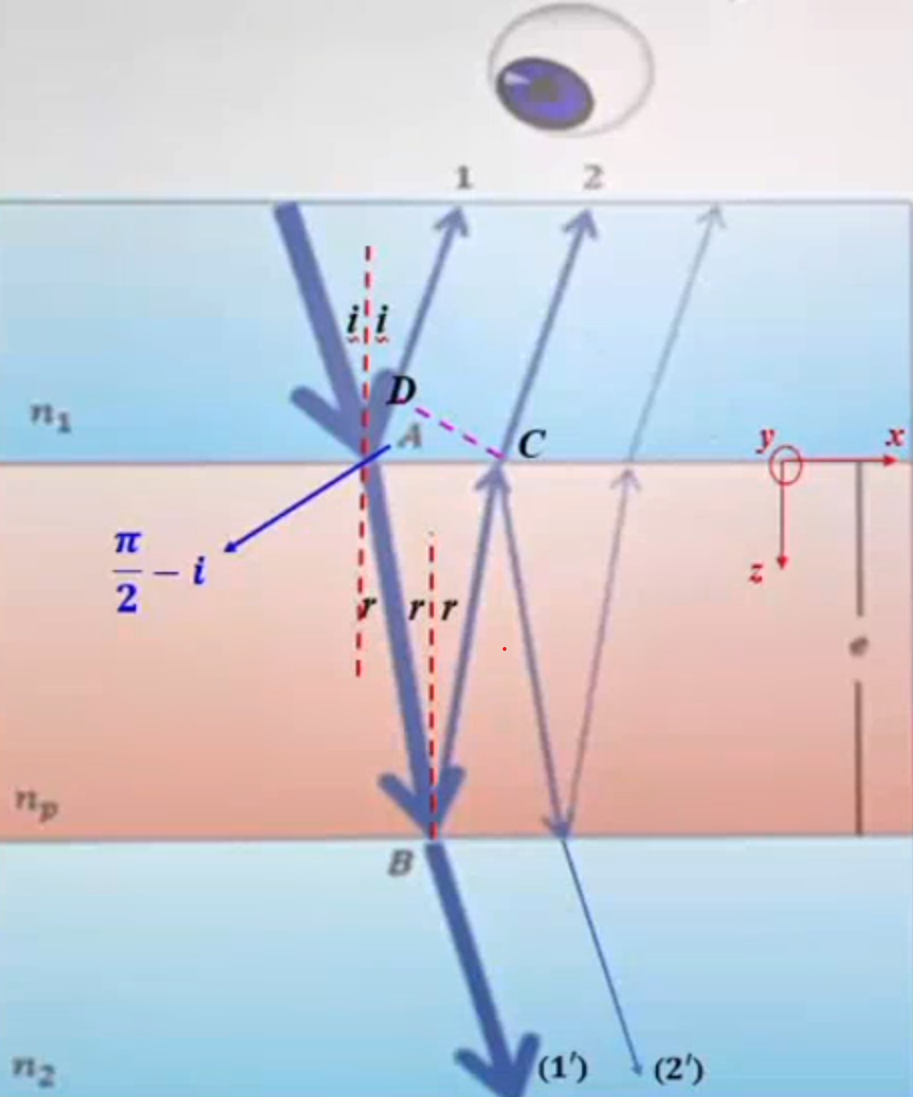
\includegraphics[width=\linewidth]{pic/pellicule.png}
                    
                \end{minipage}
            \end{center}
            \begin{itemize}
                \item  On a $\Delta\phi_{ps} = \frac{2\pi\delta}{\lambda}$
                \item Le rayon 1 dans le milieu 1 marche plus que le rayon 2 par une distance $ = AD \implies \underline{\delta_1^{'} = -n_1(AD)}$ \\
                    Le rayon 1 dans le milieu p march moins que le rayon 2 par une distance $= AB+BC\implies \underline{\delta_p^{'} = n_p(AB+BC)}$ \\
                    $\delta^{'} = n_p(AB+BC)-n_1AD \implies \underline{ \delta^{'}= 2n_pAB-n_1AD }$\\
                    $\underline{AB = \frac{e}{\cos(r)}}$ et $ AD=AC\cos(\frac{\pi}{2}-i)=AC\sin(i)=AC\frac{n_p}{n_1}\sin(r) $ avec $AC = 2e\tan(r) \implies AD =AC\frac{n_p}{n_1}\sin(r)\implies \underline{AD =\frac{2en_p\sin^2(r)}{n_1\cos(r)}}$ \\
                    $\delta^{'} =2n_pAB-n_1AD = 2n_p\frac{e}{\cos(r)} -n_1\frac{2en_p\sin^2(r)}{n_1\cos(r)} = \frac{2en_p\sin^2(r)}{n_1\cos(r)}(1-\sin^2(r))=\frac{2n_pe}{\cos(r)}\cos^2(r)$ \\
                    \begin{center}
                        \boxed{\delta^{'}=2n_pe\cos(r)}
                    \end{center}
                    \vspace*{15px}
                    il faut tenir compte d'un dephasage supplementaire du a la \underline{reflexion vitreuse} sur les deux faces de la lame ( en $A$ et $B $) 
                        $\begin{cases}
                            \text{Si } \phi_{\text{RV}} = 0 \text{ Alors la reflexion vitreuse est dite molle } \\
                            \text{Si } \phi_{\text{RV}} = \pi \text{ Alors la reflexion vitreuse est dite dure } \\
                        \end{cases}$ 
                \item le dephasage du la reflexion vitreuse est :$\Delta\phi_{\text{RV}} = \phi_{\text{BRV}} -\phi_{\text{ARV}} = {\phi_{\text{B}}}^\pi_0 - {\phi_{\text{A}}}^\pi_0$ \\
                    En supposant , pour simplifier , que la pellicule mince est placee dan l'air alors $n_1=n_2=1$ et donc$n_p > 1$ alors la reflexion vitreuse est \underline{externe} en $A$ et \underline{interne} en $B$\\
                    \begin{center}
                        \begin{minipage}{0.3\linewidth}
                            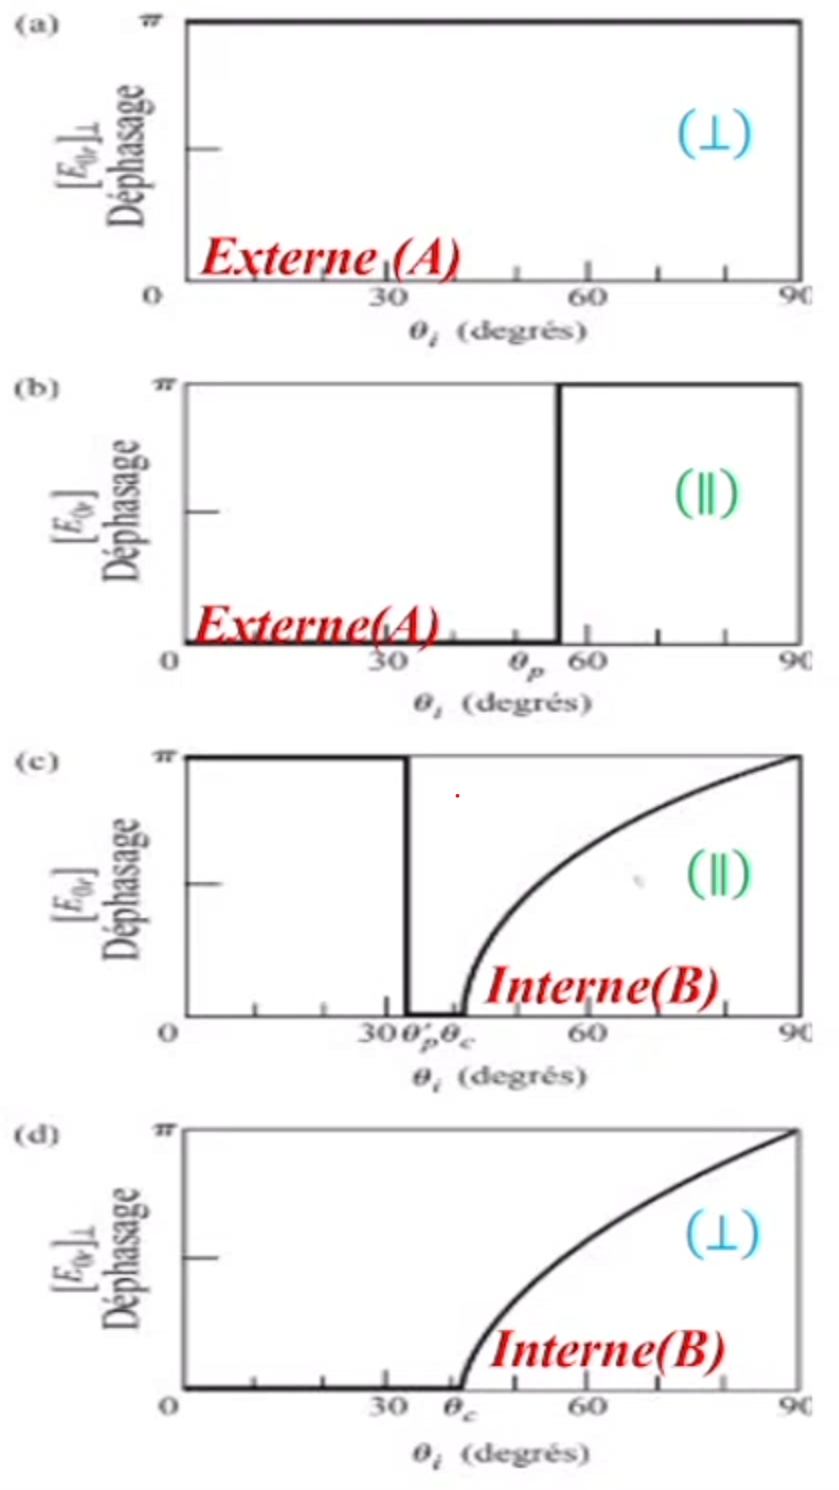
\includegraphics[width=\linewidth]{pic/reflexionvitreuses.png}
                        \end{minipage}
                        \begin{minipage}{0.69\linewidth}
                            Puisque on considere un angle d'incidence quasi normal alors \\
                            $\begin{cases}
                                \text{Polarisation ($\perp$)} \implies & \phi_A=\pi , \phi_B = 0 \\
                                \text{Polarisation ($\parallel$)} \implies & \phi_A=0 , \phi_B = \pi \\
                            \end{cases}$\\
                            $\begin{cases}
                                \Delta\phi_{tot\perp}=\Delta\phi_{ps} + \Delta\phi_{RV\perp} =\frac{2\pi\delta}{\lambda}-\pi \\
                                \Delta\phi_{tot\parallel}=\Delta\phi_{ps} + \Delta\phi_{RV\parallel} =\frac{2\pi\delta}{\lambda}+\pi \\
                            \end{cases}$ \\
                            Alors \boxed{\Delta\phi_{tot} = \frac{2\pi\delta}{\lambda}\pm\pi} \\
                            ou un dephasage de $\pm\pi$ correspond a une difference de marche de $\frac{\lambda}{2}$  
                        \end{minipage}
                    \end{center}
                \item Les Reflexion vitreuse decalent notre systeme de frange d'interference
                    \begin{itemize}
                        \item Interference Constructive\\
                            $\Delta\phi_{tot}= 2m\pi$\\
                            En polarisatoin ($ \perp $) :   $\Delta\phi_{tot}=\frac{2\pi\delta}{\lambda}-\pi=2m\pi\implies\frac{2\pi\delta}{\lambda}=(2m+1)\pi$\\
                            $\implies$ \boxed{\delta=(2m+1)\frac{\lambda}{2}}$\implies$ La frange centrale n'est plus Brilliant\\
                            En polarisatoin ($ \parallel $) :   $\Delta\phi_{tot}=\frac{2\pi\delta}{\lambda}+\pi=2m\pi\implies\frac{2\pi\delta}{\lambda}=(2m-1)\pi$\\
                            $\implies$ \boxed{\delta=(2m-1)\frac{\lambda}{2}}$\implies$ La frange centrale n'est plus Brilliant
                        \item Interference Destructive 
                            $\Delta\phi_{tot}= (2m+1)\pi$\\
                            En polarisatoin ($ \perp $) :   $\Delta\phi_{tot}=\frac{2\pi\delta}{\lambda}-\pi=(2m+1)\pi  \\ \implies\frac{2\pi\delta}{\lambda}=\pi + \pi + 2m\pi = 2m\pi$\\
                            $\implies$ \boxed{\delta=m\lambda}$\implies$ La frange centrale est sombre\\
                            En polarisatoin ($ \parallel $) :   $\Delta\phi_{tot}=\frac{2\pi\delta}{\lambda}+\pi=(2m+1)\pi \\ \implies\frac{2\pi\delta}{\lambda}=(2m-1)\pi-\pi=2m\pi$ \\ 
                            $\implies$ \boxed{\delta=m\lambda}$\implies$ La frange centrale est sombre\\
                    \end{itemize}
            \end{itemize}
        \section{Anneau de Newton}
            \begin{center}
                \begin{minipage}{0.69\linewidth}
                    \begin{itemize}
                        \item On eclaire sous incidence quasi-normale cette lentille de grand rayon R ,situee a une hauteur h au-dessus d'une lame plane 
                        \item Une partie du rayon incident (noir) se reflechit sur l'interface verre-air(rayon rouge) sans dephasage (reflexion interne en pol $\perp$)
                        \item L'autre partie du rayon incident (noir) traverse cette interface et se reflechit sur la lame inferieur (rayon blue) avex un dephasage de $\pi$ ( reflexion externe en pol $\perp$)
                        \item Comme on fait l'interference entre le rouge et le bleu , le rouge etant plus intense qui le bleu , alors cet interference reflete plus la symetrie circulair de la face circulaire de la lentille 
                        \item Les deux rayons reflechi (1) et (2) ( rouge t bleu )sont quasi-confondus et interferent en donnant des franges localisees au voisinge de la lentille 
                        \item les reflexion vitreuses decalent les franges $\implies$ la frange centrale est sombre
                    \end{itemize}
                \end{minipage}
                \begin{minipage}{0.3\linewidth}
                    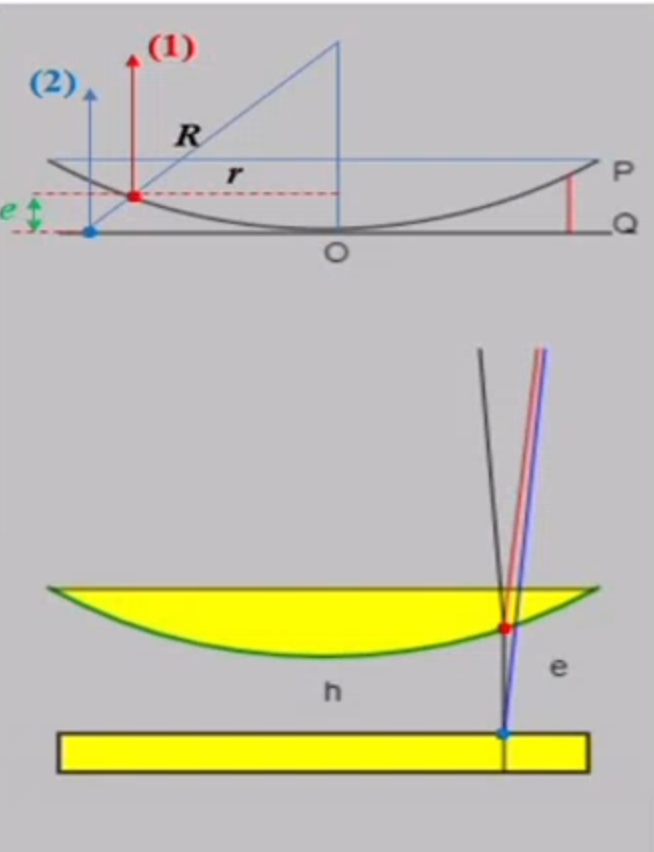
\includegraphics[width=\linewidth]{pic/newtonring1.png}
                    \\
                    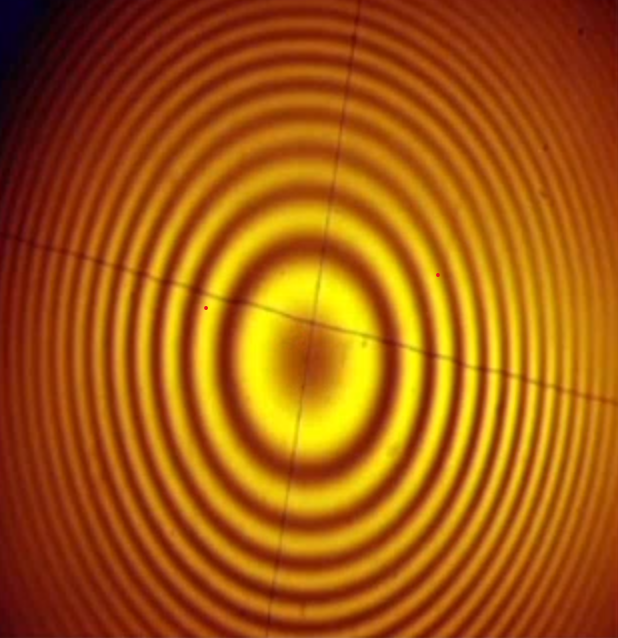
\includegraphics[width=\linewidth]{pic/newtonring2.png}
                \end{minipage}
            \end{center}
            Si $h=0$ alors la lentille est collee a la lame , et le coin d'air ainsi forme a pour epaisseur $e$ l'on cherche a determiner :\\
            $R^2= r^2+(R-e)^2 \implies R^2 - r^2 = (R-e)^2 \implies R-e = \sqrt{R^2-r^2} = (R^2-r^2)^{\frac{1}{2}}\implies e = R-(R^2-r^2)^{\frac{1}{2}} = R-R(1-\frac{r^2}{R^2})^{\frac{1}{2}}\approx R-R(1-\frac{1}{2}\frac{r^2}{R^2}) = \frac{1}{2}\frac{r^2}{R}$\\
            \boxed{\delta = 2e} \\
            Si $h \not = 0$ alors la lentille n'est plus collee a la lame , et le coin d'air ainsi forme a pour un epaisseur $e+h \implies $ \boxed{\delta = 2e +2h }


            Yep helloOh it's a nice feature to seeOK OKWanna watch in the summerone my heartbeat downhe used to be a friendwith the same gunno again don't don't use thatOK thank you thank you
        \section{Interferences a ondes multiples }    
            \begin{center}
                \begin{minipage}{0.7\linewidth}
                    \begin{itemize}
                        \item Les faces de cette lame sont legerment argentees pour augmenter les coefficient de reflexion 
                        \item L'onde incident principale va se reflechir un certain nombre de fois a l;interieur de cette lame avant de sortir des deux cotes de la lame 
                        \item On va etudier l;interference  par reflexion sur la 1er face de la lame et par transmission a travers la 2eme face de la lame
                    \end{itemize}
                \end{minipage}
                \begin{minipage}{0.29\linewidth}
                    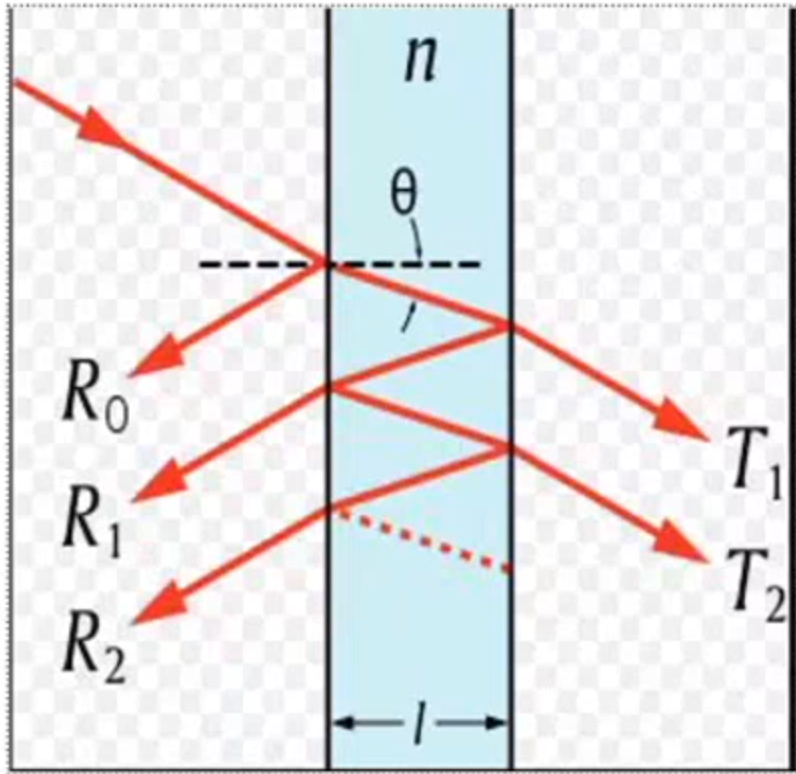
\includegraphics[width=\linewidth]{pic/interferencesaondesmultiples.png}
                \end{minipage}
            \end{center}
            \begin{center}
                \begin{minipage}{0.54\linewidth}
                    \begin{itemize}
                        \item La lame(substrat) est transparente d'indice $n$, d'epaisseur $d$ 
                        \item La lame est palce dans l'air
                        \item $r$ et $t$ les coefficient de reflexion et de transmission sur la face d'entree
                        \item $r^{'}$ et $t^{'}$ les coefficient de reflexion et de transmission sur la face d'sortie
                    \end{itemize}
                \end{minipage}
                \begin{minipage}{0.45\linewidth}
                    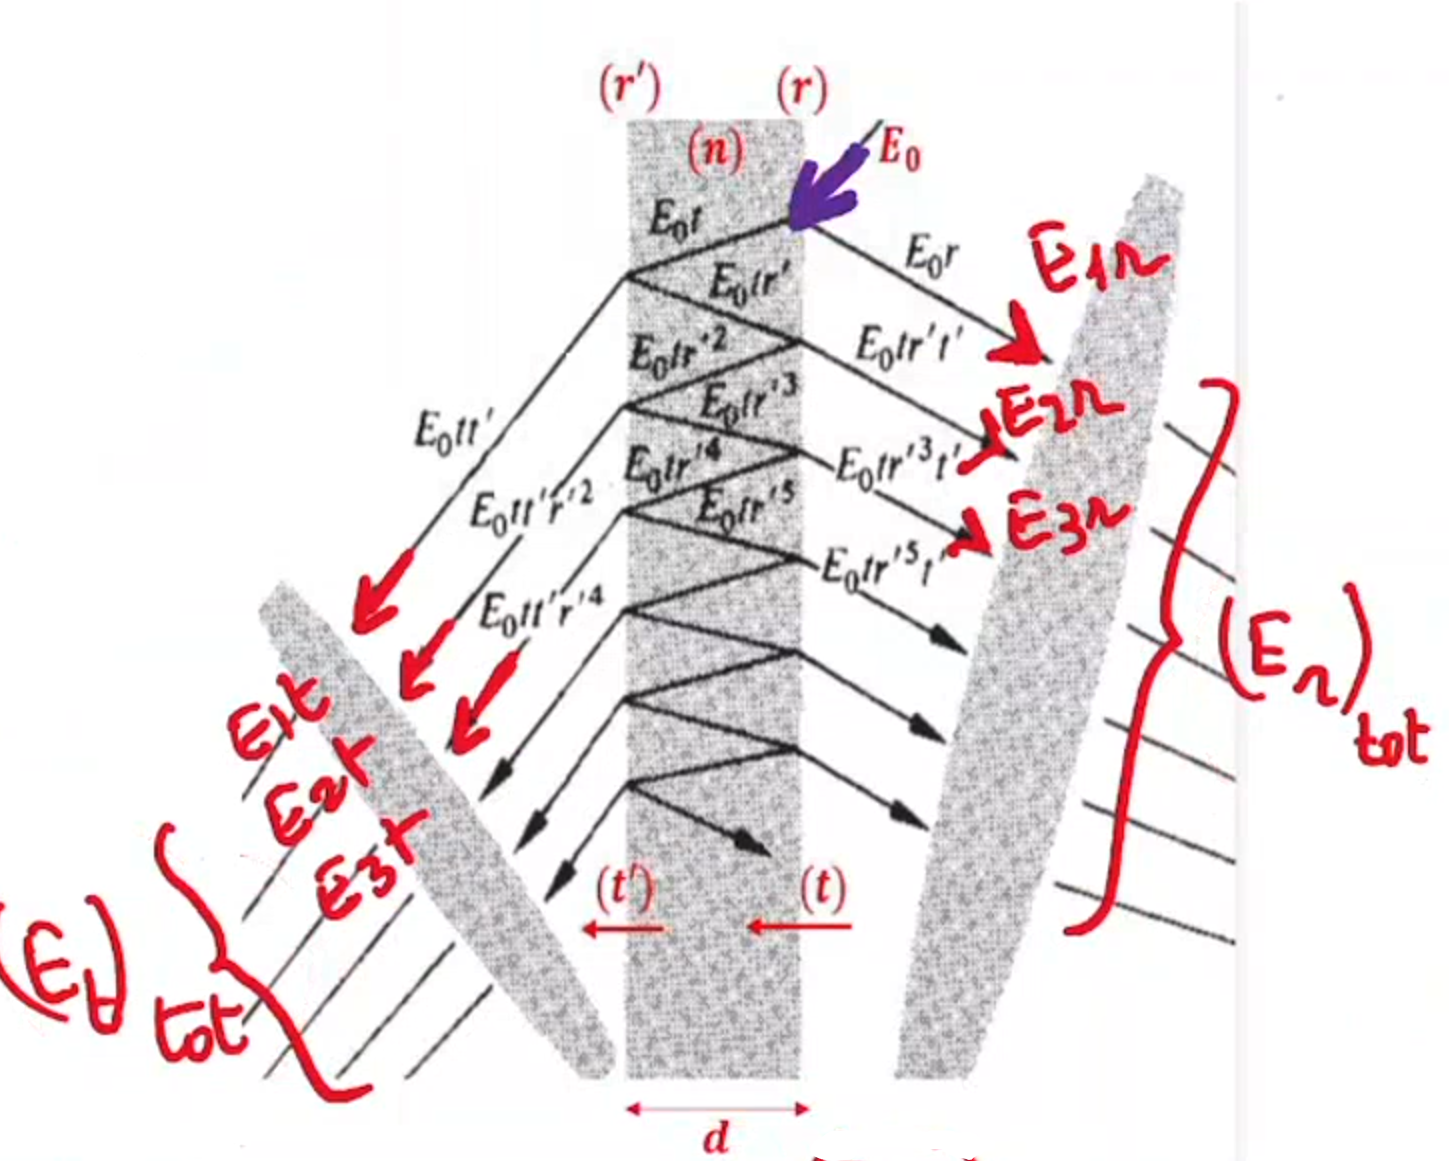
\includegraphics[width=\linewidth]{pic/lameinair.png}
                \end{minipage}
            \end{center}
            \begin{center}
                \begin{minipage}{0.64\linewidth}
                    Cette couche mince en peut la modulise par un matrice \\
                    \boxed{m_{ij} =
                        \begin{pmatrix}
                            m_{11} & m_{12} \\
                            m_{21} & m_{22}
                        \end{pmatrix} =
                        \begin{pmatrix}
                            \cos(kh) & \frac{i\sin(kh)}{Y_1} \\
                            i\sin(kh)Y_1 & \cos(kh) 
                        \end{pmatrix} 
                    }\\
                    Avec \begin{itemize}
                        \item $ k=\frac{2\pi}{\lambda} \text{ et } h = \frac{\delta}{2}$\\
                        \item $\begin{cases}
                            \text{polarisation $\perp$} & Y_1 = Y_{1\perp}=\frac{n_1}{120\pi}\cos(\theta_{i2})\\
                            \text{polarisation $\parallel$} & Y_1 = Y_{1\parallel}=\frac{n_1}{120\pi}\cos(\theta_{i2})
                            \end{cases}$
                        \item $\delta = (2d\cos(\theta_{t1}))=(2d\cos(\theta_{i2}))$
                    \end{itemize}
                    
                \end{minipage}
                \begin{minipage}{0.35\linewidth}
                    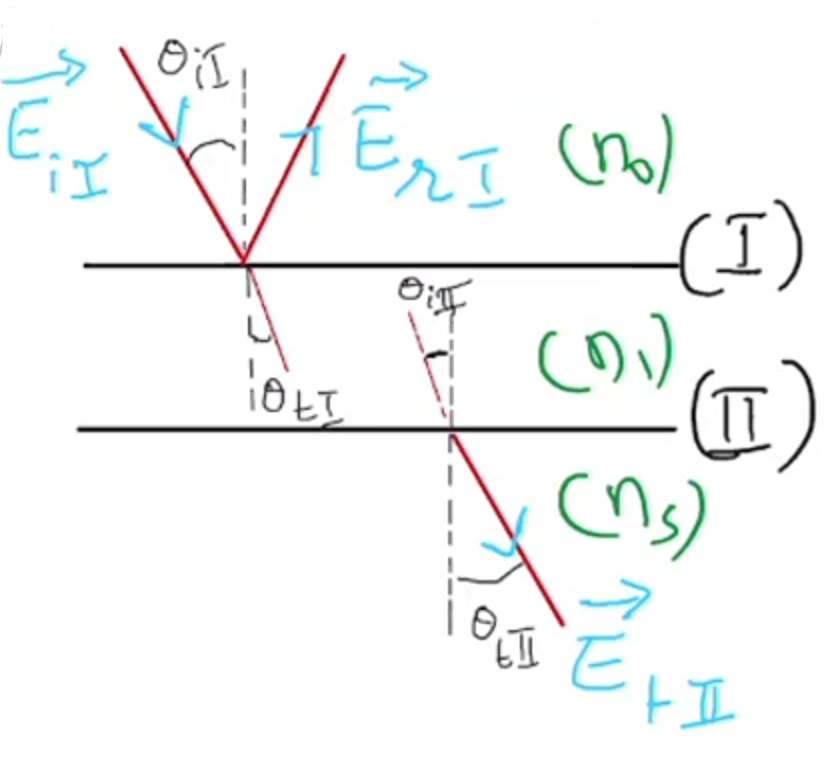
\includegraphics[width=\linewidth]{pic/lameinair2.png}\\
                    \begin{center}
                        $\begin{cases}
                            E_{i1} = E_0 \\
                            E_{r1}=(E_r)_{tot} \\
                            E_{t2}=(E_t)_{tot}
                        \end{cases}$
                    \end{center}
                \end{minipage} 
            \end{center}
            \pagebreak
            \underline{Coefficient de reflexion et de transmission} \\
            \begin{center}
                \boxed{r=\frac{E_{r1}}{E_{i1}} = \frac{Y_0m_{11}+Y_0Y_sm_{12}-m_{21}-Y_sm_{22}}{Y_0m_{11}+Y_0Y_sm_{12}+m_{21}+Y_sm_{22}}} \vspace*{20px}
                \boxed{t=\frac{E_{t2}}{E_{i1}} = \frac{2Y_0}{Y_0m_{11}+Y_0Y_sm_{12}+m_{12}+Y_sm_{22}}} \\
                \begin{minipage}{0.3\linewidth}
                    $\begin{cases}
                        Y_0 = \frac{n_0}{120\pi}\cos(\theta_{i1}) \\
                        Y_s = \frac{n_s}{120\pi}\cos(\theta_{i2}) \\
                    \end{cases}$
                \end{minipage}
                \begin{minipage}{0.2\linewidth}
                    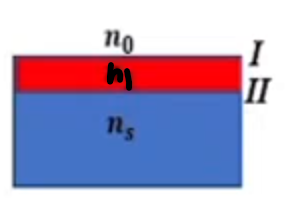
\includegraphics[width=\linewidth]{pic/lametopofshit.png}\\

                \end{minipage}
                \begin{minipage}{0.29\linewidth}
                    La lame est on rouge. \\
                    La lame est pose sur la substrat en blue.
                \end{minipage}
            \end{center}
            \subsection{Revetement antireflet a une couche quart d'onde}
                Anti reflet $\implies$ On cherche a anuller la reflexion  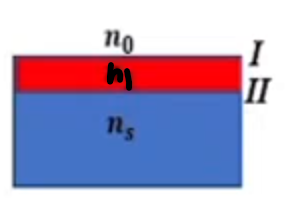
\includegraphics[width=0.3\linewidth]{pic/lametopofshit.png}\\
                A une couche quart d'onde $\implies$ On a metre une lame de face parallel d'epaisseur $d=\frac{\lambda}{4}$ sur le substrat et ona $h=\frac{\delta}{2}=d=\frac{\lambda}{4} \implies kh=\frac{2\pi}{\lambda}\frac{\lambda}{4}=\frac{\pi}{2} \\ \implies$\boxed{\cos(kh)=0} et \boxed{\sin(kh)=1}  \\
                $m_{ij} =
                \begin{pmatrix}
                    \cos(kh) & \frac{i\sin(kh)}{Y_1} \\
                    i\sin(kh)Y_1 & \cos(kh) 
                \end{pmatrix} =
                \begin{pmatrix}
                    0 & \frac{i}{Y_1} \\
                    iY_1 & 0
                \end{pmatrix} =
                \begin{pmatrix}
                    0 & \frac{i120\pi}{n_1} \\
                    \frac{in_1}{120\pi} & 0
                \end{pmatrix}$ \\
                et On a $r=\frac{E_{r1}}{E_{i1}} = \frac{Y_0m_{11}+Y_0Y_sm_{12}-m_{21}-Y_sm_{22}}{Y_0m_{11}+Y_0Y_sm_{12}+m_{21}+Y_sm_{22}} $ avec $\begin{cases} Y_0 = \frac{n_0}{120\pi} \\ Y_s = \frac{n_s}{120\pi}\end{cases} $ \\ 
                alors  $r = \frac{Y_0Y_sm_{12}-m_{21}}{Y_0Y_sm{12}+m_{21}} =\ldots = $\boxed{\frac{\frac{n_0n_s}{n_1}-n_1}{\frac{n_0n_s}{n_1}+n_1}}\\
                pour $r = 0 $ , $\frac{n_0n_s}{n_1}-n_1 = 0 \implies n_0n_s=n_1^2$\\
                Donc il faut fabrice un couche mince d epaisseur $\frac{\lambda}{4}$ et son indice $n=\sqrt{n_{a}n_{s}}$ avec $\begin{cases}
                    n_a \text{ est l indice de l air}\\
                    n_s \text{ est l indice de substrat}\\
                \end{cases}$
            \subsection{Revetement antireflet a double couche quart d'onde}
            Anti reflet $\implies$ On cherche a anuller la reflexion  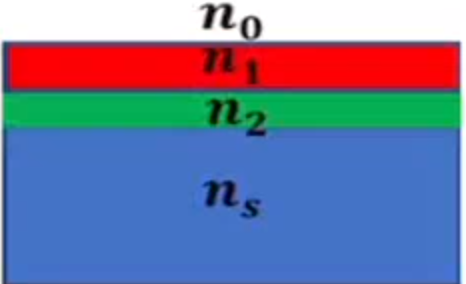
\includegraphics[width=0.3\linewidth]{pic/doublelametopofshit.png}\\
            A double couche quart d'onde $\implies$ On a metre deux lame de face parallel d'epaisseur $d_1=\frac{\lambda}{4}$ et $d_2=\frac{\lambda}{4}$ sur le substrat et ona   \\
            \begin{itemize}
                \item $h_1=\frac{\delta}{2}=d_1=\frac{\lambda}{4} \implies kh_1=\frac{2\pi}{\lambda}\frac{\lambda}{4}=\frac{\pi}{2} \implies$\boxed{\cos(kh_1)=0} et \boxed{\sin(kh_1)=1}
                \item $h_2=\frac{\delta}{2}=d_2=\frac{\lambda}{4} \implies kh_2=\frac{2\pi}{\lambda}\frac{\lambda}{4}=\frac{\pi}{2} \implies$\boxed{\cos(kh_2)=0} et \boxed{\sin(kh_2)=1}
            \end{itemize}
            Et On a : \\
            \begin{itemize}
                \item $M_1 =
                \begin{pmatrix}
                    \cos(kh_1) & \frac{i\sin(kh_1)}{Y_1} \\
                    i\sin(kh_1)Y_1 & \cos(kh)_1 
                \end{pmatrix} =
                \begin{pmatrix}
                    0 & \frac{i}{Y_1} \\
                    iY_1 & 0
                \end{pmatrix}$
                \item $M_2 =
                \begin{pmatrix}
                    \cos(kh_2) & \frac{i\sin(kh_2)}{Y_2} \\
                    i\sin(kh_2)Y_2 & \cos(kh)_2 
                \end{pmatrix} =
                \begin{pmatrix}
                    0 & \frac{i}{Y_2} \\
                    iY_2 & 0
                \end{pmatrix}$
                \item  $M = M_1 \times M_2 =\begin{pmatrix} 0 & \frac{i}{Y_2} \\ iY_2 & 0\end{pmatrix} \times\begin{pmatrix} 0 & \frac{i}{Y_1} \\iY_1 & 0 \end{pmatrix} = \begin{pmatrix} \frac{-Y_2}{Y_1} & 0 \\0 & \frac{-Y_1}{Y_2} \end{pmatrix} \implies$ \boxed{M =  \begin{pmatrix} \frac{-n_2}{n_1} & 0 \\0 & \frac{-n_1}{n_2} \end{pmatrix}} \\
                \item avec $Y_1 =\frac{n_1}{120\pi}$ , $Y_2 =\frac{n_2}{120\pi}$ , $Y_0 =\frac{n_0}{120\pi}$ , $Y_s =\frac{n_s}{120\pi}$
            \end{itemize}
            et On a $r=\frac{E_{r1}}{E_{i1}} = \frac{Y_0m_{11}+Y_0Y_sm_{12}-m_{21}-Y_sm_{22}}{Y_0m_{11}+Y_0Y_sm_{12}+m_{21}+Y_sm_{22}} =\ldots  \implies$\boxed{r=\frac{n_0n_2^2-n_1^2n_s}{n_0n_2^2+n_1^2n_s}} \\
            pour $r = 0 $ , $\frac{n_0n_2^2-n_1^2n_s}{n_0n_2^2+n_1^2n_s}\implies n_0n_2^2-n_1^2n_s =0$ \\
            Donc il faut satisfe l'equation suivant \boxed{\frac{n_2^2}{n_1^2}=\frac{n_s}{n_0}} en fabricent les deux couche mince 
            \pagebreak
    \chapter{Diffraction}
        \section{Phenomene de la diffraction}
            La diffraction est la deviation d'un faisceau de lumiere pres des bords d'un obstacle ou d'une overture \\
            tant que la taille de l'ouverture diffractante est $\approx \lambda$ , le phenomene de diffraction est observable 
            \begin{center}
                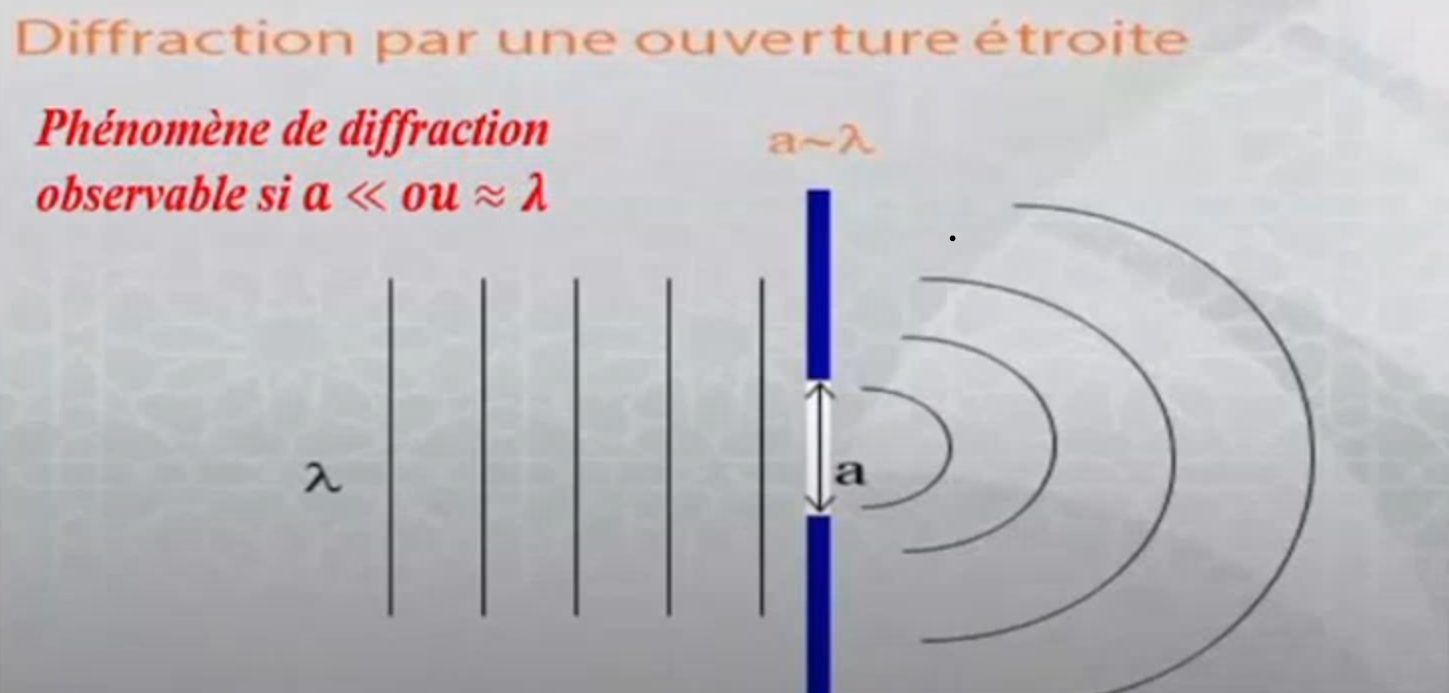
\includegraphics[width=0.4\linewidth]{pic/diffraction1.png}
                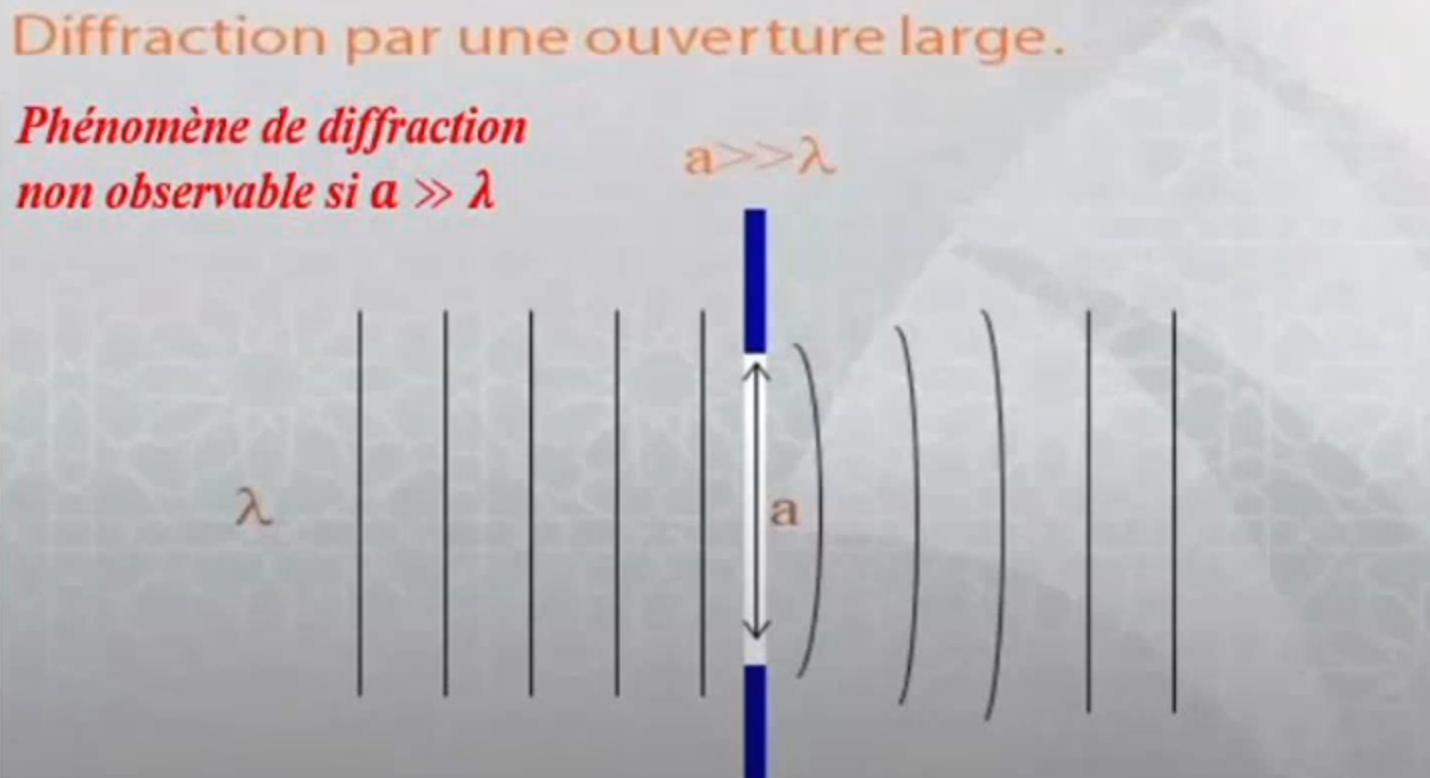
\includegraphics[width=0.4\linewidth]{pic/diffraction2.png}
            \end{center}
            Selon le principe de \underline{Huygens Fresnel} :
                \begin{itemize}
                    \item quand la source d'onde spherique eclaire une ouverture diffractante , alors chaque point de cette ouverture  est une source d'onde spherique secondaire 
                    \item Tant que la dimension de l'ouverture diffractante est $\approx \lambda $ toutes ces sources secondaires fictives sont coherentes entre elles  
                \end{itemize}
            Ces ondes spheriques secondaires vont interferer entre elles a des istances proches \underline{(diffraction de fresnel)} et a des  distances lointaines \underline{ (diffraction de Fraunhoger)} \\
            on a consacre a l'etude de la \underline{diffraction de fraunhofer}
        \section{Interference entre $N$ sources coherentes identiques a l'infine}
            \begin{minipage}{0.59\linewidth}
                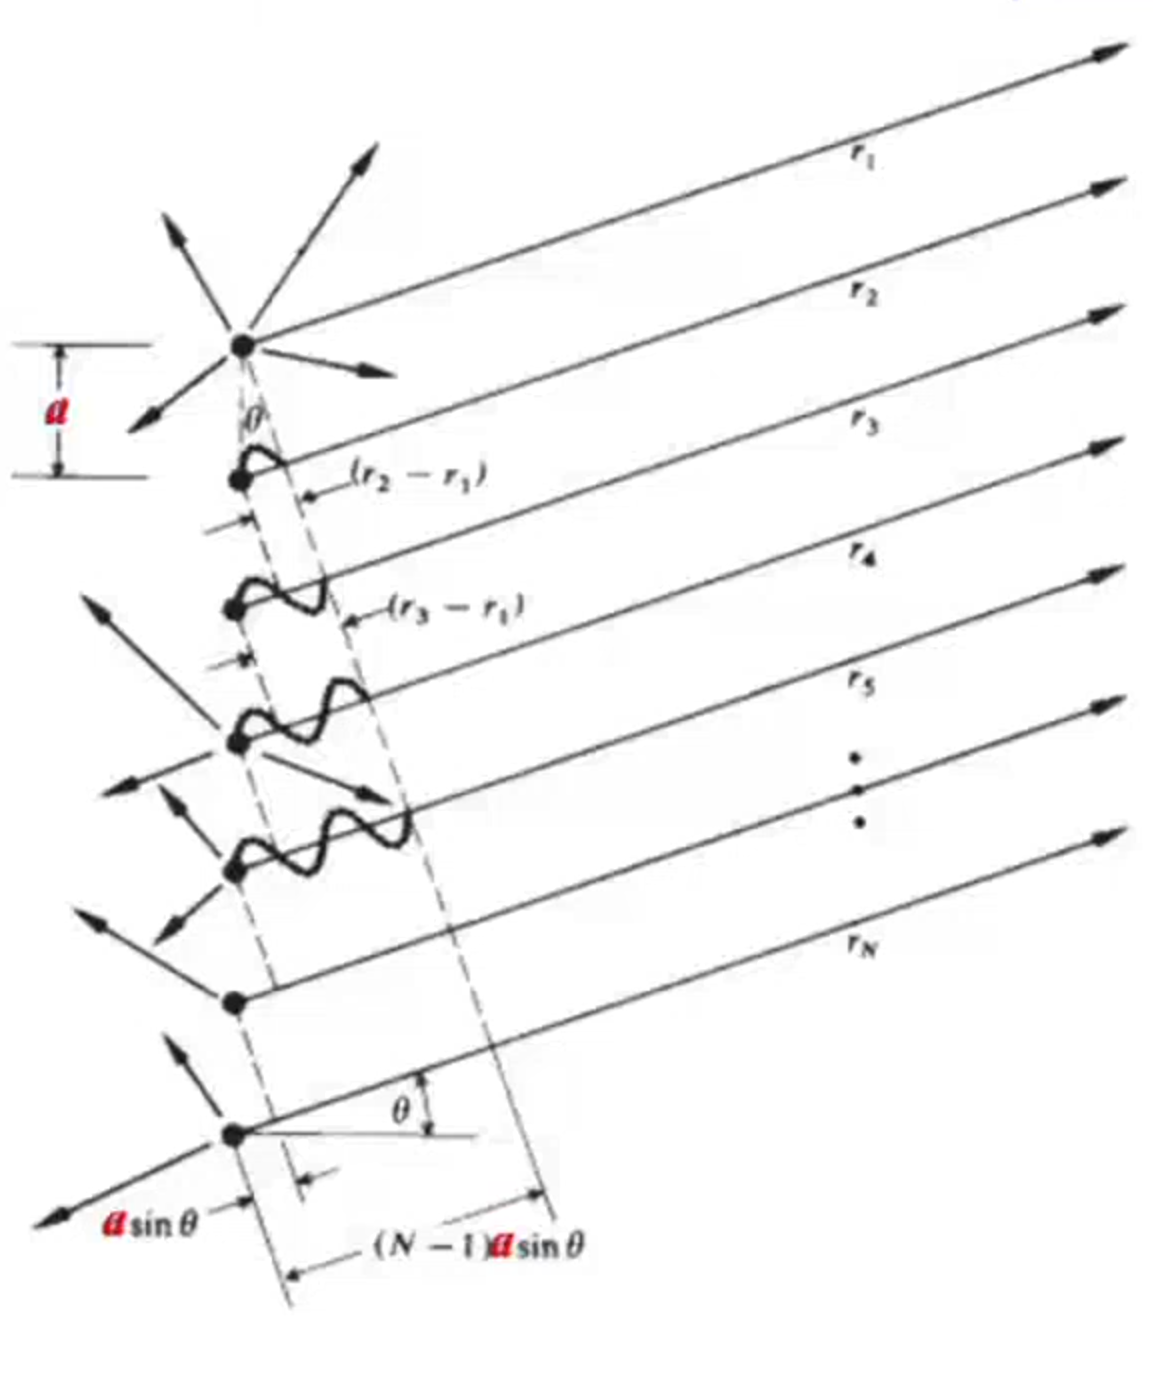
\includegraphics[width=\linewidth]{pic/diffraction3.png}
            \end{minipage}
            \begin{minipage}{0.39\linewidth}
                \begin{itemize}
                    \item Considerons une distribution discontinue de $N$ sources coherentes distantes de $a$ , $O$ est la centre de cette distribution 
                \end{itemize}
            \end{minipage}
            \begin{itemize}
                \item En point $P$ de l'ecran d'observation situe loin du plan de cette distribution , le champ resultant s' ecrit :\\
                        $E=E_0e^{i(kr_1-wt)}+E_0e^{i(kr_2-wt)}+\ldots+E_0e^{i(kr_N-wt)} $\\
                        $\implies E=E_0e^{i(kr_1-wt)}\left[1+e^{ik(r_2-r_1)}+e^{ik(r_3-r_1)}+\ldots+e^{ik(r_N-r_1)}\right] $\\ 
                        avec $\varphi$ est la difference de phase entre deux ondes successives distantes de a \\
                        $\varphi=\frac{2\pi\delta}{\lambda}=k\delta $ avec $\delta = r_2 - r_1 = a\sin(\theta) \approx \theta$(car $\theta$ est petit)\\
                        alors \boxed{E=E_0e^{i(kr_1-wt)}[1+e^{i\varphi}+e^{i2\varphi}+\ldots+e^{i(N-1)\varphi}]}
                \item On a donc une progression geometrique de raison $q=e^{i\varphi}$ et de premier terme $u_0 =1$ , la limite de cette progression est : \\
                    $[1+e^{i\varphi}+e^{i2\varphi}+\ldots+e^{i(N-1)\varphi}]=u_0\frac{1-q^N}{1-q} = \frac{e^{iN\varphi}-1}{e^{i\varphi} - 1} \implies E=E_0e^{i(kr_1-wt)}\frac{e^{iN\varphi}-1}{e^{i\varphi} - 1} $
                    $E_0e^{i(kr_1-wt)}\frac{e^{iN\varphi}-1}{e^{i\varphi} - 1} = E_0e^{i(kr_1-wt)}\frac{e^{i\frac{N\varphi}{2}}}{e^{i\frac{\varphi}{2}}}\left[ \frac{e^{iN\frac{\varphi}{2}} - e^{-iN\frac{\varphi}{2}}}{e^{i\frac{\varphi}{2}}- e^{-i\frac{\varphi}{2}}} \right] \implies $\boxed{E=E_0e^{i(kr_1+(N-1)\frac{\varphi}{2})}\left[ \frac{\sin(N\frac{\varphi}{2})}{\sin(\frac{\varphi}{2})} \right]} \\
                \pagebreak 
                \item Le dephasage entre la 1ere onde et la N ieme onde est : \\
                    $r_N-r_1=(N-1)a\sin(\theta)\implies r_N=r_1+(N-1)a\sin(\theta)$ \\
                    Si R est la distance entre le centre $O$ de cette distribution et le point $P$ de l'ecran $\implies$ en R on a la moitie du nombre de sources , soit $N/2$ ($R=r_{\frac{N}{2}}$)\\
                    $R = r_1 + \frac{1}{2}(N-1)a\sin(\theta)$ avec $\varphi = \frac{2\pi\delta}{\lambda}=k\lambda=ka\sin(\theta)\implies a\sin(\theta) = \frac{\varphi}{k} \implies R = r_1 + \frac{1}{2}(N-1)\frac{\varphi}{k} \implies $\boxed{kR = kr_1 + \frac{\varphi}{2}(N-1)} \\
                \item On a Le champ resultant en P s'ecrit : $E = E_0e^{-iwt}e^{i[kr_1+(N-1)\frac{\varphi}{2}]}\left[ \frac{\sin(N\frac{\varphi}{2})}{\sin(\frac{\varphi}{2})} \right]$ \\
                    alors \boxed{E=E_0e^{i(KR-wt)}\left[ \frac{\sin(N\frac{\varphi}{2})}{\sin(\frac{\varphi}{2})} \right]}
                \item L intensite lumineuse au point $P$ est $I \equiv \frac{1}{2}E.E^{*} \\ \implies $\boxed{I=I_0\frac{\sin^2(N\alpha)}{\sin^2(\alpha)}} avec $\alpha = \frac{\varphi}{2}=\frac{\pi a \sin(\theta)}{\lambda} $
                    \begin{center}
                        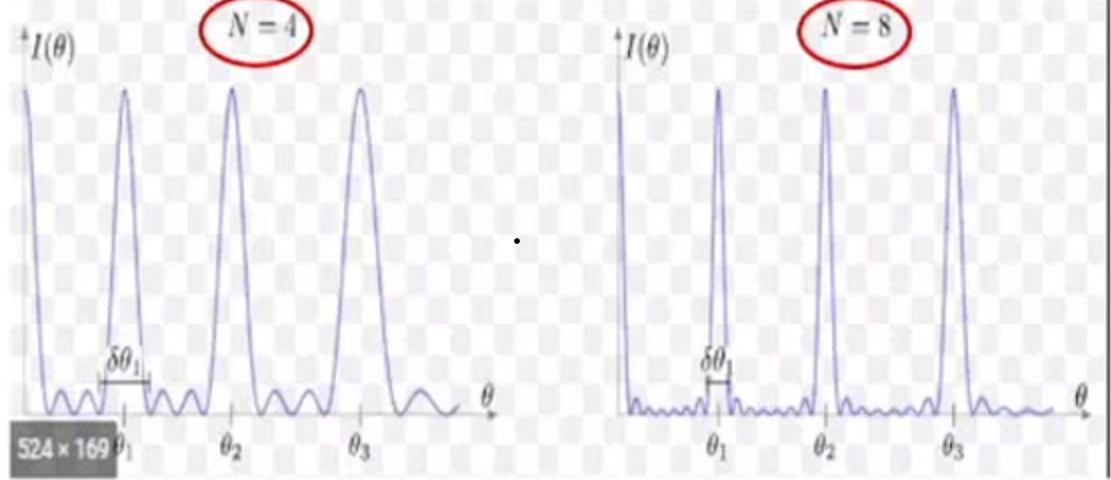
\includegraphics[width=0.5\linewidth]{pic/reseaudediffraction1}
                        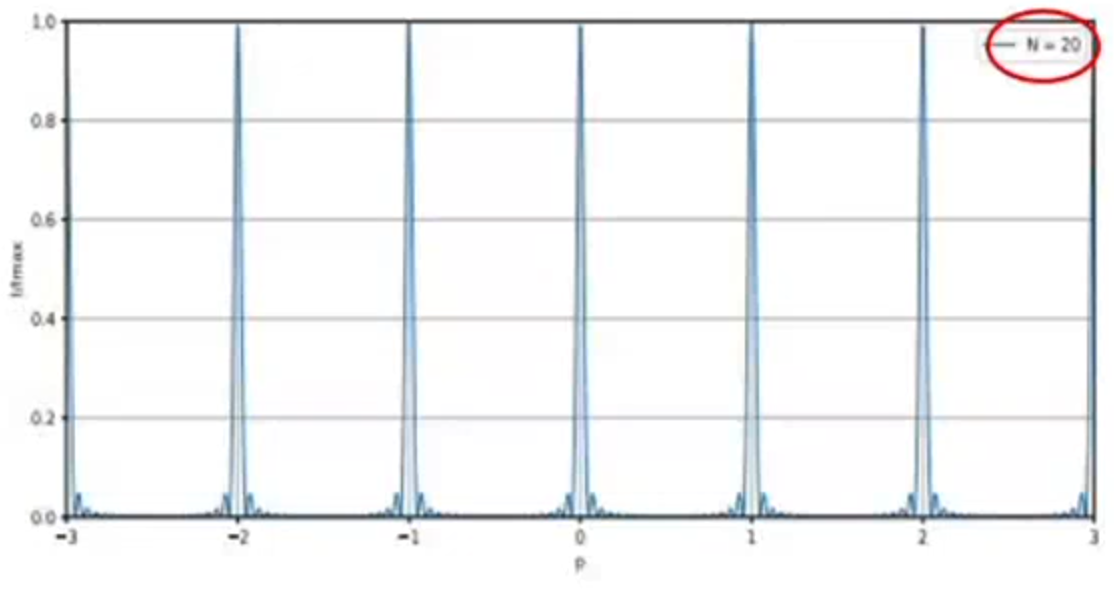
\includegraphics[width=0.49\linewidth]{pic/reseaudediffraction2}
                    \end{center}
                \item Les maximas Principaux de $I$ s'obtiennent pour :\\
                    $\varphi = 2m\pi=\alpha=m\pi\implies $\boxed{\delta = a\sin(\theta)=m\lambda}$ \implies \sin(\theta) \approx \theta =\frac{m\lambda}{a}=\frac{\lambda}{a}(m)$\\
                    Les minimas (les zeros )de $I$ s'obtiennent pour : \boxed{n\alpha=m\pi} (m est lordre d interference)
                \item Entre deux Maximas Principaux de $I$ il y a $(N-2)$ Maxiamas secondaires et $(N-1)$ minimas de $I$
                \item Les franges brillantes d'interference sont des raies extremement fines avec lesquelles on identifie l'ordre $m$ d'interference
                \item le pic central $(m=0) $et les autres pics sont d ordres $ m = \pm 1, \pm 2 ,\ldots$
                \item les zones sombres sont relativement larges 
                \item type des reseau de diffraction \\
                    \includegraphics[width=0.49\linewidth]{pic/reseaudediffractionpartransmission.png}
                    \includegraphics[width=0.49\linewidth]{pic/reseaudediffractionparreflexion.png}
                \item \begin{minipage}{0.49\linewidth}
                    dans le cas d incidente oblique \boxed{\delta = a\sin(\theta) - a\sin(\theta_i)} avec $\theta_i \not = 0$
                \end{minipage}
                \begin{minipage}{0.49\linewidth}
                    \includegraphics[width=0.49\linewidth ]{pic/reseaudediffractionoblique.png}
                \end{minipage}
                \item Dans une reseaux de diffraction on definit aussi la frequence $f$ du reseau par : le nombre de ligne par period (a) encm  : \boxed{f=\frac{1}{a}} 
                \item Pouvoir dispersif du reseau \boxed{D=\frac{\Delta\theta_m}{\Delta\lambda}} \\ c-a-d Si on eclaire le reseau par une lumiere polychromatique ($\lambda $ est variable) alors pour le meme $m$ on a differents $\Delta\theta_m$ avec$\theta_m$ est l angle d raies d'ordre $m$ 
            \end{itemize}
        \section{Diffraction de Fraunhofer}      
            \subsection{Diffraction de Fraunhofer a travers une fente de largeur a}
                On considere une fente de largeur $a \approx \lambda$ selon l'axe des $x$ et de longueur tres grande selon l'axe des y \\
                Chaque point de cette fente est une source secondaire d'onde \\
                Toutes ces ondes secondaires emises par la fente sont coherentes entre elles \\
                Ces ondes interferent sur l'ecran situe loin du plan de la fente
                \begin{center}
                    \includegraphics[width=0.7\linewidth]{pic/diffractionfente.png}
                \end{center}
                Il existe une distribution continue des sources sur la largeur $(a)$ de la fente , si la source principale eclaire la fente avec des rayons paralleles \\
                $\implies E = E_0e^{i(kr_1-wt)}\int^{+\frac{a}{s}}_{-\frac{a}{s}}e^{+i\varphi}dx $avec $\varphi = \frac{2\pi\delta}{\lambda}$ et $\delta = x\sin(\theta)\approx x\theta$  \\
                $\implies  E = E_0e^{i(kr_1-wt)}\int^{+\frac{a}{s}}_{-\frac{a}{s}}(\cos(\varphi)+i\sin(\varphi))dx = E_0e^{i(kr_1-wt)}\left[ \int^{+\frac{a}{s}}_{-\frac{a}{s}}\cos(\varphi)dx + i\int^{+\frac{a}{s}}_{-\frac{a}{s}}\sin(\varphi)dx \right]$\\
                $\varphi = \frac{2\pi x\theta}{\lambda}\implies i\int^{+\frac{a}{s}}_{-\frac{a}{s}}\sin(\varphi)dx =0$ \\
                $\implies E = E_0e^{i(kr_1-wt)}\int^{+\frac{a}{s}}_{-\frac{a}{s}}\cos(\varphi)dx \implies E =  E_0e^{i(kr_1-wt)} \frac{1}{\frac{2\pi\theta}{\lambda}}\left[ \sin(\frac{2\pi a \theta}{2\lambda}) -\sin(\frac{2\pi(-a)\theta}{2\lambda}) \right] $\\
                $\implies$ \boxed{E=aE_0e^{i(kr_1-wt)}\frac{\sin(\frac{\pi a \theta}{\lambda})}{\frac{\pi a \theta}{\lambda}}}\\
                Puisque l'intensite lumineuse est $I = \frac{1}{2}E.E^{*} \implies $
                \begin{center}  
                    \begin{minipage}{0.6\linewidth}
                        \boxed{I_{\text{diff}} = \frac{1}{2}a^2E_0^2\frac{(\sin(\frac{\pi a \theta }{\lambda}))^2}{(\frac{\pi a \theta}{\lambda})^2} = I_m\frac{(\sin(\beta))^2}{\beta^2}}\\
                        avec $\beta = \frac{\pi a \theta}{\lambda} \approx \frac{\pi a \sin(\theta)}{\lambda}=\frac{\varphi}{2}$ et $\theta = \sin(\theta)=\frac{X}{D}$
                    \end{minipage}
                    \begin{minipage}{0.39\linewidth}
                        \includegraphics[width=\linewidth]{pic/diffractionscheme.png}
                    \end{minipage}
                \end{center}
                Le Courbe de $I_{\text{diff}}$\\
                \begin{center}
                    \begin{minipage}{0.39\linewidth}
                        \includegraphics[width=\linewidth]{pic/diffractioncourbe.png}
                    \end{minipage}
                    \begin{minipage}{0.59\linewidth}
                        \includegraphics[width=\linewidth]{pic/diffractionimage1.png}
                    \end{minipage}
                \end{center}
                Les minimas (zeros) sont pour \boxed{\beta =m\pi} , $\frac{a\theta}{\lambda}=m $ avec \boxed{m \not = 0} , $X=m\frac{\lambda D}{a} \implies I_{min} = 0$ \\
                La maximal principal est pour  $m = 0 \implies \beta =0 \implies \sin(\beta ) = \beta \implies I_{\text{max principal}}$\\
                Les maximas secondaires sont pour \boxed{\beta = (2m+1)\frac{\pi}{2}} , $\frac{a\theta}{\lambda} = (m+\frac{1}{2})$  ,\\  $I_{\text{max secodaires}} = \frac{I_m}{(\pi(m+\frac{1}{2}))^2}$
            \subsection{Diffraction de Fraunhofer a travers une fente rectangulaire de dimension $a \times b$}    
                Dans le cas de fente rectangulaire il existe une distribution continue des sources sur la largeur (a) et la longuer (b) de la fente , si la source principale eclaire la fente avec des rayons paralleles \\
                \boxed{E = abE_0e^{i(kr_1-wt)}\frac{\sin(\frac{\pi a X}{\lambda D})\sin(\frac{\pi b Y}{\lambda D})}{\frac{\pi a X}{\lambda D } \frac{\pi b Y }{\lambda D}}  }\\
                l intensite lumineuse au point P n'est pas autre que $ I =\frac{1}{2}E.E^{*} \\ 
                \implies $ \boxed{\frac{1}{2}a^2b^2E_0^2\left(\frac{ \sin(\frac{\pi b Y}{\lambda D}) }{ \frac{\pi b Y }{\lambda D} }\right)^2\left(\frac{ \sin(\frac{\pi a X}{\lambda D}) }{ \frac{\pi a X }{\lambda D} }\right)^2 = I_m \frac{\left( \sin(\frac{\pi b Y}{\lambda D})\right)^2}{ \left(\frac{\pi b Y }{\lambda D} \right)^2}\frac{ \left(\sin(\frac{\pi a X}{\lambda D}) \right)^2}{ \left(\frac{\pi a X }{\lambda D}\right)^2 }} \\
                \begin{center}
                    \includegraphics[width=0.49\linewidth]{pic/diffractionfenterectangulair1.png}
                    \includegraphics[width=0.49\linewidth]{pic/diffractionfenterectangulair2.png}
                \end{center}
        \pagebreak
        \section{Interfernce a deux ondes modulees par la diffraction}
            Si on a deux fente identique de largeur $b \approx \lambda$, chacune et distantes de $a$ , alors on peut observer en meme temps :
            \begin{itemize}
                \item La diffraction a travers chaque fente de largeur $b$
                \item L'interference a travers ces deux fente distantes de $a$.
            \end{itemize}
            Le phenomen d'interfernece entre les deux fentes se fera entre ces deux intensite diffractees \\ 
           
            \begin{center}
                \begin{minipage}{0.5\linewidth}
                    \includegraphics[width=\linewidth]{pic/interferencediffraction.png}
                    \includegraphics[width=\linewidth]{pic/interferencediffractiondescription.png}
                \end{minipage}
                \begin{minipage}{0.49\linewidth}
                    $ I = 4I_0\cos^2(\frac{\varphi}{2})=4I_0\cos^2(\alpha) $\\
                    $\implies$\boxed{I =4\left[ I_m\left( \frac{\sin^2(\beta)}{\beta^2} \right) \right]\cos^2(\alpha)}\\
                    avec $\beta = \frac{\pi b \sin(\theta)}{\lambda}$ et $ \alpha = \frac{\pi a \sin(\theta)}{\lambda} $ 
                    \begin{itemize}
                        \item Maximum central de diffraction : $\beta = 0$
                        \item Minimas de diffraction : \\$\beta   =m\pi \implies b\sin(\theta)=m\lambda$
                        \item Maximas d'interference : \\$\alpha = m\pi \implies a\sin(\theta)=m\lambda$
                    \end{itemize}
                \end{minipage}
            \end{center}
        \pagebreak
        \section{Interference a N ondes modules par la difraction}
            Puisque l'interference est toujours modulee par la difraction a travers chaque fente , alors l'intensite totale a travers ce systeme de N fente devient : \\
                \begin{center}
                    \boxed{I = \left[ \frac{I_max}{N^2}\frac{\sin^2(\beta)}{\beta^2} \right]\frac{\sin^2(N\alpha)}{\sin^2(\alpha)}}\\ 
                    avec $\beta = \frac{\pi b \sin(\theta)}{\lambda}\approx\frac{\pi b \theta}{\lambda}$ et $\alpha = \frac{\pi a \sin(\theta)}{\lambda}\approx\frac{\pi a \theta}{\lambda}$
                \end{center}
                \begin{center}
                    \begin{minipage}{0.49\linewidth}
                        \includegraphics[width=\linewidth]{pic/interferencediffractionN.png}
                    \end{minipage}
                    \begin{minipage}{0.49\linewidth}
                        \begin{itemize}
                            \item Les zeros de diffraction : $\beta = m\pi \implies b\sin(\theta)=m\lambda$
                            \item Le maximal principal de diffraction : $\beta = 0$
                            \item Le maximas principaux d'interference : $\alpha =m\pi \implies a\sin(\theta)=m\lambda $
                            \item Les zeros d 'interfernece : $N\alpha = m\pi \implies a\sin(\theta) = \frac{m\lambda}{N}$
                        \end{itemize}
                        Entre deux max principaux il ya (N-2) maximas secondaires d'interfernece et (N-1) zeros d 'interference
                    \end{minipage}
                \end{center}
            
\end{document}